% !TeX spellcheck = sl_SI
% vim: set spell spelllang=sl:
% za preverjanje črkovanja, če se uporablja Texstudio ali vim
\documentclass[12pt,a4paper,twoside]{article}
\usepackage[utf8]{inputenc}  % pravilno razpoznavanje unicode znakov

% NASLEDNJE UKAZE USTREZNO POPRAVI
\newcommand{\program}{Matematika} % ime studijskega programa
\newcommand{\imeavtorja}{Tjaša Vrhovnik} % ime avtorja
\newcommand{\imementorja}{prof.~dr.~Franc Forstnerič} % akademski naziv in ime mentorja, uporabi poln naziv, prof.~dr.~, doc.~dr., ali izr.~prof.~dr.
\newcommand{\imesomentorja}{} % akademski naziv in ime somentorja, če ga imate
\newcommand{\naslovdela}{Minimalne ploskve}
\newcommand{\letnica}{2021} % letnica magistriranja
\newcommand{\opis}{Delo obravnava aproksimacijo in interpolacijo konformnih minimalnih imerzij iz odprtih Riemannovih ploskev v Evklidske prostore.}  % Opis dela v eni povedi. Ne sme vsebovati matematičnih simbolov v $ $.
\newcommand{\kljucnebesede}{minimalna ploskev\sep Riemannova ploskev\sep konformna harmonična preslikava\sep Rungejev izrek\sep Weierstrassov izrek} % ključne besede, ločene z \sep, da se PDF metapodatki prav procesirajo
\newcommand{\keywords}{minimal surface\sep Riemann surface\sep conformal harmonic map\sep Runge theorem\sep Weierstrass theorem} % ključne besede v angleščini
\newcommand{\organization}{Univerza v Ljubljani, Fakulteta za matematiko in fiziko} % fakulteta
\newcommand{\literatura}{literatura}  % pot do datoteke z literaturo (brez .bib končnice)
\newcommand{\sep}{, }  % separator med ključnimi besedami v besedilu
% KONEC PODATKOV

\usepackage{bibentry}         % za navajanje literature v programu dela s celim imenom
\nobibliography{\literatura}
\newcommand{\plancite}[1]{\item[\cite{#1}] \bibentry{#1}} % citiranje v programu dela

\usepackage{filecontents}  % za pisanje datoteke s PDF metapodatki
\usepackage{silence} \WarningFilter{latex}{Overwriting file}  % odstrani annoying warning o obstoju datoteke
% datoteka s PDF metapodatki, zgenerira se kot magisterij.xmpdata
\begin{filecontents*}{\jobname.xmpdata}
  \Title{\naslovdela}
  \Author{\imeavtorja}
  \Keywords{\kljucnebesede}
  \Subject{matematika}
  \Org{\organization}
\end{filecontents*}

\usepackage[a-1b]{pdfx}  % zgenerira PDF v tem PDF/A-1b formatu, kot zahteva knjižnica
\hypersetup{bookmarksopen, bookmarksdepth=3, colorlinks=true,
  linkcolor=black, anchorcolor=black, citecolor=black, filecolor=black,
  menucolor=black, runcolor=black, urlcolor=black, pdfencoding=auto,
  breaklinks=true, psdextra}

\usepackage[slovene]{babel}  % slovenščina
\usepackage[T1]{fontenc}     % naprednejše kodiranje fonta
\usepackage{amsmath,amssymb,amsfonts,amsthm} % matematični paketi
\usepackage{graphicx}     % za slike
\usepackage{emptypage}    % prazne strani so neoštevilčene, ampak so štete
\usepackage{units}        % fizikalne enote kot \unit[12]{kg} s polovico nedeljivega presledka, glej primer v kodi
\usepackage{makeidx}      % za stvarno kazalo, lahko zakomentiraš, če ne rabiš
\makeindex                % za stvarno kazalo, lahko zakomentiraš, če ne rabiš
% oblika strani
\usepackage[
  top=3cm,
  bottom=3cm,
  inner=3.5cm,      % margini za dvostransko tiskanje
  outer=2.5cm,
  footskip=40pt     % pozicija številke strani
]{geometry}

% VEČ ZANIMIVIH PAKETOV
% \usepackage{array}      % več možnosti za tabele
% \usepackage[list=true,listformat=simple]{subcaption}  % več kot ena slika na figure, omogoči slika 1a, slika 1b
% \usepackage[all]{xy}    % diagrami
% \usepackage{doi}        % za clickable DOI entrye v bibliografiji
% \usepackage{enumerate}     % več možnosti za sezname

% Za barvanje source kode
% \usepackage{minted}
% \renewcommand\listingscaption{Program}

% Za pisanje psevdokode
% \usepackage{algpseudocode}  % za psevdokodo
% \usepackage{algorithm}
% \floatname{algorithm}{Algoritem}
% \renewcommand{\listalgorithmname}{Kazalo algoritmov}

% DRUGI TVOJI PAKETI:
% tukaj

\setlength{\overfullrule}{50pt} % označi predlogo vrstico
\pagestyle{plain}               % samo številka strani na dnu, nobene glave / noge

% ukazi za matematična okolja
\theoremstyle{definition} % tekst napisan pokončno
\newtheorem{definicija}{Definicija}[section]
\newtheorem{primer}[definicija]{Primer}
\newtheorem{opomba}[definicija]{Opomba}
\newtheorem{aksiom}{Aksiom}

\newenvironment{dokaz}[1][Dokaz]{\begin{proof}[#1]}{\end{proof}}

\theoremstyle{plain} % tekst napisan poševno
\newtheorem{lema}[definicija]{Lema}
\newtheorem{izrek}[definicija]{Izrek}
\newtheorem{trditev}[definicija]{Trditev}
\newtheorem{posledica}[definicija]{Posledica}

\numberwithin{equation}{section}  % števec za enačbe zgleda kot (2.7) in se resetira v vsakem poglavju

% Matematični ukazi
\newcommand{\R}{\mathbb R}
\newcommand{\N}{\mathbb N}
\newcommand{\Z}{\mathbb Z}
%\renewcommand{\C}{\mathbb C}
\newcommand{\C}{\mathbb C}
\newcommand{\Q}{\mathbb Q}

% \DeclareMathOperator{\tr}{tr}  % morda potrebuješ operator za sled ali kaj drugega?

% bold matematika znotraj \textbf{ }, tudi v naslovih, kot \omega spodaj
\makeatletter \g@addto@macro\bfseries{\boldmath} \makeatother

% Poimenuj kazalo slik kot ``Kazalo slik'' in ne ``Slike''
\addto\captionsslovene{
  \renewcommand{\listfigurename}{Kazalo slik}%
}

% če želiš, da se poglavja začnejo na lihih straneh zgoraj
% \let\oldsection\section
% \def\section{\cleardoublepage\oldsection}

%%%%%%%%%%%%%%%%%%%%%%%%%%%%%%%%%%%%%%%%%%
%%%%%%           DOCUMENT           %%%%%%
%%%%%%%%%%%%%%%%%%%%%%%%%%%%%%%%%%%%%%%%%%

\begin{document}

\pagenumbering{roman} % začnemo z rimskimi številkami
\thispagestyle{empty} % ampak na prvi strani ni številke

\noindent{\large
UNIVERZA V LJUBLJANI\\[1mm]
FAKULTETA ZA MATEMATIKO IN FIZIKO\\[5mm]
\program\ -- 2.~stopnja}
% ustrezno dopolni za IŠRM
\vfill

\begin{center}
  \large
  \imeavtorja\\[3mm]
  \Large
  \textbf{\MakeUppercase{\naslovdela}}\\[10mm]
  \large
  Magistrsko delo \\[1cm]
  Mentor: \imementorja \\[2mm] % ustrezno popravi spol
%   Somentor: \imesomentorja   % dodaj, če potrebno
\end{center}
\vfill

\noindent{\large Ljubljana, \letnica}

\cleardoublepage

%% sem pride IZJAVA O AVTORSTVU  -- SE NATISNE V VIS

% zahvala
\pdfbookmark[1]{Zahvala}{zahvala} %
\section*{Zahvala}
% end zahvala -- izbriši vse med zahvala in end zahvala, če je ne rabiš

\cleardoublepage

\pdfbookmark[1]{\contentsname}{kazalo-vsebine}
\tableofcontents

% list of figures
% \cleardoublepage
% \pdfbookmark[1]{\listfigurename}{kazalo-slik}
% \listoffigures
% end list of figures

\cleardoublepage

\section*{Program dela}
\addcontentsline{toc}{section}{Program dela} % dodajmo v kazalo
Delo naj definira minimalne ploskve v Evklidskem prostoru ter splošnejše holomorfne ničelne krivulje. Navede naj znane rezultate o konformnih minimalnih imerzijah – njihovo karakterizacijo, Enneper-Weierstrassovo reprezentacijsko formulo in z njimi povezane pojme. V nadaljevanju naj se osredotoči na aproksimacijo in interpolacijo orientabilnih minimalnih ploskev, natančneje, aproksimacijo Rungejevega in Mergelyanovega tipa ter interpolacijo tipa Weierstrassa in Mittag-Lefflerja. Predstavi naj še analogne izreke za holomorfne ničelne krivulje. Sledi naj nedavnim raziskavam, predstavljenih v monografiji~\cite{alarcon2021minimal}.

\section*{Osnovna literatura}
\begin{itemize}
  \plancite{alarcon2021minimal}
  \plancite{alarcon2019new}
  \plancite{osserman2002survey}
\end{itemize}

\vspace{2cm}
\hspace*{\fill} Podpis mentorja: \phantom{prostor za podpis}

% \vspace{2cm}
% \hspace*{\fill} Podpis somentorja: \phantom{prostor za podpis}

\cleardoublepage
\pdfbookmark[1]{Povzetek}{abstract}

\begin{center}
\textbf{\naslovdela} \\[3mm]
\textsc{Povzetek} \\[2mm]
\end{center}
Konformna imerzija iz odprte Riemannove ploskve v Evklidski prostor $\R^{n}$, $n \geq 3$, je minimalna natanko tedaj, ko je harmonična. Ta osnovni pogoj karakterizira minimalne ploskve, ki so po definiciji stacionarne točke ploskovnega funkcionala. Najpreprostejša primera katenoida in helikoid, znana že v 18. stoletju, nastaneta kot realni in imaginarni del holomorfne ničelne krivulje helikatenoide. Ideja aproksimacije in interpolacije minimalnih ploskev, osrednje teme magistrskega dela, so klasični izreki za holomorfne funkcije. Periodno dominantni spreji, Morsejeva teorija in teorija konveksne integracije Gromova o obstoju poti s predpisanimi integrali nam omogočajo iskanje bližnjih preslikav z ničelnimi realnimi periodami, ki po Enneper-Weierstrassovi formuli določajo minimalne ploskve. Izkaže se, da izreki tipa Mergelyana, Weierstrassa in Mittag-Lefflerja veljajo za konformne minimalne imerzije ter splošnejše holomorfne ničelne krivulje, pri čemer v obeh primerih lahko izberemo kompletne preslikave.

\vfill
\begin{center}
\textbf{Minimal Surfaces} \\[3mm] % prevod slovenskega naslova dela
\textsc{Abstract}\\[2mm]
\end{center}
A conformal minimal immersion from an open Riemann surface into the Euclidean space $\R^{n}$, $n \geq 3$, is minimal if and only if it is harmonic. This fundamental condition characterizes minimal surfaces, formally defined as stationary points of the area functional. The simplest examples, known since the 18th century, are catenoid and helicoid, the real and imaginary parts of the holomorphic null curve called helicatenoid. The idea behind approximation and interpolation of minimal surfaces, our main goal, are classical theorems for holomorphic functions, although they need to be suitably adapted. Period dominating sprays, Morse theory and Gromov’s convex integration theory concerning the existence of paths with prescribed integrals enable us to find nearby maps with vanishing real periods, which define minimal surfaces by the Enneper-Weierstrass formula. It turns out that theorems of Mergelyan, Weierstrass and Mittag-Leffler type hold for conformal minimal immersions as well as more general holomorphic null curves. Additionally, such immersions can be chosen to be complete. 

\vfill\noindent
\textbf{Math.~Subj.~Class.~(2020):} 53A10, 32E30, 32H02, 58E20 \\[1mm]
\textbf{Ključne besede:} \kljucnebesede \\[1mm]
\textbf{Keywords:} \keywords

\cleardoublepage

\setcounter{page}{1}    % od sedaj naprej začni zopet z 1
\pagenumbering{arabic}  % in z arabskimi številkami

%%%%%%%%%%%%%%%%%%%%%%%%%%%%%%%%%%%%%%%%%%%%%%%%%%%%%%%%%%%%%%%%%%%%%%%%%%%%%
%%%%%%%%%%%%%%%%%%%%%%%%%%%%%%%%%%%%%%%%%%%%%%%%%%%%%%%%%%%%%%%%%%%%%%%%%%%%%
% Uvod
\section{Uvod}

Minimalne ploskve so ploskve v prostoru, ki lokalno minimizirajo površino. Natančneje, če opazujemo poljuben majhen kos take ploskve, ima slednja najmanjšo površino med vsemi ploskvami z istim robom.
Obravnava minimalnih ploskev ima bogato zgodovino, saj so le-te zaradi geometrijskih in fizikalnih lastnosti ter nenazadnje prisotnosti v vsakdanjem življenju že pred več stoletji pritegnile pozornost.

Začetke študija teme lahko postavimo v leto 1744, ko je švicarski matematik Leonhard Euler opisal katenoido kot edino rotacijsko minimalno ploskev v prostoru $\R^3$ poleg ravnine. To ploskev dobimo z rotacijo verižnice, ki jo predstavlja graf hiperboličnega kosinusa $y = \cosh(x) \subset \R^2$, okoli abscisne osi v trirazsežnem Evklidskem prostoru $\R^3$. Verižnica je že sama po sebi zanimiva krivulja, saj posnema obliko vrvi, pripete v obeh koncih, na katero vpliva le lastna masa.

Dobro desetletje kasneje se je italijanski matematik in astronom Joseph Louis Lagrange začel zanimati za ploskve z najmanjšo površino, ki so omejene z danim robom. V pismih sta z Eulerjem razpravljala o tej temi, kar je vodilo do razvoja variacijskega računa, enega najpomembnejših rezultatov matematične analize. S to metodo je Lagrange prvotni problem prevedel na iskanje stacionarnih točk ploskovnega funkcionala in izpeljal enačbo za minimalne grafe, objavljeno l.~1762, ki predstavlja potrebni pogoj za minimalnost. Ravnina se je izkazala za trivialno rešitev, vendar do nadaljnjih ugotovitev Lagrange ni prišel. Potrebnih je bilo še nekaj desetletij in razvoja različnih področij matematike, kot so diferencialna geometrija, kompleksna analiza in parcialne diferencialne enačbe. Vseeno pa smo z Lagrangeem dobili novo definicijo minimalne ploskve kot stacionarne točke ploskovnega funkcionala.

Lagrangeevo variacijsko enačbo je leta 1776 uporabil Jean Baptiste Meusnier, ki je kot rešitvi našel katenoido in helikoid. Izkaže se, da sta ta dva objekta konjugirani minimalni ploskvi. Helikoid nastane s sočasno rotacijo in translacijo premice v Evklidskem prostoru $\R^3$, njegova oblika pa spominja na spiralno stopnišče. Od tod izvira tudi ime; helikoid vsebuje vijačnico skozi vsako točko na njem, tej pa v latinščini pravimo ``helix''. Geometrijski opis helikoida se sicer pojavi že v Eulerjevih zapiskih iz l.~1774. 
Drugi pomemben rezultat Meusnierja, ki prav tako izhaja iz variacijske formule, je ugotovitev, da ploskve z ničelno povprečno ukrivljenostjo lokalno minimizirajo površino. Ta lastnost predstavlja eno izmed karakterizacij minimalnih ploskev.

V 90.-ih letih 18.~stoletja sta G.~Monge in A.~M.~Legendre iz Lagrangeeve enačbe za minimalne grafe izpeljala splošnejše formule, s katerimi je Heinrich Ferdinand Scherk l.~1835 odkril nova primera -- Scherkovi minimalni ploskvi -- kar je bil odmeven dosežek. 

Belgijski profesor fizike Joseph Plateau je v 80.~ih letih 19.~stoletja napravil vrsto poskusov z milnico in ugotovitve natančno zapisoval. Izkaže se, da milni mehurčki, napeti na poljubno sklenjeno fiksno žico, zavzamejo obliko minimalne ploskve. Če na primer v zmes vode in mila potopimo dva okrogla kovinska obroča in ju previdno sočasno potegnemo ven, pri tem pa ju držimo vzporedno tako, da luknji obročev gledata ena proti drugi, milnica, napeta med njima, posnema minimalno ploskev katenoido. S podobnimi eksperimenti je Plateau predvideval, da vsaka sklenjena krivulja v trirazsežnem prostoru, ki nima samopresečišč, določa rob minimalne ploskve. Kljub korektnosti poskusov je bil za potrditev domneve potreben matematičen dokaz, problem pa je kasneje postal znan kot Plateaujev problem.

Razvoja kompleksne analize in diferencialne geometrije sta vodila do napredka v razumevanju minimalnih ploskev. S temo so se ukvarjali znameniti matematiki Riemann, Bonnet, Beltrami, Darboux, če omenimo le nekatere. Alfred Enneper in Karl Weierstrass sta leta 1866 izpeljala reprezentacijsko formulo za minimalne ploskve, ki povezuje konformne minimalne imerzije v $\R^{n}$ s holomorfnimi preslikavami v ničelno kvadriko. 

Plateaujev problem, katerega začetki segajo vse do Lagrangea, sta leta 1932 neodvisno rešila ameriški matematik Jesse Douglas in madžarski matematik Tibor Rad\'o. Dokaza, ki temeljita na variacijskem računu, sta povsem različna, Douglas pa je bil za svoj uspeh in vpeljavo novih idej l.~1936 nagrajen s Fieldsovo medaljo, morda najprestižnejšo nagrado za matematične dosežke. Rezultat, ki potrjuje Plateaujevo domnevo, a dokaže le obstoj minimalne ploskve, je odprl številna vprašanja. 
Pomembna poglavja o temi so postale (ne)orientabilne, kompletne in prave minimalne ploskve, ploskve v neevklidskih prostorih in Riemannovih mnogoterostih višjih razsežnosti, tiste s končno totalno Gaussovo ukrivljenostjo, ploskve s konstantno (ne nujno ničelno) povprečno ukrivljenostjo.
Velik prispevek k razumevanju teorije minimalnih ploskev pripada Američanu Robertu Ossermanu, ki je v sredini 20.~stoletja predstavil več pomembnih rezultatov, ta pa so vodila v obravnavo globalne teorije minimalnih ploskev z metodami kompleksne analize.

Lepota minimalnih ploskev je tudi povezava matematike z drugimi področji. Poleg mehurčkov in milnice sta znana primera dvojna vijačnica DNK ter Arhimedov vijak, ki posnemata helikoid; predvidevajo tudi, da imajo nekatere celične strukture obliko minimalnih ploskev. Slednje se pojavljajo še v teoriji relativnosti in biotehnologiji, v vsakdanjem življenju pa v inženirstvu, arhitekturi ter umetnosti nasploh. \newline

Osrednji cilj magistrske naloge je aproksimacija in interpolacija konformnih minimalnih ploskev.
V prihajajočem poglavju so predstavljeni glavni pojmi ter rezultati iz kompleksne analize in diferencialne geometrije, ki so potrebni za razumevanje tematike. Sprva obravnavamo mnogoterosti, kar vodi do definicije Riemannove ploskve, osnovnega objekta v nadaljnji razpravi. Sledita krajša pregleda vektorskih polj in diferencialnih form na mnogoterostih ter ukrivljenosti ploskve. Nato spoznamo holomorfne in harmonične preslikave na Riemannovih mnogoterostih ter navedemo analoge klasičnih izrekov o aproksimaciji in interpolaciji holomorfnih funkcij Rungeja, Mergelyana, Weierstrassa in Mittag-Lefflerja, tokrat za Riemannove ploskve.

Tretje poglavje je posvečeno minimalnim ploskvam. Rezultati, ki jih navajamo, so dobro znani, zato njihove dokaze večinoma izpuščamo. V prvem razdelku motiviramo pojem z izpeljavo Lagrangeeve enačbe za minimalne grafe. Tej sledita formalna definicija minimalne ploskve kot stacionarne točke ploskovnega funkcionala in definicija holomorfne ničelne krivulje. Navedemo prvo in drugo variacijsko formulo, Enneper-Weierstrassovo reprezentacijsko formulo ter izrek, ki minimalne ploskve karakterizira. Kratko komentiramo Plateaujev problem. Definiramo še posplošeno Gaussovo preslikavo, ki nastopa v formulah za končno totalno Gaussovo ukrivljenost ploskve. Zaključimo s primeri --  holomorfna ničelna krivulja helikatenoida porodi kateonido in helikoid, najpreprostejši netrivialni
 minimalni ploskvi. Poleg zgodovinsko pomembnih Scherkovih in Enneperjeve ploskve predstavimo še dva neorientabilna primera.

V četrtem poglavju s kompleksno-analitičnimi metodami dokažemo izreke o aproksimaciji in interpolaciji konformnih minimalnih ploskev in holomorfnih ničelnih krivulj tipa Rungeja, Mergelyana, Weierstrassa ter Mittag-Lefflerja. Rezultati so nedavna odkritja na tem področju in sledijo monografiji~\cite{alarcon2021minimal} ter~\cite{alarcon2019new}.
Obravnavamo povezane odprte Riemannove ploskve s fiksno izbiro kompleksne strukture. Pomembno vlogo pri dokazovanju izrekov ima teorija konveksne integracije M.~L.~Gromova, natančneje, konstrukcija poti v punktirani ničelni kvadriki $\textup{\textbf{A}}_{*} \subset \C^{n}$ s predpisanimi integrali. Sklicujemo se na Oka teorijo, ki omogoča iskanje bližnjih preslikav med Riemannovimi ploskvami in punktirano ničelno kvadriko, ter Morsejevo teorijo, ki v dokazih naravno porodi dopustne množice. Potrebne so še definicije splošnejših preslikav, imenovanih posplošene konformne minimalne imerzije, in periodno dominantnih sprejev za nadzor vrednosti integralov preslikav. Poglavje zaključimo z rezultatom o kompletnosti, katerega posledica pove, da je vsaka odprta Riemannova ploskev kompleksna struktura kompletne minimalne ploskve v $\R^{n}$.

\clearpage
%%%%%%%%%%%%%%%%%%%%%%%%%%%%%%%%%%%%%%%%%%%%%%%%%%%%%%%%%%%%%%%%%%%%%%%%%%%%%
%%%%%%%%%%%%%%%%%%%%%%%%%%%%%%%%%%%%%%%%%%%%%%%%%%%%%%%%%%%%%%%%%%%%%%%%%%%%%
% Osnovni pojmi
\section{Osnovni pojmi}

%%%%%%%%%%%%%%%%%%%%%%%%%%%%%%%%%%%%%%%%%%%%%%%%%%%%%%%%%%%%%%%%%%%%%%%%%%%%%
% Mnogoterosti
\subsection{Mnogoterosti}

\begin{definicija} [Topološka mnogoterost]
Naj bo $n \in \N$. Topološki prostor $M$ z lastnostmi:
\begin{enumerate}
\item $M$ je Hausdorffov,
\item $M$ je 2-števen,
\item $M$ je lokalno Evklidski prostor dimenzije $n$ (za vsak $p \in M$ obstajata odprta okolica $U \subset M$ in homeomorfizem $\phi \colon U \to V \subset \R^{n}$, kjer je $V$ odprta množica),
\end{enumerate}
imenujemo \emph{topološka mnogoterost} dimenzije $n$.
\end{definicija}

Na topološki mnogoterosti $M$ dimenzije $n$ definiramo \emph{atlas} $\mathcal{U} = \{ (U_{i}, \phi_{i}) ; \ i \in I \}$ kot družino parov $(U_{i}, \phi_{i})$, kjer je $\{ U_{i} \}_{i \in I}$ odprto pokritje mnogoterosti $M$, preslikave $\phi_{i} \colon U_{i} \to \phi_{i}(U_{i}) \subset \R^{n}$ pa so homeomorfizmi za vse $i$. Par $(U_{i}, \phi_{i})$ imenujemo \emph{lokalna karta}.
Vzemimo lokalni karti $(U_{i}, \phi_{i})$ in $(U_{j}, \phi_{j})$, $i \neq j$, za kateri velja $U_{ij}=U_{i} \cap U_{j} \neq \emptyset$. Difeomorfizmu $\phi_{ij} = \phi_{j} \circ \phi_{i}^{-1} \colon \phi_{i}(U_{ij}) \to \phi_{j}(U_{ij})$ med odprtima podmnožicama $\R^{n}$ pravimo \emph{prehodna preslikava} med lokalnima kartama. Atlas je razreda $\mathcal{C}^{r}$ za $r \geq 1$, kadar so prehodne preslikave med vsemi lokalnimi kartami difeomorfizmi razreda $\mathcal{C}^{r}$. V tem primeru rečemo, da je $M$ \emph{mnogoterost razreda} $\mathcal{C}^{r}$.
V posebnem gladek atlas določa gladko mnogoterost.

\begin{definicija}
Naj bo $X$ mnogoterost razreda $\mathcal{C}^{r}$ razsežnosti $\dim X = n$ in $M \subset X$ njena podmnožica. Če za vsako točko $p \in M$ obstaja taka lokalna karta $(U, \phi)$ glede na atlas $\mathcal{U}$ mnogoterosti $X$, da je preslikava $\phi \colon U \to V \subset \mathbb{R}^{n}$ homeomorfizem in velja $\phi (M \cap U) = V \cap (\mathbb{R}^{m} \times \{0\}^{n-m})$, potem $M$ imenujemo \emph{podmnogoterost} razreda $\mathcal{C}^{r}$ razsežnosti $\dim M = m$.
\end{definicija}

\begin{definicija} [Orientacija mnogoterosti]
Naj bo $M$ gladka mnogoterost in $\mathcal{U}$ pripadajoč gladek atlas. Lokalni karti $(U, \phi)$ in $(V, \psi)$ določata isto orientacijo na $M$, če za poljubno točko $p \in U \cap V \neq \emptyset$ velja $\det (d(\psi \circ \phi ^{-1})_{\phi (p)}) > 0.$ Kadar poljubni lokalni karti glede na izbrani atlas $\mathcal{U}$ določata isto orientacijo, pravimo, da je atlas $\mathcal{U}$ \emph{orientiran}. Nadalje je mnogoterost \emph{orientabilna}, če premore orientiran atlas. \emph{Orientacija} mnogoterosti $M$ je izbor maksimalnega orientiranega atlasa na $M$.
\end{definicija}

Definirati želimo še tangentni prostor mnogoterosti. Naj bo $M$ gladka mnogoterost in izberimo atlas $\mathcal{U} = \{ (U_{i}, \phi_{i}) ; \ i \in I \}$ na njej. Naj bo točka $p \in U_{i} \subset M$ za nek indeks $i$.  Gladki krivulji\footnote{Krivulja $\gamma_{j}$ je gladka, če je preslikava $ \phi_{i} \circ \gamma_{j} \colon (-\varepsilon, \varepsilon) \to \mathbb{R}^{n}$, $j=1,2,$ gladka v običajnem smislu.} 
$\gamma_{1}, \gamma_{2} \colon (-\varepsilon, \varepsilon) \to M$ sta \emph{ekvivalentni}, če izpolnjujeta pogoja
$\gamma_{1}(0) = \gamma_{2}(0) = p$ in $ \frac{d}{dt} \big|_{t=0} \phi_{i}(\gamma_{1}(t)) =  \frac{d}{dt} \big|_{t=0} \phi_{i}(\gamma_{2}(t))$ za vse $t \in (-\varepsilon, \varepsilon)$. Ekvivalenco krivulj označimo z $\gamma_{1} \sim \gamma_{2}$\footnote{Relacija $\sim$ je ekvivalenčna relacija.}.

\begin{definicija}
Naj bo $M$ mnogoterost in $p \in M$ točka na njej. \emph{Tangentni vektor} $v_{p}$ na $M$ v točki $p$ ustreza ekvivalenčnemu razredu $[\gamma]$ krivulje $\gamma \colon (-\varepsilon, \varepsilon) \to M$, za katero velja $\gamma (0) = p$.

Unija vseh tangentnih vektorjev na $M$ v točki $p$ določa \emph{tangentni prostor} $T_{p}M$ mnogoterosti $M$ v točki $p$.
\end{definicija}

Naj bosta $M$ in $N$ mnogoterosti dimenzij $\dim M = m$, $\dim N = n$ ($m, n \in \N$). Naj bo $r \geq 0$. Pravimo, da je zvezna preslikava $f \colon M \to N$ \emph{razreda $\mathcal{C}^{r}$ v točki} $p \in M$, če obstajata taki $\mathcal{C}^{r}$ karti $(U, \phi)$ na $M$ v okolici točke $p \in M$ in $(V, \psi)$ na $N$ v okolici točke $f(p) \in N$, da je preslikava $F = \psi \circ f \circ \phi^{-1}$ razreda $\mathcal{C}^{r}$ v okolici točke $\phi(p)$.
Če to velja za poljubno točko $p \in M$, je $f$ \emph{razreda $\mathcal{C}^{r}$}; pišemo $f \in  \mathcal{C}^{r}(M,N)$.

Vzemimo gladki (oz.~razreda $\mathcal{C}^{r}$, $r \geq 1$) mnogoterosti $M$ in $N$ ter točko $p \in M$. \emph{Diferencial} gladke (oz.~razreda $\mathcal{C}^{r}$) preslikave $f \colon M \to N$ je linearna preslikava $df \colon T_{p}M \to T_{f(p)}N$, definirana s predpisom
\begin{equation}
(df_{p})[\gamma] = [f \circ \gamma].
\end{equation}

\begin{definicija}
Naj bo $f \colon M \to N$ gladka preslikava med gladkima mnogoterostma. Preslikava $f$ se imenuje 
\begin{enumerate}
\item \emph{imerzija} v točki $p \in M$, če je njen diferencial $df_{p} \colon T_{p}M \to T_{f(p)}N$ injektiven;
\item \emph{submerzija} v točki $p \in M$, če je njen diferencial $df_{p}$ surjektiven;
\item \emph{lokalni difeomorfizem} v točki $p \in M$, če obstajata taki okolici $U \subset M$ za $p$ in $V \subset N$ za $f(p)$, da je zožitev $f|_{U} \colon U \to V$ difeomorfizem;
\item \emph{vložitev}, če je $f$ injektivna preslikava in slika $f(M) \subset N$ podmnogoterost.
\end{enumerate}
\end{definicija}

\begin{opomba}
Z uporabo izreka o implicitni preslikavi dokažemo naslednje: Če je $f \colon M \to N$ submerzija v okolici točke $p \in U$ ($U \subset M$ je odprta podmnožica), potem je praslika $f^{-1}(f(p))$ podmnogoterost v $M$ razsežnosti $\dim M - \dim N$.
\end{opomba}

% Riemannova metrika & mnogoterost
\begin{definicija} [Riemannova mnogoterost]
Naj bo $M$ gladka mnogoterost. Za vsako točko $p \in M$ definiramo simetrično pozitivno-definitno bilinearno preslikavo $g_{p} \colon T_{p}M \times T_{p}M \to \R$, ki je gladko odvisna od $p$. Družino preslikav $g_{p}$ imenujemo \emph{Riemannova metrika} $g$ na mnogoterosti $M$.
Gladki mnogoterosti, opremljeni z Riemannovo metriko, pravimo \emph{Riemannova mnogoterost}, in jo označimo z $(M,g)$.
\end{definicija}

Izkaže se, da vsaka mnogoterost razreda $\mathcal{C}^{r+1}$ premore Riemannovo metriko razreda $\mathcal{C}^{r}$.

Naj bo $M$ domena v $\R^{n}$ s koordinatami $x = (x_{1}, \dots, x_{n})$. Riemannova metrika na $M$ je tedaj oblike
\begin{gather}
g_{p} = \sum_{i,j=1}^{n} g_{i,j}(p) dx_{i} dx_{j}, \quad p \in M,
\end{gather}
kjer je $G(p) = [g_{i,j}(p)]_{i,j=1}^{n}$ simetrična pozitivno-definitna matrika za vse $p \in M$. Za tangentna vektorja $\xi = (\xi_{1}, \dots, \xi_{n}), \ \eta = (\eta_{1}, \dots, \eta_{n}) \in \R^{n}$ velja
\begin{equation}
g_{p}(\xi, \eta) = \sum_{i,j=1}^{n} g_{i,j}(p) \xi_{i} \eta_{j} = G(p) \xi \cdot \eta.
\end{equation}

Vzemimo gladko imerzijo $x \colon M \to \widetilde{M}$ in Riemannovo metriko $\tilde{g}$ na $\widetilde{M}$. \emph{Povlečeno metriko} $g = x^{*} \tilde{g}$ na $M$, definirano na paru tangentnih vektorjev $\xi, \eta \in T_{p}M$, podaja predpis
\begin{equation} \label{eq:pullback-metrika}
g_{p}(\xi, \eta) = \tilde{g}_{x(p)} (dx_{p}(\xi), dx_{p}(\eta)).
\end{equation}
Če je metrika $\tilde{g}$ razreda $\mathcal{C}^{r}$ in imerzija $x$ razreda $\mathcal{C}^{r+1}$, potem je tudi povlečena metrika $g = x^{*} \tilde{g}$ razreda $\mathcal{C}^{r}$.

\begin{primer} [Prva fundamentalna forma]
Oglejmo si primer Riemannove metrike na realnem $n$-razsežnem Evklidskem prostoru $\mathbb{R}^{n}$.
Če izberemo standardne koordinate $x = (x_{1}, \dots, x_{n}) \in \mathbb{R}^{n}$, \emph{Evklidsko metriko} definira predpis
\begin{equation}
ds^2 = (dx_{1})^2 + \cdots + (dx_{n})^2;
\end{equation}
to je Riemannova metrika, ki ustreza identični matriki $I_{n}$. Naj bo $D$ domena v $\R^2$ in $x \colon D \to \R^{n}$ imerzija, podana s predpisom $x(u_1,u_2) = (x_{1}(u_1,u_2), \dots, x_{n}(u_1,u_2))$ za $(u_1,u_2) \in D$. Pripadajoča metrika na $D$ je enaka
\begin{gather*}
g = x^{*}ds^2 = g_{1,1}du_{1}^2 + g_{1,2}du_{1}du_{2} + g_{2,1}du_{2}du_{1} + g_{2,2}du_{2}^2, \\
g_{1,1} = |x_{u_1}|^2, \quad g_{1,2} = g_{2,1} = x_{u_1} \cdot x_{u_2}, \quad g_{2,2} = |x_{u_2}|^2
\end{gather*}
in jo imenujemo \emph{prva fundamentalna forma} ploskve $M = x(D)$.
\end{primer}

\begin{definicija}
\emph{Riemannova ploskev} je kompleksna mnogoterost kompleksne dimenzije $1$.
\end{definicija}

\begin{definicija}
Naj bo $M$ mnogoterost brez roba in $K$ njena zaprta podmnožica. Povezano komponento v $M \setminus K$, katere zaprtje je kompaktno v $M$, imenujemo \emph{luknja} množice $K$ v $M$.
\end{definicija}

\begin{definicija}
\emph{Jordanov lok} je pot v ravnini, ki je topološko izomorfna intervalu $[0,1]$.
\emph{Jordanova krivulja} je ravninska krivulja, ki je topološko ekvivalentna enotski krožnici.
\end{definicija}

% transverzalnost
\begin{definicija} [Transverzalnost]
Naj bo $X$ gladka mnogoterost in $M, N \subset X$ njeni vloženi podmnogoterosti, katerih presek je neprazen.
Če za točko $p \in M \cap N$ velja
\begin{gather*}
T_{p}M + T_{p}N = T_{p}X,
\end{gather*} 
potem rečemo, da se mnogoterosti $M$ in $N$ sekata \emph{transverzalno} v $p$. V tem primeru pišemo $M \pitchfork_{p} N$.

Splošneje, diferenciabilna preslikava $f \colon M \to X$ je \emph{transverzalna} na podmnogoterost $N \subset X$ v točki $p \in M$, če velja ali $f(p) \notin N$ ali $f(p) \in N$ in je
\begin{gather*}
df_{p}(T_{p}M) + T_{f(p)}N = T_{f(p)}X.
\end{gather*}
To označimo z $f \pitchfork_{p} N$. Kadar zgornji pogoj velja v vsaki točki $p \in M$, pravimo, da je preslikava $f$ transverzalna na podmnogoterost $N$; $f \pitchfork N$.
\end{definicija}

% 1. fundamentalna & homološka grupa
Spomnimo se še enega topološkega pojma. Naj bo $M$ povezana mnogoterost in $x_{0} \in M$ izbrana točka na njej. Zanimajo nas zanke v $M$, ki gredo skozi izbrano točko, natančneje, zvezne preslikave $\gamma \colon [0,1] \to M$, $\gamma(0) = \gamma(1) = x_{0}$. Označimo množico vseh takih zank z $\Gamma(x_{0})$ in na njej vpeljimo ekvivalenčno relacijo $\sim$ na naslednji način:\\[0.3cm]
$\gamma_{1} \sim \gamma_{2}$ $\iff$ obstaja zvezna preslikava $H \colon [0,1] \times [0,1] \to M$, ki zadošča 
\begin{itemize}
\item $H(0,s) = H(1,s) = x_{0} \ \text{za vse} \ s \in [0,1]$, 
\item $H(t,0) = \gamma_{1}(t) \ \text{in} \ H(t,1) = \gamma_{2}(t) \ \text{za vse} \ t \in [0,1]$.
\end{itemize}
Preslikavo $H$ imenujemo \emph{homotopija}, zanki, ki premoreta homotopijo pa \emph{homotopsko ekvivalentni}.
Kvocient $\pi_{1}(M,x_{0}) = \Gamma(x_{0}) / _{\sim}$ imenujemo \emph{prva fundamentalna grupa} mnogoterosti $M$ glede na točko $x_{0}$, njeno abelacijo $H_{1}(M, \mathbb{Z})$ pa \emph{prva homološka grupa} mnogoterosti $M$ s celimi koeficienti.

%%%%%%%%%%%%%%%%%%%%%%%%%%%%%%%%%%%%%%%%%%%%%%%%%%%%%%%%%%%%%%%%%%%%%%%%%%%%%
% Vektorska polja in diferencialne 1-forme
\subsection{Vektorska polja in diferencialne 1-forme}
%
\begin{definicija}
Naj bo $r \geq 1$ ter $E$ in $B$ mnogoterosti razreda $\mathcal{C}^{r}$.
Surjektivno preslikavo $\pi \colon E \to B$ imenujemo realen \emph{vektorski sveženj} ranga $n$ in razreda $\mathcal{C}^{r}$, če
\begin{enumerate}
\item je vsako vlakno $\pi^{-1}(b) = E_{b}$, $b \in B$, $n$-razsežen realen vektorski prostor: $E_{b} \cong \R^{n}$,
\item za vsak $b \in B$ obstajata okolica $b \in U \subset B$ in difeomorfizem $\tau \colon E|_{U} \to U \times \R^{n}$ razreda $\mathcal{C}^{r}$, tako da je za vsak $x \in U$ preslikava $ \tau_{x} \colon E_{x} \to \{x\} \times \R^{n} $ linearni izomorfizem. Preslikavi $\tau_{x}$ pravimo \emph{lokalna trivializacija}.
\end{enumerate}
Če ima vlakno strukturo kompleksnega vektorskega prostora, na ustreznih mestih v definiciji zamenjamo $\R^{n}$ s $\C^{n}$ -- v tem primeru dobimo kompleksen vektorski sveženj.
\end{definicija}

\begin{definicija}
\emph{Prerez} vektorskega svežnja $\pi \colon E \to B$ je preslikava $s \colon B \to E$, za katero velja $\pi \circ s = id_{B}$.
Ekvivalentno, za vsak $b \in B$ je $s(b) \in \pi^{-1}(b) = E_{b}$, torej prerez vsako točko baznega prostora slika v točko v vlaknu nad $b$.
\end{definicija}

Omenimo poseben primer vektorskega svežnja, ki bo pomemben v nadaljevanju. Naj bo $X$ mnogoterost razreda $\mathcal{C}^{r}$ za $r \geq 1$. Njen \emph{tangentni sveženj} je disjunktna unija tangentnih prostorov na $X$ v točkah $x \in X$:
\begin{gather}
TX = \bigsqcup_{x \in X} T_{x}X.
\end{gather}
Tangentni sveženj je vektorski sveženj ranga $n = \dim X$ in razreda $\mathcal{C}^{r-1}$.

\begin{definicija} [Vektorsko polje]
Naj bo $X$ mnogoterost razreda $\mathcal{C}^{r}$, kjer je $r \geq 1$. Prerez njenega tangentnega svežnja, to je preslikava 
\begin{gather}
V \colon X \to TX, \quad V(x) = V_{x} \in T_{x}X, \quad x \in X,
\end{gather}
se imenuje \emph{vektorsko polje} na X. Prostor vektorskih polj na $X$ označimo z $\Gamma (X)$.
\end{definicija}

\begin{definicija}
Naj bo $V$ vektorsko polje na mnogoterosti $X$ in $x \in X$ točka na njej. Pot $\gamma_{x} \colon (-\varepsilon, \varepsilon) \subset \R \to X$ razreda $\mathcal{C}^{1}$ je \emph{integralna krivulja} vektorskega polja $V$ skozi $x$, če je $\gamma_{x}(0) = x$ in
\begin{gather}
\dot{\gamma}_{x} (t) = V(\gamma _{x}(t)) \in T_{\gamma _{x}(t)}X, \quad t \in (-\varepsilon, \varepsilon).
\end{gather}

Naj bo $U \subset X$ odprta množica. \emph{Tok vektorskega polja} $V$ na $U$ je 1-parametrična družina preslikav
$ \Phi_{t} \colon U \to \Phi_{t}(U),$ definiranih s predpisi $\Phi_{t}(x) = \gamma_{x}(t)$.
\end{definicija}

Vektorsko polje $V$ lahko v lokalnih koordinatah $x = (x_{1}, \dots, x_{n})$ na odprti podmnožici $U \subset X$ zapišemo kot 
\begin{equation}
V(m) = \sum_{i=1}^{n} V_{i}(m) \frac{\partial}{\partial x_{i}} \Big|_{m},
\end{equation}
kjer so $V_{i}$ realne funkcije na $U$, diferenciali $\frac{\partial}{\partial x_{i}}$ pa v vsaki točki $m \in U$ sestavljajo bazo tangentnega prostora $T_{m}X$.
Pot $\gamma (t) = (\gamma_{1}(t), \dots, \gamma_{n}(t))$ na $X$ je po definiciji integralna krivulja vektorskega polja $V$ natanko takrat, ko zadošča enakosti 
\begin{equation*}
\dot{\gamma}(t) = \sum_{i=1}^{n} V_{i}(\gamma(t)) \frac{\partial}{\partial x_{i}}.
\end{equation*}
Rešujemo sistem $n$ navadnih diferencialnih enačb ($i \in \{ 1, \dots , n \}$)
\begin{equation*}
\dot{\gamma}_{i}(t) = V_{i}(\gamma_{1}(t), \dots, \gamma_{n}(t)),
\end{equation*}
katerega lokalna rešitev je tok vektorskega polja $V$ na $X$, $\Phi_{t}(m)$. Po eksistenčnem izreku za navadne diferencialne enačbe lokalna rešitev vedno obstaja in je enolična, če je vektorsko polje lokalno Lipschitzovo.

Zanimajo nas duali tangentnih prostorov ter prerezi pripadajočih svežnjev.

\begin{definicija}
Naj bo $X$ gladka mnogoterost. Dualni sveženj njenega tangentnega svežnja imenujemo \emph{kotangentni sveženj}
\begin{align}
T^{*}X = (TX)^{*} = \bigsqcup_{x \in X} T_{x}^{*}X.
\end{align}
Tu je $T_{x}^{*}X$ \emph{kotangentni prostor} mnogoterosti $X$ v točki $x \in X$, ki je sestavljen iz linearnih funkcionalov $T_{x}^{*}X \to \R$.

\emph{(Diferencialna) 1-forma} na mnogoterosti $X$ je prerez $\alpha \colon X \to T^{*}X$ kotangentnega svežnja. Prostor diferencialnih 1-form na $X$ označimo z $\Omega ^{1}(X)$.

Diferencialno 1-formo $\omega \in \Omega ^{1}(X)$ imenujemo \emph{eksaktna}, če velja $\omega = df$ za neko funkcijo $f \colon X \to \mathbb{R}$.
\end{definicija}

Podobno kot vektorska polja lahko tudi 1-forme predstavimo lokalno. Naj bo $U$ odprta podmnožica v $X$ z lokalnimi koordinatami $x = (x_{1}, \dots, x_{n})$. Če so $a_{i}$ realne funkcije na $U$ in $dx_{i}$ diferenciali koordinatnih funkcij, ki v vsaki točki $m \in U$ tvorijo bazo kotangentnega prostora $T_{m}^{*}X$, potem ima poljubna 1-forma na $U$ obliko
\begin{equation}
\alpha (m) = \sum_{i=1}^{n} a_{i}(m) dx_{i} \big|_{m}.
\end{equation}
Baza kotangentnega prostora je dualna bazi tangentnega prostora; natančneje, 
\begin{equation*}
dx_{i}(m) \left(\frac{\partial}{\partial x_{j}} (m) \right) = \delta _{ij},
\end{equation*}
kjer $\delta_{ij}$ označuje Kroneckerjev delta.

%%%%%%%%%%%%%%%%%%%%%%%%%%%%%%%%%%%%%%%%%%%%%%%%%%%%%%%%%%%%%%%%%%%%%%%%%%%%%
% Ukrivljenost ploskve
\subsection{Ukrivljenost ploskve}
%
Naj bo $M$ ploskev, $n \geq 3$ in $x \colon M \to \R^{n}$ imerzija razreda $\mathcal{C}^2$. Izberimo lokalno karto $(U, \phi)$ na $M$ in koordinate $u = (u_1, u_2) \in U$ tako, da je zožitev $x|_{U} \colon U \to \R^{n}$ vložitev na orientabilno ploskev $S = x(U) \subset \R^{n}$. Izberimo točko $q \in U$ in s $p = x(q) \in S$ označimo njeno sliko na ploskvi $S$. Naj bo $t \mapsto (u_1(t), u_2(t)) \in U$ parametrizacija krivulje razreda $\mathcal{C}^2$ ter $q = (u_1(t_0), u_2(t_0))$ za nek $t_0 \in \mathbb{R}$. Vsaka krivulja, vložena v $S$, ki vsebuje točko $p$, je tedaj oblike
\begin{equation}
\alpha (t) = x(u_1(t), u_2(t)).
\end{equation}
Označimo z $s = s(t)$ ločno dolžino krivulje $\alpha$. Predpostavimo, da izbrana točka $p$ ustreza $p = \alpha(s_0) \in S$, označimo pripadajoč tangentni vektor $\nu = \alpha '(s_0) \in T_{p}S$ ter enotsko normalo $N \in N_{p}S$ v točki $p$. Količino
\begin{equation}
\kappa ^{N}(p, \nu) = \alpha ''(s_0) \cdot N
\end{equation}
imenujemo \emph{normalna ukrivljenost} ploskve $S$ v točki $p$ v tangentni smeri $\nu$ in smeri enotske normale $N$.

Oglejmo si preslikavo $ \kappa ^{N}(p, \cdot) \colon \{\nu \in T_{p}S ; \ |\nu|=1 \} \to \R$, $ \nu \mapsto \kappa ^{N}(p, \nu)$, kjer je $p \in S$ izbrana fiksna točka. Kot zvezna preslikava na kompaktni množici doseže minimalno in maksimalno vrednost,
\begin{gather} 
\kappa _{1}^{N}(p) = \min _{|\nu| = 1} \kappa ^{N}(p, \nu), \quad \kappa _{2}^{N}(p) = \max _{|\nu| = 1} \kappa ^{N}(p, \nu),
\end{gather}
katerima pravimo \emph{glavni ukrivljenosti} ploskve $S$ (v točki $p$ in normalni smeri $N$).

\begin{definicija}
\begin{enumerate}
\item
\emph{Povprečna ukrivljenost} ploskve $S$ v točki $p$ in normalni smeri $N$ je povprečje glavnih ukrivljenosti,
\begin{equation} \label{eq:povp-ukr}
H^{N}(p) = \frac{1}{2} \left(\kappa _{1}^{N}(p) + \kappa _{2}^{N}(p) \right).
\end{equation}
\item
Njun produkt 
\begin{equation} \label{eq:Gauss-ukr}
K^{N}(p) = \kappa _{1}^{N}(p) \cdot \kappa _{2}^{N}(p)
\end{equation}
definira \emph{Gaussovo ukrivljenost} ploskve $S$ v točki $p$ in normalni smeri $N$.
\item
Projekcijo povprečne ukrivljenosti na normalni prostor $N_{p}S$ v smeri tangentnega prostora $T_{p}S$ imenujemo \emph{vektor povprečne ukrivljenosti} ploskve $S$ v točki $p$ in označimo s $\textbf{\textup{H}}$. Enačba~\eqref{eq:povp-ukr} se v tej notaciji glasi $H^{N}(p) = \textbf{\textup{H}} \cdot N$ za vsak $N \in N_{p}S$.
\end{enumerate}
\end{definicija}

% primer: H za n=3
\begin{primer}[Vektor povprečne ukrivljenosti v trirazsežnem prostoru]
Naj bo $U \subset M$ odprta podmnožica ploskve $M$, $x \colon U \to \mathbb{R}^{3}$ imerzija in označimo z $S = x(U)$ sliko, ki je ploskev, vložena v $\mathbb{R}^3$. V poljubni točki $p \in S$ je zato normalni prostor $N_{p}S$ enorazsežen, torej premore natanko dve enotski normalni vektorski polji, ki se razlikujeta za predznak ($\pm N$). Izbor orientacije na $U$ enolično določa enotsko normalno vektorsko polje, zato ga lahko predstavimo kot preslikavo
\begin{gather*}
N \colon S \to \mathbb{S}^{2},
\end{gather*}
imenovano \emph{Gaussova preslikava} vložene ploskve $S$. Če je $x = x(u_{1},u_{2})$ za $(u_{1},u_{2}) \in U$ lokalna parametrizacija ploskve $S$, dobimo eksplicitno formulo $N = \frac{x_{u_{1}} \times x_{u_{2}}}{|x_{u_{1}} \times x_{u_{2}}|}$.

Vektor povprečne ukrivljenosti je po definiciji pravokoten na $S$, zato obstaja funkcija $\lambda$, da velja $\textbf{\textup{H}} = \lambda N$. Vemo še, da je normalni vektor enotski, kar nam da zvezo
\begin{gather}
H = H^{N} = \textbf{\textup{H}} \cdot N = \lambda N \cdot N = \lambda, \nonumber \\
\textbf{\textup{H}} = H \cdot N.
\end{gather}
Z besedami je vektor povprečne ukrivljenosti enak produktu povprečne ukrivljenosti in Gaussove preslikave.

Glavni ukrivljenosti sta odvisni od enotske normale; če namesto pozitivno predznačene izberemo negativno enotsko normalo, se glavnima ukrivljenostma in posledično povprečni ukrivljenosti spremeni predznak. Po zgornji formuli pa vidimo, da je vektor povprečne ukrivljenosti neodvisen od izbora enotskega normalnega vektorskega polja.
\end{primer}

Naslednji rezultat, ki ga navajamo brez dokaza, povezuje Laplaceov operator imerzije z vektorjem povprečne ukrivljenosti. Povzet je po~\cite[Lemma~2.1.2]{alarcon2021minimal}.

\begin{lema} \label{lema:laplace=2H}
Naj bo $x \colon M \to \R^{n}$ imerzija razreda $\mathcal{C}^2$. Tedaj velja
\begin{equation}
\Delta{x} = 2 \textbf{\textup{H}},
\end{equation}
kjer je $\Delta$ Laplaceov operator glede na Riemannovo metriko $g = x^{*}ds^2$ v točki $q \in M$ in $\textbf{\textup{H}}$ vektor povprečne ukrivljenosti v točki $p = x(q) \in S$.
\end{lema}

%%%%%%%%%%%%%%%%%%%%%%%%%%%%%%%%%%%%%%%%%%%%%%%%%%%%%%%%%%%%%%%%%%%%%%%%%%%%%
% Holomorfne in harmonične funkcije
\subsection{Holomorfne in harmonične funkcije}
%
Naj bo $M$ Riemannova ploskev in $\zeta = u+iv$ lokalna holomorfna koordinata na njej. 
Definiramo \emph{diferencial} 
\begin{equation}
d = \frac{\partial}{\partial u}du + \frac{\partial}{\partial v}dv = \partial + \bar{\partial} = \frac{\partial}{\partial \zeta}d\zeta + \frac{\partial}{\partial \bar{\zeta}}d\bar{\zeta}
\end{equation}
in \emph{konjugirani diferencial}
\begin{equation}
d^{c} = 2 \Im(\partial) = i(\bar{\partial} - \partial).
\end{equation}
Velja
\begin{gather*}
d + id^{c} = 2\partial , \quad  d - id^{c} = 2\bar{\partial}, \\
dd^{c} = 2i\partial \bar{\partial} = \left( \frac{\partial^2}{\partial u^2} + \frac{\partial^2}{\partial v^2} \right) du \wedge dv = \Delta du \wedge dv,
\end{gather*}
kjer je $\Delta$ Laplaceov operator glede na Evklidsko metriko.\newline
%
Po definiciji je diferenciabilna funkcija $f = x + iy \colon M \to \mathbb{C}^{n}$ \emph{holomorfna} (tj.~$\bar{\partial}f = 0$) natanko tedaj, ko v poljubnih lokalnih holomorfnih koordinatah $(u,v)$ reši Cauchy-Riemannov sistem enačb $x_{u}=y_{v}, \ x_{v}=-y_{u}$. Množico holomorfnih funkcij na $M$ označimo z $\mathcal{O}(M)$. \newline
%
Funkcija $x \colon M \to \mathbb{C}^{n}$ razreda $\mathcal{C}^2(M)$ je \emph{harmonična}, če velja $dd^{c}x=0$.
Kadar zadošča neenakosti $dd^{c}x \geq 0$, ji pravimo \emph{subharmonična}, oziroma \emph{strogo subharmonična} v primeru stroge neenakosti.
Harmonične funkcije karakteriziramo z naslednjimi ekvivalentnimi pogoji:
\begin{gather*}
x \in \mathcal{C}^2(M) \ \text{je harmonična} \ \iff \ dd^{c}x=0 \ \iff \ \partial \bar{\partial}x=0 \ \iff \ \Delta x=0.
\end{gather*}
Vsaka holomorfna funkcija je torej harmonična. 
Vzemimo realno harmonično funkcijo $x \colon M \to \mathbb{R}^{n}$ razreda $\mathcal{C}^2(M)$ in naj bo $D \subset M$ enostavno povezana\footnote{Topološki prostor $X$ je \emph{enostavno povezan} natanko tedaj, ko je s potmi povezan in ima v vsaki točki trivialno prvo fundamentalno grupo, $\pi_{1}(X)=0$.} domena. Zaradi pogoja o harmoničnosti vemo, da je 1-forma $d^{c}x$ eksaktna. Za izbrano fiksno točko $p_{0} \in D$ definirajmo funkcijo $y \colon D \to \mathbb{C}^{n}$ razreda $\mathcal{C}^2(D)$ s predpisom
\begin{equation} \label{eq:harmonicna-konj}
y(p) = \int_{p_0}^{p} d^{c}x + C,
\end{equation}
kjer je $C$ konstanta. Imenujemo jo \emph{harmonična konjugiranka} funkcije $x$. Velja enakost $dy = d^{c}x$, nova funkcija $z \colon D \to \mathbb{C}^{n}, \ z = x+iy$, imenovana \emph{kompleksna krivulja} v $\mathbb{C}^{n}$, pa je holomorfna. Zaključimo, da je zožitev realne harmonične funkcije na enostavno povezano domeno v $M$ enaka realnemu delu holomorfne funkcije $x+iy$, pri čemer je $y$ harmonična konjugiranka od $x$, ki jo definira enakost~\eqref{eq:harmonicna-konj}.

\begin{definicija} [Pretok]
Naj bo $x \colon M \to \R^{n}$ harmonična preslikava. Njen \emph{pretok} je homomorfizem grup $\text{Flux}_{x} \colon H_{1} (M, \Z) \to \R^{n}$, definiran s predpisom 
\begin{equation} \label{eq:pretok}
\text{Flux}_{x} ([C]) = \int_{C} {d^{c} x}.
\end{equation}
\end{definicija}
%
V definiciji pretoka je $[C] \in H_{1} (M, \Z)$, integral pa je po Greenovi formuli odvisen le od homološkega razreda poti $C \subset M$, zato bomo v nadaljevanju pisali kar $\text{Flux}_{x} (C)$. V zgornjem smislu lahko rečemo, da pretok meri, koliko 1-formi $d^{c}x$ manjka do eksaktnosti. Realna harmonična preslikava $x$ premore harmonično konjugiranko na $M$ natanko tedaj, ko je $d^{c}x$ eksaktna 1-forma na $M$, to pa je ekvivalentno pogoju $\textup{Flux}_{x}(C)=0$ za vsako sklenjeno krivuljo $C \subset M$.

%%%%%%%%%%%%%%%%%%%%%%%%%%%%%%%%%%%%%%%%%%%%%%%%%%%%%%%%%%%%%%%%%%%%%%%%%%%%%
% Aproksimacijski in interpolacijski izreki za Riemannove ploskve
\subsection{Aproksimacijski in interpolacijski izreki za Riemannove ploskve}
%
Zgodovinski pregled rezultatov v tem razdelku je povzet po~\cite{fornaess2020holomorphic}, navedeni izreki pa po~\cite[Section~1.12]{alarcon2021minimal}. \newline
Najbolj klasična izreka v teoriji aproksimacije holomorfnih funkcij sta Weierstrassov izrek, ki pravi, da zvezne funkcije na zaprtih intervalih v $\R$ lahko aproksimiramo s polinomi (K.~Weierstrass, 1885), ter izrek C.~Rungeja iz istega leta o aproksimaciji holomorfnih funkcij v okolici kompaktne množice v $\C$ z racionalnimi funkcijami oziroma holomorfnimi polinomi v posebnem primeru. Razširitev Rungejevega izreka na odprte Riemannove ploskve sta dokazala H.~Behnke in K.~Stein (1949), povsem enak izrek pa velja tudi za kompaktne Riemannove ploskve z robom (H.~L.~Royden, 1967).

% Theorem 1.12.1
\begin{izrek}[Rungejev aproksimacijski izrek za Riemannove ploskve] \label{izr:Runge}
Naj bo $M$ Riemannova ploskev in $K$ njena kompaktna podmnožica. 
Potem lahko vsako funkcijo $f$, ki je holomorfna v okolici $K$, aproksimiramo enakomerno na $K$ z meromorfnimi funkcijami $F$ na $M$ brez polov na $K$, ter s holomorfnimi funkcijami na $M$, če $K$ nima lukenj.
Funkcije $F$ lahko izberemo tako, da se z dano funkcijo $f$ na končni množici točk v $K$ ujemajo do izbranega končnega reda in da ima $F$ pole v podmnožici $E \subset M \backslash K$, kjer $E$ vsebuje točko v vsaki luknji množice $K$. 
\end{izrek}

\begin{definicija}
Naj bo $K$ kompaktna podmnožica Riemannove ploskve $M$. Njena \emph{holomorfna ogrinjača} je množica 
\begin{equation}
\widehat{K}_{\mathcal{O}(M)} = \{p \in M ; \ |f(p)| \leq \max_{K} |f| \ \text{za vse} \ f \in \mathcal{O}(M) \}.
\end{equation}
Če velja $K = \widehat{K}_{\mathcal{O}(M)}$, potem $K$ imenujemo \emph{Rungejeva} ali tudi \emph{$\mathcal{O}(M)$-konveksna množica}.
\end{definicija}

Kompaktne množice $K \subset M$, ki so Rungejeve podmnožice Riemannove ploskve $M$, pogosto karakteriziramo z lastnostjo, da nimajo lukenj v $M$. Ti dve lastnosti sta ekvivalnetni -- holomorfna ogrinjača kompaktne množice $K$ je unija množice in vseh njenih lukenj. \newline

Velik napredek v razvoju je pomenil Mergelyanov izrek o aproksimaciji holomorfnih funkcij (S.~N.~Mergelyan, 1951). Pove, da je zvezne funkcije na kompaktni množici $K \subset \C$ brez lukenj, ki so holomorfne v notranjosti $K^{\circ}$, tj.~razreda $\mathcal{A}(K)$, na kompaktu $K$ mogoče enakomerno aproksimirati s holomorfnimi polinomi.
Različica velja tudi za odprte Riemannove ploskve (E.~Bishop, 1958).

% Theorem 1.12.7
\begin{izrek} [Bishop-Mergelyanov aproksimacijski izrek] \label{izr:Bishop-Mergelyan}
Naj bo $M$ odprta Riemannova ploskev in $K$ njena kompaktna podmnožica brez lukenj ($K$ je Rungejeva v $M$). Potem lahko vsako funkcijo v $\mathcal{A}(K)$ aproksimiramo enakomerno na $K$ s funkcijami v $\mathcal{O}(M)$.
\end{izrek}

Izrek se da posplošiti na dopustne množice (Definicija~\ref{def:dopustna-mnozica}), kar bo pomembno pri aproksimaciji konformnih minimalnih imerzij. \newline
Omenimo še vprašanje, povezano z Mergelyanovim izrekom. Karakterizirati želimo kompaktne množice $K \subset M$ Riemannove ploskve $M$, za katere velja, da funkcije razreda $\mathcal{A}(K)$ lahko aproksimiramo z meromorfnimi funkcijami na $M$ s poli izven kompakta $K$. Problem je za ravninske množice rešil A.~G.~Vitushkin leta 1966. Primeri kompaktnih množic, za katere to ne drži, so množice tipa \emph{Swiss cheese}. Tako množico dobimo iz para $(D, \mathcal{D})$, kjer je $D$ zaprt disk in $\mathcal{D}$ števna družina paroma disjunktnih odprtih diskov v $D^{\circ}$ (ki zadoščajo še pogojem o legah središč in velikostih polmerov), tako, da zaprtemu disku $D$ odstranimo unijo diskov iz družine $\mathcal{D}$. Nastala množica ima neskončno lukenj. \newline

Oglejmo si še interpolacijo.
Osnovni rezultat o interpolaciji holomorfnih funkcij je izrek K.~Weierstrassa iz leta 1876. Pokaže, da obstaja cela holomorfna funkcija $f \in \mathcal{O}(\C)$ z ničlami natanko v predpisanih točkah in izbranih stopenj za poljuben izbor točk $\{ a_{i} \}_{i \in \N} \subset \C$ (ki so ničle funkcije) in naravnih števil $\{ k_{i} \}_{i \in N}$ (stopnje ničel). Pove tudi eksplicitno obliko funkcije kot neskončnega produkta.
Nadgrajen Weierstrassov izrek za preslikave na odprtih Riemannovih ploskvah je dokazala H.~Florack (1949).

% Theorem 1.12.13
\begin{izrek} [Weierstrassov izrek za odprte Riemannove ploskve] \label{izr:Weierstrass}
Naj bo $M$ odprta Riemannova ploskev, $A = \{a_{i}\}_{i \in \N} \subset M$ njena zaprta diskretna podmnožica in $k_{i} \in \N$ dana naravna števila za vse $i \in \N$.
Tedaj obstaja holomorfna funkcija $f \in \mathcal{O}(M)$, ki ima ničle natanko v točkah množice $A$, stopnja ničle $a_{i}$ pa je enaka $k_{i}$ za vse indekse $i \in \N$.
\end{izrek}

Naslednji, Weierstrass-Florackov interpolacijski izrek, je natančnejša različica prejšnjega skupaj z Rungejevo aproksimacijo.

% Theorem 1.12.14
\begin{izrek} [Weierstrass-Florackov interpolacijski izrek] \label{izr:Weierstrass-Florack}
Naj bo $M$ odprta Riemannova ploskev in $K$ njena Rungejeva podmnožica. Naj bo $A = \{ a_i \}_{i=1}^{\infty}$ zaprta diskretna podmnožica v $M$, $U$ taka odprta podmnožica $M$, da je $A \cup K \subset U$ in $f$ meromorfna funkcija na $U$ z ničlami in poli le v točkah množice $A$.
Potem za izbrane $\varepsilon > 0$ in števila $k_{i} \in \N$ obstaja meromorfna funkcija $F$ na $M$, za katero velja:
\begin{enumerate}
\item $|F(z) - f(z)| < \varepsilon$ za vse $z \in K$,
\item v točkah $a_i$ je razlika $F-f$ ničelna do reda $k_i$,
\item $F$ nima ničel in polov na $M \backslash A$.
\end{enumerate} 
\end{izrek}

G.~Mittag-Leffler je leta 1884 dokazal rezultat, ki je soroden Weierstrassovemu izreku o interpolaciji holomorfnih funkcij. Pove naslednje:
naj bo $A \subset \C$ zaprta diskretna množica in $f$ meromorfna funkcija v okolici množice $A$. Potem obstaja meromorfna funkcija $F$ na $\C$, ki je holomorfna na $\C \setminus A$, razlika $F-f$ pa je holomorfna v vsaki točki množice $A$. \newline
Splošnejši rezultat za odprte Riemannove ploskve je prispevek H.~Floracka iz leta 1948. \newline

V nadaljevanju bo naš cilj formulirati ustrezne različice zgornjih izrekov za orientabilne minimalne ploskve.

\clearpage
%%%%%%%%%%%%%%%%%%%%%%%%%%%%%%%%%%%%%%%%%%%%%%%%%%%%%%%%%%%%%%%%%%%%%%%%%%%%%
%%%%%%%%%%%%%%%%%%%%%%%%%%%%%%%%%%%%%%%%%%%%%%%%%%%%%%%%%%%%%%%%%%%%%%%%%%%%%
% Minimalne ploskve
\section{Minimalne ploskve}

%%%%%%%%%%%%%%%%%%%%%%%%%%%%%%%%%%%%%%%%%%%%%%%%%%%%%%%%%%%%%%%%%%%%%%%%%%%%%
% Grafi z minimalno ploščino
\subsection{Grafi z minimalno ploščino}
%
% Povzeto po [Minimal surfaces for undergraduates, Chapter 2 & 4]
Kot motivacijo pred študijem minimalnih ploskev si oglejmo primer v nižji razsežnosti -- obravnavajmo minimalne grafe v $\R^3$, tj.~funkcije z minimalno ploščino pod grafom. Le-te so zanimale že J.~L.~Lagrangea, ki je l.~1760 napravil naslednji izračun. 

Vzemimo domeno $D \subset \R^2$ z odsekoma zvezno odvedljivim robom $bD$ in funkcijo $f \colon \overline{D} \to \R$ razreda $\mathcal{C}^2$, kjer $\overline{D}$ označuje zaprtje domene $D$.
Graf funkcije $f$ je množica
\begin{gather}
\Gamma_{f} = \{ (x,y,z) \in \R^3; \ (x,y) \in \overline{D}, \ z=f(x,y) \},
\end{gather}
njena ploščina pa je enaka
\begin{gather} \label{eq:area-f}
\text{Area}(f) = \int_{D} \sqrt{1 + f_{x}^2 + f_{y}^2} \ dxdy.
\end{gather}
Poiskati želimo funkcije na $\overline{D}$, katerih graf ima najmanjšo ploščino, pri čemer vnaprej predpišemo vrednosti na robu domene $bD$ (ta naj bo $f|_{bD}$ za zgoraj izbrano funkcijo $f$). Z drugimi besedami, iščemo stacionarne točke funkcionala $\text{Area}$~\eqref{eq:area-f} med grafi nad $\overline{D}$ s predpisanimi robnimi vrednostmi.

Ker nas zanimajo funkcije, bližnje $f$, s fiksnimi robnimi vrednostmi, si oglejmo deformacije naslednje oblike:
izberimo zvezno odvedljivo funkcijo $h \colon \overline{D} \to \R$, ki je ničelna na robu ($h|_{bD} = 0$), ter opazujmo družino funkcij $\{f + sh; \ s \in \R \}$.
Izbrana funkcija $f$ je stacionarna točka funkcionala $\text{Area}$ natanko tedaj, ko za poljubno funkcijo $h$ (z zgornjimi lastnostmi) velja
\begin{equation} \label{eq:stac-area(f+sh)}
\frac{d}{ds} \Big|_{s=0} \text{Area}(f+sh) = 0.
\end{equation}
Poenostavimo enačbo. Računamo
\begin{align*}
\frac{d}{ds} \Big|_{s=0} \text{Area}(f+sh) &= \frac{d}{ds} \Big|_{s=0} \int_{D} \sqrt{1 + ((f+sh)_{x})^2 + ((f+sh)_{y})^2} \ dxdy \\
	&= \int_{D} \frac{d}{ds} \Big|_{s=0} \sqrt{1 + (f_{x}+sh_{x})^2 + (f_{y}+sh_{y})^2} \ dxdy \\
	&= \int_{D} \frac{f_{x}h_{x} + f_{y}h_{y}}{\sqrt{1 + f_{x}^2 + f_{y}^2}} \ dxdy \\
	&= \frac{(f_{x} + f_{y})h}{\sqrt{1 + f_{x}^2 + f_{y}^2}} \Big|_{bD} \\
	&- \int_{D} \left( \frac{\partial}{\partial x} \frac{f_{x}}{\sqrt{1 + f_{x}^2 + f_{y}^2}} + \frac{\partial}{\partial y} \frac{f_{y}}{\sqrt{1 + f_{x}^2 + f_{y}^2}} \right) h dxdy \\
	&= - \int_{D} \left( \frac{\partial}{\partial x} \frac{f_{x}}{\sqrt{1 + f_{x}^2 + f_{y}^2}} + \frac{\partial}{\partial y} \frac{f_{y}}{\sqrt{1 + f_{x}^2 + f_{y}^2}} \right) h dxdy,
\end{align*}
pri čemer v zadnji enakosti upoštevamo pogoj, da je $h|_{bD}=0$.
Po zveznosti je izraz enak $0$ za vse izbore $h$ natanko takrat, ko na domeni $D$ velja
\begin{gather}
\frac{\partial}{\partial x} \frac{f_{x}}{\sqrt{1 + f_{x}^2 + f_{y}^2}} + \frac{\partial}{\partial y} \frac{f_{y}}{\sqrt{1 + f_{x}^2 + f_{y}^2}} = 0.
\end{gather}
Poenostavimo še slednji izraz:
\begin{align*}
\frac{\partial}{\partial x} \frac{f_{x}}{\sqrt{1 + f_{x}^2 + f_{y}^2}} + \frac{\partial}{\partial y} \frac{f_{y}}{\sqrt{1 + f_{x}^2 + f_{y}^2}}
	&= \frac{f_{xx}(1 + f_{x}^2 + f_{y}^2) - f_{x}(f_{x}f_{xx} + f_{y}f_{xy})}{(1 + f_{x}^2 + f_{y}^2)^{3/2}} \\
	&+ \frac{f_{yy}(1 + f_{x}^2 + f_{y}^2) - f_{y}(f_{x}f_{xy} + f_{y}f_{yy})}{(1 + f_{x}^2 + f_{y}^2)^{3/2}} \\
	&= \frac{f_{xx}(1+f_{y}^2) - 2f_{x}f_{y}f_{xy} + f_{yy}(1+f_{x}^2)}{(1 + f_{x}^2 + f_{y}^2)^{3/2}}.
\end{align*}
Dobimo ekvivalentno enačbo k enačbi~\eqref{eq:stac-area(f+sh)},
\begin{equation} \label{eq:min-graph-eq}
f_{xx}(1+f_{y}^2) - 2f_{x}f_{y}f_{xy} + f_{yy}(1+f_{x}^2) = 0,
\end{equation}
ki jo imenujemo \emph{enačba za minimalne grafe}.
To je eliptična kvazilinearna parcialna diferencialna enačba drugega reda. \newline
Prešli smo na naslednji Dirichletov problem: iščemo rešitve enačbe za minimalne grafe~\eqref{eq:min-graph-eq} z robnim pogojem, ki je zvezna funkcija na robu $bD$.
T.~Rad\'o je leta 1930 pokazal, da rešitev Dirichletovega problema obstaja za vsako konveksno omejeno domeno $D \subset \R^2$, iz principa maksima za minimalne grafe pa sledi, da je rešitev tudi enolična.

Zakaj je dovolj, da smo v zgornji izpeljavi enačbe za minimalne grafe obravnavali le deformacije dane funkcije $f$, ki so linearne v parametru $s \in \R$? \newline
Naj bo $\varepsilon > 0$, $D$ ter $f$ kot prej, in vzemimo funkcijo $F(x,y,s) \colon \overline{D} \times (-\varepsilon, \varepsilon) \to \R$ razreda $\mathcal{C}^2$, za katero velja:
\begin{itemize}
\item $ F(x,y,0) = f(x,y) \ \text{za} \ (x,y) \in \overline{D}$;
\item $ F(x,y,s) = f(x,y) \ \text{za} \ (x,y,s) \in bD \times (-\varepsilon, \varepsilon)$.
\end{itemize}
Pišimo $F_{s}(x,y) = F(x,y,s)$ in razvijmo do 1.~reda. Dobimo
\begin{align*}
F_{s}(x,y) &= F(x,y,0) + s \frac{\partial}{\partial s} \Big|_{s=0}F_{s}(x,y) + O(s^2) \\
	&= f(x,y) + s h(x,y) + O(s^2),
\end{align*}
kjer smo v drugi enakosti vpeljali $h(x,y)= \frac{\partial}{\partial s} \big|_{s=0}F_{s}(x,y)$. Tedaj je
\begin{gather*}
\frac{d}{ds} \Big|_{s=0} \text{Area}(F_{s}) = \frac{d}{ds} \Big|_{s=0} \text{Area}(f+sh),
\end{gather*}
kar utemelji izbiro linearnih deformacij.

\begin{opomba}
Biti minimalen graf je lokalna lastnost v naslednjem smislu.
Če poljubna točka $(x_0,y_0) \in D$ premore odprto okolico $U \subset D$ z lastnostjo, da za vsako zvezno odvedljivo funkcijo $h_{U}$ z nosilcem na množici $U$  velja $\frac{d}{ds} \big|_{s=0} \text{Area}(f+sh_{U}) = 0$, potem funkcija $f$ reši enačbo za minimalne grafe~\eqref{eq:min-graph-eq}.
Zaključimo, da je graf minimalen natanko tedaj, ko je minimalen v okolici vsake točke.
\end{opomba}

% Trditev: geometrijska interpretacija minimalnih grafov
\begin{trditev} [Meusnier, 1776] \label{trd:min-graf-H=0}
Naj bo $D \subset \R^2$ domena. Funkcija $f \colon D \to \R$ razreda $\mathcal{C}^2$ reši enačbo za minimalne grafe
\begin{gather*}
f_{xx}(1+f_{y}^2) - 2f_{x}f_{y}f_{xy} + f_{yy}(1+f_{x}^2) = 0
\end{gather*}
natanko tedaj, ko ima njen graf $S = \Gamma_{f}$ v vsaki točki ničelno povprečno ukrivljenost, tj.~$\textup{\textbf{H}} = 0$.
\end{trditev}

%%%%% Dokaz trditve
\begin{dokaz}
Izberimo točko $(x_0,y_0) \in D$. Brez škode za splošnost lahko postavimo $(x_0,y_0)=(0,0)$ in $f(0,0)=0$, saj v nasprotnem ustrezno transliramo koordinate. Ekvivalenco iz trditve je zato dovolj dokazati v točki $(0,0)$.

Najprej si oglejmo poseben primer, ko je točka $(0,0)$ kritična točka funkcije $f$. To pomeni, da za parcialna odvoda velja $f_{x}(0,0)=f_{y}(0,0)=0$, enačba za minimalne grafe pa se tedaj glasi
\begin{gather} \label{eq:min-graf-dokaz-poseben-primer}
f_{xx}(0,0) + f_{yy}(0,0) = \Delta f(0,0) = 0.
\end{gather}
Po Lemi~\ref{lema:laplace=2H} vemo, da je $\Delta f = 2\textup{\textbf{H}}$, zato je enakost~\eqref{eq:min-graf-dokaz-poseben-primer} ekvivalentna pogoju $\textup{\textbf{H}}(0,0) = 0$. Trditev v posebnem primeru drži.

Poglejmo si še splošno situacijo, ki jo bomo rešili s pomočjo posebnega primera. Izberimo enotski vektor $N = (N_1,N_2,N_3) \in \R^3, \ N_3>0$, ki je pravokoten na tangentno ravnino $T_{(0,0)}S$ v točki $(0,0)$. Obstaja ortogonalna rotacija $R$ v prostoru $\R^3$ z lastnostmi
\begin{gather*}
R(N) = (0,0,1), \quad R(T_{(0,0)}S) = \R^2 \times \{0\}.
\end{gather*}
Opazujmo graf $S$ v okolici točke $(0,0)$ (in to zožitev imenujmo kar $S$).
Njegova slika $\widetilde{S} = R(S)$ je graf $z=\tilde{f}(x,y)$ funkcije $\tilde{f}$ razreda $\mathcal{C}^2$ s kritično točko $(0,0)$. Naj bo $h$ funkcija razreda $\mathcal{C}^{1}$ z nosilcem v okolici $U \subset \R^2$ točke $(0,0) \in \R^2$ in naj $\{ \widetilde{S}_{s}; \ s \in \R \}$ označuje družino grafov, ki pripadajo deformacijam $s \mapsto \tilde{f}+sh$ grafa $\widetilde{S} = \widetilde{S}_{0}$ v smeri vektorja $(0,0,1)$.
Inverzna preslikava $R^{-1}$, ki je prav tako ortogonalna rotacija v $\R^3$, družino grafov $\{ \widetilde{S}_{s}; \ s \in \R \}$ preslika v družino $\{ S_{s}; \ s \in \R \}$ deformacij grafa $S$ v smeri vektorja $N$ z nosilcem v okolici točke $(0,0) \in \R^2$. \newline
Če funkcija $f$ reši enačbo za minimalne grafe, tj.~je $f$ minimalni graf, kar pomeni, da velja $\frac{d}{ds} \big|_{s=0} \text{Area}(S_{s})=0$, iz ortogonalnosti rotacije $R$ sledi $\frac{d}{ds} \big|_{s=0} \text{Area}(\tilde{f}+sh)=0$ za vse funkcije $h$ kot zgoraj. Torej je $\widetilde{S}$ minimalni graf v okolici točke $(0,0)$. Po prvem delu dokaza je to ekvivalentno pogoju $\textup{\textbf{H}}_{\widetilde{S}}(0,0) = 0$. Ker je rotacija $R$ ortogonalna, tedaj tudi za prasliko $S = R^{-1}(\widetilde{S})$ velja $\textup{\textbf{H}}_{S}(0,0) = 0$. \newline
Obraten razmislek, ki ob predpostavki $\textup{\textbf{H}}_{S}(0,0) = 0$ implicira minimalnost grafa $f$, je povsem analogen.
\end{dokaz}
%%%%% Konec dokaza

Trditev lahko geometrijsko interpretiramo na naslednji način: gladka ploskev $S \subset \R^3$ ima identično ničelni vektor povprečne ukrivljenosti natanko tedaj, ko je $S$ v vsaki svoji točki $x \in S$ minimalni graf nad pripadajočo tangentno ravnino $T_{x}S$.
Če opazujemo deformacije ploskve $S$ v normalni smeri z nosilci na relativno kompaktnih podmnožicah $U \Subset S^{\circ}$, je slednje ekvivalentno pogoju, da je ploskev $S$ stacionarna točka ploskovnega funkcionala $\text{Area}$.

To posplošimo na ploskve, ki so slike domen v $\R^2$ z imerzijami v Evklidske prostore poljubnih razsežnosti $n \geq 3$. Le-to motivira definicijo minimalne ploskve, ki jo bomo spoznali v naslednjem razdelku.

%%%%%%%%%%%%%%%%%%%%%%%%%%%%%%%%%%%%%%%%%%%%%%%%%%%%%%%%%%%%%%%%%%%%%%%%%%%%%
% Variacija ploščine
\subsection{Variacija ploščine}
 %
V tem razdelku bomo navedli klasično definicijo minimalne ploskve ter variacijski formuli, s katerima minimalne ploskve opišemo kot ploskve z ničelnim vektorjem povprečne ukrivljenosti.
%
\begin{definicija} \label{def:variacija}
\begin{enumerate}
\item
Naj bo $M$ gladka kompaktna ploskev z robom, $n \geq 3$ in naj bo preslikava $x \colon M \to \R^{n}$ imerzija razreda $\mathcal{C}^2$. \emph{Variacija preslikave x s fiksnim robom} je 1-parametrična družina $\mathcal{C}^2$ preslikav 
\begin{gather}
x^{t} \colon M \to \R^{n}, \quad t \in (-\varepsilon, \varepsilon) \subset \R,
\end{gather}
če je $x^0 = x$ in za vse $t$ z intervala velja $x^{t} = x$ na $bM$.
%
\item
Naj bo $p \in M$. \emph{Variacijsko vektorsko polje} preslikave $x^{t}$ je vektorsko polje, definirano s predpisom
\begin{equation}
E(p,t) = \frac{\partial{x^t(p)}}{\partial{t}} \in \R^{n}.
\end{equation}
\end{enumerate}
\end{definicija}

Opazimo, da je za dovolj majhne vrednosti $t$ preslikava $x^{t}$ imerzija.
Po definiciji je na množici $bM \times (-\varepsilon, \varepsilon)$ variacijsko vektorsko polje $E$ konstantno ničelno.

% Minimalna ploskev
\begin{definicija} [Minimalna ploskev] \label{def:min-ploskev}
Naj bo $x \colon M \to \R^{n}$ imerzija razreda $\mathcal{C}^2$. Sliko $x(M)$ imenujemo \emph{minimalna ploskev}, če za vsako kompaktno domeno $D \subset M$ z gladkim robom $bD$ in vsako gladko variacijo $x^{t}$ preslikave $x$ s fiksnim robom velja
\begin{equation} \label{eq:1-var-ploščine}
\frac{d}{dt} \Big|_{t=0} \text{Area} \left(x^{t}(D)\right) = 0.
\end{equation}
Ekvivalentno pravimo, da je minimalna ploskev stacionarna točka ploskovnega funkcionala $\text{Area}$.
\end{definicija}

Levo stran enakosti~\eqref{eq:1-var-ploščine} imenujemo \emph{prva variacija površine} pri $t=0$. Slednjo z geometrijskimi lastnostmi preslikave $x$, natančneje z ukrivljenostjo, povezuje \emph{prva variacijska formula} v naslednjem izreku. 

% Prva variacijska formula
\begin{izrek}[Prva variacijska formula] \label{izr:1-var-formula}
Naj bo $M$ gladka kompaktna ploskev z robom, $n \geq 3$ in $x \colon M \to \R^{n}$ imerzija razreda $\mathcal{C}^2$. Naj bo $E = \partial{x^{t}} / \partial{t}|_{t=0}$ variacijsko vektorsko polje družine preslikav $x^{t}$ (kot v Definiciji~\ref{def:variacija}) pri $t=0$, $\textbf{\textup{H}}$ vektorsko polje povprečne ukrivljenosti preslikave $x$ in $dA$ ploščinski element glede na Riemannovo metriko $x^{*}ds^2$, definirano na $M$.
Potem za prej izbrane gladke variacije $x^{t} \colon M \to \R^{n}$ imerzije $x$ s fiksnim robom velja
\begin{equation} \label{eq:1-var-formula}
\frac{d}{dt} \Big|_{t=0} \mathrm{Area} \left(x^{t}(M)\right) = -2 \int_{M} {E \cdot \textbf{\textup{H}} dA}.
\end{equation}
\end{izrek}

Kaj nam prva variacijska formula pove, če se osredotočimo na poseben razred variacij imerzije? Predpostavimo, da je imerzija $x \colon M \to \R^{n}$ razreda $\mathcal{C}^4$, tj.~je preslikava $\textbf{\textup{H}}$ razreda vsaj $\mathcal{C}^2$. Variacijo definirajmo s predpisom
\begin{equation}
x^{t} = x + tf\textbf{\textup{H}},
\end{equation}
kjer za $f$ izberimo gladko nenegativno funkcijo na $M$, ki je ničelna na robu $bM$. Po definiciji je $x^{t} \in \mathcal{C}^2(M)$ variacija imerzije $x$ s fiksnim robom. Računajmo
\begin{align*}
\frac{d}{dt} \Big|_{t=0} \text{Area} \left(x^{t}(M)\right) &= -2 \cdot \int_{M} E \cdot \textbf{\textup{H}} dA = -2 \cdot \int_{M} f \textbf{\textup{H}} \cdot \textbf{\textup{H}} dA \\
&= -2 \cdot \int_{M} f |\textbf{\textup{H}}|^2 dA \leq 0.
\end{align*} 
Če je $\textbf{\textup{H}} = 0$ na $M$, je površina konstantna ($x^{t}=x$).
Sicer obstaja točka, v kateri je $\textbf{\textup{H}} \neq 0$, in dodatno zahtevajmo, da je $f>0$ v okolici neke take točke. Potem je $\frac{d}{dt} \Big|_{t=0} \text{Area}(x^{t}(M)) < 0$.
To pomeni, da z deformacijo ploskve $x(M) \subset \mathbb{R}^{n}$ v smeri vektorja povprečne ukrivljenosti $\textbf{\textup{H}}$ površina za majhne $t>0$ strogo pada.

Po prvi variacijski formuli~\eqref{eq:1-var-formula} v primeru $\textbf{\textup{H}} = 0$ na $M$ imerzija $x$ očitno da minimalno ploskev. V nasprotnem z ustrezno izbiro vektorskega polja $E$ na $M$ površina variiranih ploskev $x^{t}(M)$ za majhne $t>0$ in $x^{t} = x + tE$ strogo pada. Ta razmislek združuje naslednji rezultat.

\begin{izrek} \label{izr:min-ekviv-H=0}
Naj bo $x \colon M \to \R^{n}$ imerzija razreda $\mathcal{C}^2$. Ploskev $x(M)$ je minimalna natanko tedaj, ko je vektor povprečne ukrivljenosti $\textbf{\textup{H}}$ preslikave $x$ identično enak $0$.
\end{izrek}

% Totalna Gaussova ukrivljenost
Po zadnjem izreku je vsaka točka minimalne ploskve v $\R^{3}$ sedlo. Ker je $\textup{\textbf{H}} = 0$, je $\kappa_2 = -\kappa_1$, torej sta glavni ukrivljenosti v vsaki točki enako veliki, a nasprotnega predznaka. Geometrijsko to pomeni, da je minimalna ploskev v vsaki točki enako ukrivljena v obeh glavnih smereh, ti pa kažeta v nasprotni normalni smeri.

Gaussova ukrivljenost minimalne ploskve $x(M)=S$ je povsod nepozitivna, saj je $K = -\kappa_{1}^2 \leq 0$.
Njen integral,
\begin{equation} \label{eq:TC-def}
TC(x) = \int_{M} K dA \in [-\infty, 0],
\end{equation} 
imenujemo \emph{totalna Gaussova ukrivljenost}. Pri tem $dA$ označuje ploščinski element glede na Riemannovo metriko $g = x^{*}ds^2$ na Riemannovi mnogoterosti $(M,g)$.
Vrednost je enaka $0$ natanko takrat, ko je ploskev del ravnine. Res, $TC(x) = 0$ natanko tedaj, ko je Gaussova ukrivljenost $K=0$, kar je ekvivalentno $\kappa_1=\kappa_2=0$. Vemo pa, da imajo le kosi ravnine obe glavni ukrivljenosti ničelni v vsaki točki.
Minimalne ploskve s \emph{končno totalno Gaussovo ukrivljenostjo}, tj.~$TC(x) > -\infty$, so najpreprostejše in jih običajno preučujemo ločeno, saj zanje velja več lastnosti, ki jih splošnejše minimalne ploskve (z neskončno totalno Gaussovo ukrivljenostjo) ne premorejo.\\[0.1cm]

% Druga variacijska formula
S podobnimi tehnikami kot v dokazu Izreka~\ref{izr:1-var-formula} izpeljemo \emph{drugo variacijsko formulo}: naj bo $M$ gladka kompaktna ploskev z robom, preslikava $x \colon M \to \mathbb{R}^{n}$ pa gladka minimalna imerzija. Potem velja
\begin{equation} \label{eq:2-var-formula}
\frac{d^2}{dt^2} \Big|_{t=0} \text{Area} \left(x^{t}(M)\right) = \int_{M} {\left( 4|E|^{2} K^{N} + |\nabla{E}|^2 \right) dA},
\end{equation}
kjer $K^{N}$ označuje Gaussovo ukrivljenost ploskve $x(M)$.

\begin{opomba}
Za $M$ in $x$ kot zgoraj definirajmo funkcijo $f = |E|$ ter enotsko normalno vektorsko polje $N = \frac{E}{|E|}$ na množici $M^{*} = \{ x \in M ; \ f(x) \neq 0 \}$. Sledi $E = f \cdot N$, $\nabla E = (\nabla f \cdot N, f \cdot \nabla N)$ in $|\nabla E|^2 = |\nabla f|^2 + f^2 |\nabla N|^2$.
Enakost~\eqref{eq:2-var-formula} se zato glasi
\begin{equation}
\frac{d^2}{dt^2} \Big|_{t=0} \text{Area} \left(x^{t}(M)\right) = \int_{M} {\left( |\nabla f|^2 + f^2 (4K^{N} + |\nabla N|^2) \right) dA}.
\end{equation}
\end{opomba}

%%%%%%%%%%%%%%%%%%%%%%%%%%%%%%%%%%%%%%%%%%%%%%%%%%%%%%%%%%%%%%%%%%%%%%%%%%%%%
% Weierstrassova formula
\subsection{Weierstrassova formula}
%
Naj bosta $(M,g)$ in $(\widetilde{M},\tilde{g})$ Riemannovi mnogoterosti z $\dim(M) \leq \dim(\widetilde{M})$.
Imerzija $x \colon (M,g) \to (\widetilde{M}, \tilde{g})$ se imenuje \emph{konformna}, če ohranja kote.
Z drugimi besedami je povlečena metrika $x^{*}\tilde{g}$ konformno ekvivalentna metriki $g$, kar pomeni, da za pozitivno funkcijo $\mu > 0$ na $M$ velja $x^{*}\tilde{g} = \mu g$.

Podobno pravimo, da je lokalna karta $(U, \phi)$ Riemannove ploskve $(M,g)$ \emph{izotermna} glede na Riemannovo metriko $g$, če za neko pozitivno funkcijo $\mu \colon \phi(U) \to \mathbb{R}_{+}$, $\phi(U) \subset \mathbb{R}_{(x,y)}^2$, velja
\begin{equation}
(\phi^{-1})^{*}g = \mu \cdot (dx^2+dy^2) = \mu \cdot ds_{\mathbb{R}^2}^2.
\end{equation} 
Lokalne koordinate na $U$ tedaj imenujemo \emph{izotermalne koordinate}.

Naj bo ploskev $M$ orientabilna in $x \colon M \to \R^{n}$ imerzija razreda $\mathcal{C}^2$. Potem preslikava $x$ določa enolično strukturo Riemannove ploskve na $M$, kjer je $x$ konformna imerzija. Zato bomo v nadaljevanju obravnavali Riemannove ploskve in pripadajoče konformne imerzije v Evklidski prostor.

Brez dokaza navedimo še ekvivalentne pogoje, ki karakterizirajo konformne imerzije na domeni v Evklidski ravnini. Nanje se bomo v nadaljevanju večkrat sklicali.

\begin{lema} \label{lema:konform-ekvivalence}
Naj bo $D \subset \mathbb{R}^{n}$ domena z lokalnima koordinatama $(u,v)$, $n \geq 2$ in preslikava $x = (x_{1}, \dots , x_{n}) \colon D \to \mathbb{R}^{n}$ imerzija. Naslednje trditve so ekvivalentne:
\begin{enumerate}
	\item Imerzija $x$ je konformna v Evklidskih metrikah na $\mathbb{R}^2$ in $\mathbb{R}^{n}$.
	\item Za parcialna odvoda $\frac{\partial x}{\partial u} = x_{u}$ in $\frac{\partial x}{\partial v} = x_{v}$ velja
		\begin{gather}
		|x_{u}| = |x_{v}| > 0, \quad x_{u} \cdot x_{v} = 0.
		\end{gather}
	\item Vektorji $x_{u} \pm ix_{v} \in \mathbb{C}_{*}^{n}$ pripadajo \emph{ničelni kvadriki}\footnote{Ničelna kvadrika $\textbf{\textup{A}}$ v $(n-1)$-spremenljivkah je kompleksni stožec s singularno točko $0$.} (so \emph{ničelni vektorji})
		\begin{gather}
		\textbf{\textup{A}} = \textbf{\textup{A}}^{n-1} = \{ z=(z_{1}, \dots , z_{n}) \in \mathbb{C}^{n}; \ z_{1}^2 + \cdots + z_{n}^2 = 0 \}.
		\end{gather}
	\item Matrika, ki pripada Riemannovi metriki $g = x^{*}ds^2$ na $D$, je enaka $G = \mu I$, kjer je $\mu = |x_{u}|^2 = |x_{v}|^2$ ter je $I$ identiteta.
\end{enumerate}
\end{lema}

%%%%%%%%%%%%%%%
% Plateajev problem in Dirichletov energijski integral [VIR: Lawson 2.1, p. 56]
\subsubsection{Plateaujev problem in Dirichletov energijski integral}
%
Drugi razlog za študij konformnih imerzij je fizikalen. Na minimalne ploskve lahko gledamo kot na rešitve Plateaujevega problema, katerega moramo najprej natančno formulirati (\cite[Section~2.1]{lawson1980lectures}).

Označimo z $\overline{\mathbb{D}}$ zaprt enotski disk z lokalnimi koordinatami $(u_{1}, u_{2})$ in izberimo gladko orientirano Jordanovo krivuljo $\Gamma \subset \mathbb{R}^{n}$.
Naj bo $x \colon \overline{\mathbb{D}} \to \mathbb{R}^{n}$ kosoma zvezno odvedljiva imerzija, katere zožitev na rob diska, $\mathbb{T}$, je monotona\footnote{Pravimo, da je zvezna preslikava $f \colon \mathbb{T} \to \Gamma$ \emph{monotona}, če je praslika $f^{-1}(x)$ povezana za vsak $x \in \Gamma$.} parametrizacija $x|_{\mathbb{T}} \colon \mathbb{T} \to \Gamma$ Jordanove krivulje $\Gamma$.
Spomnimo se, da je površina ploskve, določene z imerzijo $x$ enaka
\begin{equation} \label{eq:area}
\text{Area}(x) = \int_{\mathbb{D}} \sqrt{|x_{u_1}|^2 |x_{u_2}|^2 - |x_{u_1} \cdot x_{u_2}|^2} \ du_{1}du_{2}.
\end{equation}
Naloga je poiskati preslikavo, ki zadošča zgornjim zahtevam, površina pripadajoče ploskve pa je minimalna. Dodatno je smiselno obravnavati preslikave, ki dajo končno površino.

Ključ je \emph{Dirichletov energijski integral} 
\begin{equation} \label{eq:Dirichlet-int}
\mathcal{D}(x) = \int_{\mathbb{D}} |\nabla x|^2 \ du_{1}du_{2} = \int_{\mathbb{D}} (|x_{u_1}|^2 + |x_{u_2}|^2) \ du_{1}du_{2},
\end{equation}
ki ga s površino ploskve povezuje naslednji rezultat.

\begin{lema} \label{lema:Area<=D/2}
Za preslikavo $x$ kot zgoraj je $\mathrm{Area}(x) \leq \frac{1}{2} \mathcal{D}(x)$. Enačaj velja natanko tedaj, ko je $x$ konformna.
\end{lema}

\begin{dokaz}
Poljubna vektorja $x,y \in \mathbb{R}^{n}$ zadoščata
\begin{gather*}
|x|^2 |y|^2 - |x \cdot y|^2 \leq |x|^2 |y|^2 \leq \frac{1}{4} (|x|^2 + |y|^2)^2.
\end{gather*}
Res, prva neenakost je očitna, druga pa je ekvivalentna neenakosti $(|x|-|y|)^2 \geq 0$, ki drži.
Sledi $\sqrt{|x|^2 |y|^2 - |x \cdot y|^2} \leq \frac{1}{2} (|x|^2 + |y|^2)$. Če namesto vektorjev $x,y$ izberemo vektorja $x_{u_1}, x_{u_2} \in \mathbb{R}^{n}$, dobimo neenakost iz leme.

Preslikava $x$ je po Lemi~\ref{lema:konform-ekvivalence} konformna natanko tedaj, ko velja $|x_{u_1}| = |x_{u_2}| > 0$ in $x_{u_1} \cdot x_{u_2} = 0$. Enakost Dirichletovega energijskega integrala in površine je zato ekvivalentna konformnosti.
\end{dokaz}

\begin{opomba} % [Osserman: Theorem 7.1 & Remarks, Appendix 3 (p. 143)]
Preslikava, ki minimizira Dirichletov energijski integral, minimizira tudi površino, je konformna, in parametrizira minimalno ploskev z robom $\Gamma$.
J.~Douglas in T.~Rad\'o sta l.~1932 dokazala, da vsaka Jordanova krivulja v $\mathbb{R}^3$ določa rob minimalne ploskve.

Fundamentalni rezultat o obstoju minimalnih ploskev s predpisanim robom je izrek, ki pravi, da za poljubno Jordanovo krivuljo $\Gamma$ v $\R^{n}$ obstaja enostavno povezana posplošena minimalna ploskev z robom $\Gamma$~\cite[Theorem~7.1]{osserman2002survey}. 
Natančneje, izrek trdi, da obstaja zvezna preslikava $x \colon \overline{\mathbb{D}} \to \R^{n}$, katere zožitev na notranjost $x|_{\mathbb{D}}$ določa minimalno ploskev, zožitev na rob $x|_{b\mathbb{D}}$ pa je homeomorfizem na krivuljo $\Gamma$.
\newline
Prvoten pristop k reševanju Plateaujevega problema je vprašanje, ali obstaja regularna\footnote{Regularnost ploskve $M$ pomeni, da so vse točke $x \in M$ regularne.} enostavno povezana minimalna ploskev, ki jo omejuje poljubna Jordanova krivulja $\Gamma \subset \R^{n}$. V tej obliki je problem za splošen $n$ še vedno nerešen.
\end{opomba}

\begin{opomba}
Analog minimalnih ploskev v enorazsežnem primeru so geodetke. Z minimizacijo enorazsežnega energijskega integrala dobimo krivulje z minimalno dolžino, ki so poleg tega parametrizirane z večkratnikom ločne dolžine. 
\end{opomba}

%%%%%%%%%%%%%%%
% Prva variacija površine konformne ploskve
\subsubsection{Prva variacija površine konformne ploskve}
% 
V prejšnjem razdelku smo navedli prvo variacijo površine v splošnem primeru. Kadar je imerzija konformna, se z upoštevanjem Leme~\ref{lema:Area<=D/2} in zgornjih opažanj izpeljava precej poenostavi. Ideja sledi~\cite[Section~2.2]{forstneric2021minimals}.

Naj bo $x \colon \overline{D} \to \R^{n}$ gladka konformna imerzija na zaprtju omejene domene $D \subset \R_{(u_1,u_2)}^2$ z odsekoma gladkim robom. 
Zaradi konformnosti preslikave vemo, da je
\begin{gather*}
\text{Area}(x) = \frac{1}{2} \mathcal{D}(x).
\end{gather*}
Prvo variacijo površine po definiciji dobimo z iskanjem stacionarnih točk ploskovnega funkcionala, ki v trenutnem primeru sovpadajo s stacionarnimi točkami Dirichletovega integrala. Izračunajmo oboje. \newline
Vzemimo gladko preslikavo $f \colon \overline{D} \to \R^{n}$, ki je ničelna na robu domene $bD$, in $t \in \R$. Tedaj je prva variacija Dirichletovega integrala v smeri preslikave $f$ enaka
\begin{align*}
\frac{d}{dt} \Big|_{t=0} \mathcal{D}(x+tf) &= \frac{d}{dt} \Big|_{t=0} \int_{D} \left( |x_{u_1}+tf_{u_1}|^2 + |x_{u_2}+tf_{u_2}|^2 \right) du_1 du_2 \\
	&= \int_{D} \left( 2(x_{u_1}+tf_{u_1}) \cdot f_{u_1} + 2(x_{u_2}+tf_{u_2}) \cdot f_{u_2} \right) \big|_{t=0} du_1 du_2 \\
	&= 2 \int_{D} \left( x_{u_1} \cdot f_{u_1} + x_{u_2} \cdot f_{u_2} \right) du_1 du_2 \\
	&= 2 \left( (x_{u_1} + x_{u_2}) \cdot f \big|_{bD} - \int_{D} (x_{u_1 u_1} + x_{u_2 u_2}) \cdot f du_1 du_2 \right) \\
	&= -2 \int_{D} (x_{u_1 u_1} + x_{u_2 u_2}) \cdot f du_1 du_2 \\ 
	&= -2 \int_{D} \Delta{x} \cdot f du_1 du_2,
\end{align*}
ki je enaka $0$ za vse izbore $f$ (kot zgoraj) natanko takrat, ko je $\Delta{x} = 0$ (tj.~imerzija $x$ je harmonična). 

Izračunajmo še stacionarne točke ploskovnega funkcionala.
Najprej si oglejmo integrand, kjer v računih upoštevamo konformnost ($x_{u_1} \cdot x_{u_2} = 0$, $|x_{u_1}| = |x_{u_2}|$):
\begin{align*}
&\left| x_{u_1}+tf_{u_1} \right|^2 \cdot \left| x_{u_2}+tf_{u_2} \right|^2 \\
= &\left( |x_{u_1}|^2 + 2t(x_{u_1} \cdot f_{u_1}) + t^2|f_{u_1}|^2 \right) \cdot \left( |x_{u_2}|^2 + 2t(x_{u_2} \cdot f_{u_2}) + t^2|f_{u_2}|^2 \right) \\
= &\left( |x_{u_1}|^2 + 2t(x_{u_1} \cdot f_{u_1}) + \mathcal{O}(t^2) \right) \cdot \left( |x_{u_1}|^2 + 2t(x_{u_2} \cdot f_{u_2}) + \mathcal{O}(t^2) \right) \\
= &\left| x_{u_1} \right|^4 + 2t \left| x_{u_1} \right|^2 \left( x_{u_1} \cdot f_{u_1} + x_{u_2} \cdot f_{u_2} \right) + \mathcal{O}(t^2), \\[5pt]
&\left| (x_{u_1}+tf_{u_1}) \cdot (x_{u_2}+tf_{u_2}) \right|^2 \\
= &\left| x_{u_1} \cdot x_{u_2} + t(x_{u_1} \cdot f_{u_2} + f_{u_1} \cdot x_{u_2}) + t^2 f_{u_1} \cdot f_{u_2} \right|^2 \\
= & \left| t(x_{u_1} \cdot f_{u_2} + f_{u_1} \cdot x_{u_2}) + t^2 f_{u_1} \cdot f_{u_2} \right|^2 = \mathcal{O}(t^2).
\end{align*}
Od tod sledi
\begin{align*}
\frac{d}{dt} \Big|_{t=0} &\text{Area}(x+tf) \\ 
	&= \frac{d}{dt} \Big|_{t=0} \int_{D} \sqrt{|x_{u_1}+tf_{u_1}|^2 |x_{u_2}+tf_{u_2}|^2 - |(x_{u_1}+tf_{u_1}) \cdot (x_{u_2}+tf_{u_2}) |^2} \ du_1 du_2 \\
	&= \frac{d}{dt} \Big|_{t=0} \int_{D} \sqrt{ |x_{u_1}|^4 + 2t |x_{u_1}|^2 (x_{u_1} \cdot f_{u_1} + x_{u_2} \cdot f_{u_2}) + \mathcal{O}(t^2)} \ du_1 du_2 \\
	&= \int_{D} \frac{2 |x_{u_1}|^2 (x_{u_1} \cdot f_{u_1} + x_{u_2} \cdot f_{u_2}) + \mathcal{O}(t)}{2 \sqrt{ |x_{u_1}|^4 + 2t |x_{u_1}|^2 (x_{u_1} \cdot f_{u_1} + x_{u_2} \cdot f_{u_2}) + \mathcal{O}(t^2)}} \bigg|_{t=0} du_1 du_2 \\
	&= \int_{D} \frac{2 |x_{u_1}|^2 (x_{u_1} \cdot f_{u_1} + x_{u_2} \cdot f_{u_2})}{2 |x_{u_1}|^2} \ du_1 du_2 \\
	&= \int_{D} (x_{u_1} \cdot f_{u_1} + x_{u_2} \cdot f_{u_2}) du_1 du_2 \\
	&= - \int_{D} \Delta{x} \cdot f du_1 du_2 .
\end{align*}
%
Opazimo, da so stacionarne točke res enake, prva variacijska formula konformne imerzije $x$ v smeri $f$ pa se glasi
\begin{gather} \label{eq:1-var-formula-konformna}
\frac{d}{dt} \Big|_{t=0} \text{Area}(x+tf) = \frac{d}{dt} \Big|_{t=0} \frac{1}{2} \mathcal{D}(x+tf) = - \int_{D} \Delta{x} \cdot f du_1 du_2.
\end{gather}
Po Definiciji~\ref{def:min-ploskev} in zvezi~\eqref{eq:1-var-formula-konformna} sledi, da konformna imerzija določa minimalno ploskev natanko takrat, ko je harmonična. 
Z enakim postopkom dokažemo, da formula~\eqref{eq:1-var-formula-konformna} velja tudi v primeru, ko za $D \subset M$ izberemo kompaktno domeno z odsekoma gladkim robom in je preslikava $x \colon M \to \R^{n}$ konformna imerzija na odprti Riemannovi ploskvi $M$.
Natančnejšo karakterizacijo minimalnih ploskev podaja Izrek~\ref{izr:ekviv-min-ploskev} v prihajajočem razdelku.

%%%%%%%%%%%%%%%
% Rezultati
\subsubsection{Rezultati}
%
Prvi rezultat, ki ga navajamo, opisuje ekvivalentne pogoje minimalnosti ploskve $M$.

% Ekvivalenčni pogoji za minimalno ploskev
\begin{izrek} \label{izr:ekviv-min-ploskev}
Naj bo $M$ odprta Riemannova ploskev, $n \geq 3$ in $x = (x_1, \dots , x_n) \colon M \to \R^{n}$ konformna imerzija razreda $\mathcal{C}^2$. Naslednje trditve so ekvivalentne:
\begin{enumerate}
	\item $x$ je minimalna ploskev.
	\item Vektorsko polje povprečne ukrivljenosti preslikave $x$ je ničelno, tj.~$\textbf{\textup{H}} = 0$.
	\item $x$ je harmonična, tj.~$\Delta{x} = 0$ oziroma $dd^{c}x = 0$.
	\item 1-forma $ \partial{x} = (\partial{x_1}, \dots , \partial{x_n})$ z vrednostmi v $\C^{n}$ je holomorfna in velja
			\begin{equation} \label{eq:partialx^2 = 0}
			(\partial{x_1})^2 + \cdots + (\partial{x_n})^2 = 0.
			\end{equation}
	\item Naj bo $\theta$ holomorfna 1-forma na $M$, ki ni nikjer enaka $0$. Potem je preslikava $f = 2\partial{x} / \theta \colon M \to \C^{n}$ holomorfna z 				vrednostmi v ničelni kvadriki
			\begin{equation} \label{ničelna-kvadrika}		
			\textbf{\textup{A}} = \{ (z_1, \dots , z_n) \in \C^{n} ; \ z_{1}^{2} + \cdots + z_{n}^{2} = 0 \}.
			\end{equation}	
\end{enumerate}
Nadalje je Riemannova metrika na $M$, inducirana s konformno imerzijo $x$, enaka
	\begin{equation} \label{eq:|dx|^2=2|partialx|^2}
	g = x^{*} ds^2 = |dx_1|^2 + \cdots + |dx_n|^2 = 2 (|\partial{x_1}|^2 + \cdots |\partial{x_n}|^2).
	\end{equation}			
\end{izrek}

\begin{dokaz}
Ekvivalentnost prvih dveh trditev smo zapisali v Izreku~\ref{izr:min-ekviv-H=0}.

Ekvivalentnost druge in tretje trditve sledi iz Leme~\ref{lema:laplace=2H}, saj je $\Delta x = 2 \textbf{\textup{H}}$.

Naj bo $\zeta = u + iv$ lokalna holomorfna koordinata na $M$. Tedaj je
\begin{align*}
2\partial x &= dx + id^{c}x = (x_{u}du + x_{v}dv) + i(-x_{v}du + x_{u}dv) = \\ 
	&= (x_{u} - ix_{v})(du + idv) = (x_{u} - ix_{v})d\zeta, \\
\partial x  &= (\partial x_{1}, \dots , \partial x_{n}) = \frac{1}{2}  (x_{u} - ix_{v})d\zeta.
\end{align*}
Preslikava $x$ je konformna natanko takrat, ko je $\sum_{i=1}^{n} \left((x_{i})_{u} \pm i(x_{i})_{v}\right)^2 = |x_{u}|^2 - |x_{v}|^2 \pm 2ix_{u} \cdot x_{v} = 0$, kar je ekvivalentno 
\begin{align*}
(\partial x_1)^2 + \cdots + (\partial x_{n})^2 = \frac{1}{4} \left(|x_{u}|^2 - |x_{v}|^2 - 2ix_{u} \cdot x_{v} \right) d\zeta ^2 = 0,
\end{align*}
ki je enakost~\eqref{eq:partialx^2 = 0}. Ker velja $dd^{c}x = -2i \bar{\partial} (\partial x)$, je $x$ harmonična natanko tedaj, ko je $\partial x$ holomorfna; to je ekvivalenca tretje in četrte trditve.

Funkcija $f = 2 \partial x / \theta$ je kvocient 1-form, ki je zaradi pogoja na $\theta$ dobro definirana. Ker je $x$ imerzija, $f$ ne zavzame vrednosti $0$. Četrta in peta trditev sta očitno ekvivalentni.

Zvezo~\eqref{eq:|dx|^2=2|partialx|^2} dobimo s krajšim računom v lokalnih holomorfnih koordinatah $\zeta = u + iv$ na $M$ in upoštevanjem, da za konformno preslikavo $x$ velja $|x_{u}|=|x_{v}|>0$, $x_{u} \cdot x_{v} = 0$.
\end{dokaz}

% Konjugirane & pridružene minimalne ploskve
V razdelku o holomorfnih in harmoničnih funkcijah na Riemannovih ploskvah smo govorili o harmoničnih konjugirankah in kompleksnih krivuljah izbrane holomorfne funkcije. Sedaj opazujmo konformno minimalno imerzijo $x \colon M \to \mathbb{R}^{n}$ ter njeno harmonično konjugiranko $y$ na odprti podmnožici $D \subset M$. Tedaj o preslikavi $z = x + iy \colon M \to \mathbb{C}^{n}$, ki je imerzija in holomorfna krivulja, vemo več, saj njeni parcialni odvodi zadoščajo ničelnemu pogoju.
%
\begin{definicija}
\begin{enumerate}
\item
Naj bo $M$ odprta Riemannova ploskev in $n \geq 3$. Holomorfno imerzijo $z = (z_{1}, \dots , z_{n}) \colon M \to \C^{n}$, za katero velja
$(\partial{z_{1}})^2 + \cdots + (\partial{z_{n}})^2 = 0$, imenujemo \emph{holomorfna ničelna krivulja} v $\C^{n}$.
\item
Naj bo $z = x + iy \colon M \to \C^{n}$ holomorfna ničelna krivulja. Njena realni del in imaginarni del, $x, y \colon M \to \R^{n}$ imenujemo \emph{konjugirani minimalni ploskvi}.
\item
Naj bo $t \in \R$. Predstavnike 1-parametrične družine $x^{t} = \Re{(e^{it} z)} \colon M \to \R^{n}$ imenujemo \emph{pridružene minimalne ploskve} holomorfne ničelne krivulje $z$.
\end{enumerate}
\end{definicija}

Izrek~\cite[Theorem~1.10.5]{alarcon2021minimal} pravi, da vsaka odprta Riemannova ploskev premore povsod neničelno eksaktno 1-formo.
Naj bosta $z \colon M \to \mathbb{C}^{n}$ holomorfna ničelna krivulja in $\theta$ povsod neničelna holomorfna 1-forma na $M$. Diferencial $dz$ je 1-forma in obstaja holomorfna preslikava $f \colon M \to \textbf{\textup{A}}_{*}$, ki 1-formi povezuje z enakostjo $dz = f \theta$. Tu je množica $\textbf{\textup{A}}_{*} = \textbf{\textup{A}} \setminus \{0\}$ punktirana ničelna kvadrika v $\mathbb{C}^{n}$.

\emph{Enneper-Weierstrassova reprezentacijska formula} predstavlja povezavo med konformnimi minimalnimi imerzijami na odprti Riemannovi ploskvi $M$ ter holomorfnimi preslikavami med $M$ in punktirano ničelno kvadriko, katerih realne periode so ničelne. Je posledica Izreka~\ref{izr:ekviv-min-ploskev}, zato jo bomo navedli brez dokaza. Rezultat je pomemben, saj predstavlja konformne minimalne ploskve in holomorfne ničelne krivulje, konstruirane na univerzalen način. Metodo konstrukcije bomo v naslednjih poglavjih pogosto uporabljali.

% Enneper-Weierstrassova formula
\begin{izrek}[Enneper-Weierstrassova formula] \label{izr:Enneper-Weierstrass}
Naj bo $n \geq 3$ in $M$ odprta Riemannova ploskev. Na njej izberimo holomorfno 1-formo $\Phi = (\phi_{1}, \dots , \phi_{n})$ z vrednostmi v $\C^{n}$, ki je povsod neničelna in zadošča 
\begin{enumerate}
\item $ \sum_{j=1}^{n} \phi_{j}^{2} = 0$,
\item $ \Re \int_{C} \Phi = 0 $ za vse $[C] \in H_{1} (M, \Z)$.
\end{enumerate}
Potem za poljuben izbor točk $p_0 \in M$ in $x_0 \in \R^{n}$ predpis $x \colon M \to \R^{n}$,
\begin{align} \label{eq:Wstrass-kmi}
x(p) = x_0 + \Re \int_{p_0}^{p} \Phi, \quad p \in M,
\end{align}
podaja dobro definirano konformno minimalno imerzijo. Zanjo velja
\begin{align}
2 \partial{x} = \Phi \quad \text{in} \quad g = x^{*} ds^2 = |dx|^2 = \frac{1}{2} |\Phi|^2.
\end{align}
%
Če velja še
$ \int_{C} \Phi = 0 \ \text{za vse} \ [C] \in H_{1} (M, \Z) $,
potem za poljuben izbor točk $p_0 \in M$ in $z_0 \in \C^{n}$ predpis $z \colon M \to \C^{n}$,
\begin{align} \label{eq:Wstrass-hnk}
z(p) = z_0 + \int_{p_0}^{p} \Phi, \quad p \in M,
\end{align}
podaja dobro definirano holomorfno ničelno krivuljo. Zanjo velja
\begin{align}
\partial{z} = \Phi \quad \text{in} \quad z^{*} ds^2 = |dz|^2 = |\partial{z}|^2 = |\Phi|^2.
\end{align}
\end{izrek}

\begin{opomba}
Pogoj $ \Re \int_{C} \Phi = 0 $, da so vse realne periode po sklenjenih krivuljah v $M$ ničelne, zagotavlja, da je integral~\eqref{eq:Wstrass-kmi} dobro definiran.
Natančneje, neodvisen je od izbire poti med točkama $p_0 \in M$ in $p \in M$ po kateri integriramo.
Podobno, pogoj $ \int_{C} \Phi = 0 \ \text{za vse} \ [C] \in H_{1} (M, \Z) $ zagotavlja dobro definiranost integrala~\eqref{eq:Wstrass-hnk}. 

V primeru, ko je $M$ enostavno povezana ploskev, pogoja o ničelnosti period nista potrebna, saj sledita iz definicije enostavne povezanosti. 
\end{opomba}

\begin{opomba}
Dodatek k izreku pravi, da je vsaka konformna minimalna imerzija $x \colon M \to \R^{n}$ oblike~\eqref{eq:Wstrass-kmi}, vsaka holomorfna ničelna krivulja $z \colon M \to \C^{n}$ pa oblike~\eqref{eq:Wstrass-hnk}. Prav zato je Enneper-Weierstrassova formula elegantna metoda za konstrukcijo opisanih preslikav.

Kot smo omenili zgoraj, včasih pišemo $\Phi = f \theta$, pri čemer je $\theta$ povsod neničelna holomorfna 1-forma na $M$ in $f = \Phi / \theta \colon M \to \textbf{\textup{A}}_{*}$ holomorfna preslikava.
\end{opomba}

Če konformno minimalno imerzijo $x \colon M \to \R^{n}$ poznamo, potem pripadajočo povsod neničelno holomorfno 1-formo $\Phi = 2 \partial{x}$ z vrednostmi v $\C^{n}$ imenujemo \emph{Weierstrassovi podatki} preslikave $x$. 
Analogno, za holomorfno ničelno krivuljo $z \colon M \to \C^{n}$ pripadajočo 1-formo $\Phi = \partial{z} = dz$ imenujemo \emph{Weierstrassovi podatki} preslikave $z$.

%%%%%%%%%%%%%%%%%%%%%%%%%%%%%%%%%%%%%%%%%%%%%%%%%%%%%%%%%%%%%%%%%%%%%%%%%%%%%
% Gaussova preslikava
\subsection{Gaussova preslikava in totalna Gaussova ukrivljenost}
%
%%%%%%%%%%%%%%%
% Gaussova preslikava
\subsubsection{Gaussova preslikava}
V razdelku o ukrivljenosti ploskve smo pri računanju vektorja povprečne ukrivljenosti v trirazsežnem prostoru omenili Gaussovo preslikavo. Sedaj bomo formalno definirali Gaussovo preslikavo minimalne ploskve ter se ponovno osredotočili na trirazsežni primer -- izpeljali bomo klasično Weierstrassovo formulo za minimalne ploskve v prostoru $\mathbb{R}^3$.

\begin{definicija}
Naj bo $M$ odprta Riemannova ploskev in $n \geq 3$. \emph{(Posplošena) Gaussova preslikava} konformne minimalne imerzije $x = (x_{1}, \dots , x_{n}) \colon M \to \mathbb{R}^{n}$ je holomorfna preslikava
\begin{gather}
\mathcal{G} = [\partial x_{1} : \cdots : \partial x_{n}] \colon M \to \textup{\textbf{Q}}^{n-2} \subset \mathbb{CP}^{n-1}.
\end{gather}
Gaussova preslikava holomorfne ničelne krivulje $z = (z_{1}, \dots , z_{n}) \colon M \to \mathbb{C}^{n}$ je holomorfna preslikava
\begin{gather*}
\mathcal{G} = [dz_{1} : \cdots : dz_{n}] \colon M \to \textup{\textbf{Q}}^{n-2} \subset \mathbb{CP}^{n-1}.
\end{gather*}
Pri tem je množica $\textup{\textbf{Q}}^{n-2} = \{ [z_{1} : \cdots : z_{n}] \in \mathbb{CP}^{n-1} ; \ \sum_{i=1}^{n}z_{i}^2 = 0 \}$ \emph{hiperkvadrika} v $\mathbb{CP}^{n-1}$, ki jo dobimo s projektivizacijo punktirane ničelne kvadrike $\textup{\textbf{A}}_{*}^{n-1} \subset \mathbb{C}^{n}$.
\end{definicija}

% Gaussova preslikava za n=3
Oglejmo si Gaussovo preslikavo v primeru trirazsežnega prostora. Hiperkvadriko $\textup{\textbf{Q}}^{1} \subset \mathbb{CP}^{2}$, ki je racionalna krivulja, parametrizirajmo z biholomorfno preslikavo 
\begin{align}
\tau &\colon \mathbb{CP}^{1} \to \textup{\textbf{Q}}^{1}, \nonumber \\
\tau (t) &= \left[ 1-t^2 : i(1+t^2) : 2t \right].
\end{align}
Koordinate slike označimo z $u = 1-t^2$, $v = i(1+t^2)$ in $w = 2t$, ter od tod izrazimo 
\begin{gather*}
t = \frac{w}{u-iv} \in \mathbb{CP}^{1}.
\end{gather*}
Naj bo $M$ odprta Riemannova ploskev in $x = (x_1,x_2,x_3) \colon M \to \mathbb{R}^{3}$ konformna minimalna imerzija. Ker želimo povezavo med imerzijo in hiperkvadriko, parcialne odvode označimo z $2 \partial x = 2 (\partial x_1, \partial x_2, \partial x_3) = (\phi_1, \phi_2, \phi_3) = \Phi$, nato pa definirajmo holomorfno preslikavo (ki izhaja iz izražave spremenljivke $t$ zgoraj)
\begin{gather}
\mathfrak{g} \colon M \to \mathbb{CP}^{1}, \quad \mathfrak{g} = \frac{\phi_3}{\phi_1 - i\phi_2} = \frac{\partial x_3}{\partial x_1 - i \partial x_2}.
\end{gather}
Imenujemo jo \emph{kompleksna Gaussova preslikava} konformne minimalne imerzije $x$.
(Kompleksna Gaussova preslikava $\mathfrak{g} \colon M \to \mathbb{CP}^{1}$ je z običajno Gaussovo preslikavo $N \colon M \to \mathbb{S}^2$ minimalne ploskve $x(M)$ povezana preko stereografske projekcije glede na severni pol $(0,0,1)$, ki identificira $2$-sfero $\mathbb{S}^2$ z Riemannovo sfero $\mathbb{CP}^{1}$.)
Kompozitum 
\begin{align}
\mathcal{G} \colon M \to \textup{\textbf{Q}}^{1} \subset \mathbb{CP}^{2}, \quad \mathcal{G} = \tau \circ \mathfrak{g}
\end{align}
je iskana (posplošena) Gaussova preslikava.\newline
%Weierstrassova formula
Od tod lahko izpeljemo Enneper-Weierstrassovo formulo za minimalne ploskve v $\mathbb{R}^{3}$, o kateri smo govorili v prejšnjem razdelku. 
Recimo, da je konformna minimalna imerzija $x$ podana. Računajmo njene Weierstrassove podatke. 
Velja\footnote{Res, če upoštevamo zvezo $\phi_{1}^2 + \phi_{2}^2 + \phi_{3}^2 = 0$, dobimo
\begin{align*}
\frac{1}{2} \left(\frac{1}{\mathfrak{g}} - \mathfrak{g} \right) \phi_3 &= \frac{1}{2} \left( \frac{\phi_1 - i\phi_2}{\phi_3} - \frac{\phi_3}{\phi_1 - i\phi_2} \right) \phi_3 = \frac{\phi_{1}^2 - 2i\phi_1 \phi_2 - \phi_{2}^2 - \phi_{3}^2}{2(\phi_1 - i\phi_2)} = \frac{\phi_{1}^2 - i\phi_1\phi_2}{\phi_1 - i\phi_2} = \phi_1, \\
%
\frac{i}{2} \left(\frac{1}{\mathfrak{g}} + \mathfrak{g} \right) \phi_3 &= \frac{i}{2} \frac{\phi_{1}^2 - 2i\phi_1 \phi_2 - \phi_{2}^2 + \phi_{3}^2}{\phi_1 - i\phi_2} = \frac{i}{2} \frac{-2i\phi_1 \phi_2 - 2\phi_{2}^2}{\phi_1 - i\phi_2} = \frac{-i\phi_2(i\phi_1 + \phi_2)}{\phi_1 - i\phi_2} = \phi_2.
\end{align*}
}
\begin{equation} \label{eq:Weierstrass-podatki-Gauss3}
2 \partial x = \Phi = \left( \frac{1}{2} \left(\frac{1}{\mathfrak{g}} - \mathfrak{g} \right), \frac{i}{2} \left(\frac{1}{\mathfrak{g}} + \mathfrak{g} \right), 1 \right) \phi_3.
\end{equation}
Obratno, če poznamo holomorfno preslikavo $\mathfrak{g} \colon M \to \mathbb{CP}^{1}$ in holomorfno 1-formo $\phi_3$ na $M$, potem je 1-forma $\Phi$, določena z enakostjo~\eqref{eq:Weierstrass-podatki-Gauss3}, meromorfna na $M$ in zadošča pogoju $\phi_{1}^2 + \phi_{2}^2 + \phi_{3}^2 = 0$ po definiciji preslikave $\mathfrak{g}$.
Kadar je dodatno $\Phi$ brez ničel in polov na $M$ in je $\Re \int_{C} \Phi = 0$ za vse sklenjene krivulje $C \subset M$, potem po Izreku~\ref{izr:Enneper-Weierstrass} konformno minimalno imerzijo $x \colon M \to \mathbb{R}^3$ definira predpis
\begin{gather}
x(p) = p_{0} + \Re \int_{p_0}^{p} \Phi = p_{0} + \Re \int_{p_0}^{p} \left( \frac{1}{2} \left(\frac{1}{\mathfrak{g}} - \mathfrak{g} \right), \frac{i}{2} \left(\frac{1}{\mathfrak{g}} + \mathfrak{g} \right), 1 \right) \phi_3,
\end{gather}
kjer je $p_0 \in M$ poljubna izbrana točka ter $p \in M$ spremenljivka.

%%%%%%%%%%%%%%%
% Totalna Gaussova ukrivljenost
\subsubsection{Totalna Gaussova ukrivljenost}
%
Pomembna lastnost Gaussove preslikave je njena povezava s totalno Gaussovo ukrivljenostjo (spomnimo se njene definicije, enakosti~\eqref{eq:TC-def}).
Natančneje, totalna Gaussova ukrivljenost konformne minimalne imerzije $x \colon M \to \R^{n}$ je enaka
\begin{gather}
TC(x) = \int_{M} KdA = -\frac{1}{2} \text{Area}(\mathcal{G}(M)),
\end{gather} 
kjer je $\mathcal{G} \colon M \to \mathbb{CP}^{n-1}$ Gaussova preslikava imerzije $x$, površino kompleksne krivulje $\mathcal{G}(M) \subset \mathbb{CP}^{n-1}$ pa štejemo z večkratnostjo.
Za minimalne ploskve v $\R^{3}$, podane s preslikavo $x \colon M \to \R^3$, pa velja še
\begin{gather}
TC(x) = - \text{Area}(\mathfrak{g}(M)),
\end{gather}
kjer je $\mathfrak{g} \colon M \to \mathbb{CP}^1$ kompleksna Gaussova preslikava in površino štejemo z večkratnostjo.

Podrobneje si oglejmo minimalne ploskve s končno totalno Gaussovo ukrivljenostjo. Za začetek odmislimo minimalnost -- naj bo $x \colon M \to \R^{n}$ konformna imerzija in $g$ metrika na $M$ (ki ne pripada nujno minimalni ploskvi). Po \emph{Gaussovi theorema egregium} je Gaussova ukrivljenost, $K$, odvisna le od metrike $g$ in je lahko poljubnega predznaka. Definirajmo funkcijo
\begin{gather*}
K^{-} = \min \{K,0 \} \colon M \to (-\infty, 0].
\end{gather*}
(Za minimalne ploskve očitno velja $K^{-} = K$, saj je $K \leq 0$.)
%
Izrek A.~Huberja~\cite[Theorem~2.6.4]{alarcon2021minimal} pove: če je $(M,g)$ kompletna orientabilna Riemannova ploskev in $\int_{M} K^{-}dA > -\infty$, potem je $M$ konformno ekvivalentna komplementu končno mnogo točk v kompaktni Riemannovi ploskvi. \newline
Posledice Huberjevega izreka nam povedo več o totalni Gaussovi ukrivljenosti.
Spoznajmo še naslednji pojem: naj bo $x \colon M \to \R^{n}$ konformna minimalna imerzija in Riemannova ploskev $M$ konformno ekvivalentna kompaktni Riemannovi ploskvi $\overline{M}$ brez roba, punktirani v končni množici točk. 
Če pripadajočo posplošeno Gaussovo preslikavo $\mathcal{G} \colon M \to \textup{\textbf{Q}}^{n-2}$ lahko razširimo do holomorfne preslikave $\mathcal{G} \colon \overline{M} \to \textup{\textbf{Q}}^{n-2}$, oziroma, če za $n=3$ obstaja razširitev kompleksne Gaussove preslikave $\mathfrak{g} \colon M \to \mathbb{CP}^1$ do holomorfne preslikave $\mathfrak{g} \colon \overline{M} \to \mathbb{CP}^1$, tedaj pravimo, da je (kompleksna) Gaussova preslikava $\mathcal{G}$, oziroma $\mathfrak{g}$, \emph{algebraična}.

Konformne minimalne imerzije $x \colon M \to \R^{n}$ z algebraično Gaussovo preslikavo $\mathcal{G} \colon M \to \mathbb{CP}^{n-1}$ imajo končno totalno Gaussovo ukrivljenost, ki je enaka
\begin{gather}
TC(x) = -2\pi \deg(\mathcal{G}).
\end{gather}
V primeru $n=3$ velja
\begin{gather}
TC(x) = -4\pi \deg(\mathfrak{g}).
\end{gather}
Tu $\deg(\cdot) \in \Z_{+}$ označuje stopnjo (kompleksne) Gaussove preslikave. Opomnimo, da koeficienta $2\pi$ oziroma $4\pi$ nista naključna; izhajata iz znane zveze $\text{Area}(\mathbb{CP}^1) = 4\pi$.

Obrat zgornjega rezultata za kompletne\footnote{Pot $\gamma \colon [0,a) \to M, \ a \in (0,+\infty]$, je \emph{divergentna}, če za vsako kompaktno podmnožico $K \subset M$ velja: $\gamma(t) \notin K$, ko $t \to a$. Če je vsaka divergentna pot v $M$ razreda $\mathcal{C}^{1}$ neskončne dolžine, Riemannovi mnogoterosti $M$ pravimo \emph{kompletna}.} 
minimalne ploskve sta l.~1967 dokazala S.~S.~Chern in R.~Osserman~\cite[Theorem~2.6.7]{alarcon2021minimal}.
Navedimo njegovo posledico.

\begin{trditev}
Naj bo $x \colon M \to \R^{n}$ kompletna minimalna imerzija in $S = x(M)$ orientabilna ploskev s končno totalno Gaussovo ukrivljenostjo. Tedaj velja:
\begin{enumerate}
\item če je $n=3$, je $TC(S) = -4\pi d$ za neko število $d \in \Z_{+}$;
\item če je $n \geq 4$, je $TC(S) = -2\pi d$ za neko število $d \in \Z_{+}$.
\end{enumerate}
\end{trditev}

\begin{opomba}
Z ustrezno predpisanimi Weierstrassovimi podatki lahko v trditvi dosežemo poljubno nenegativno celo število $d \in \Z_{+}$.
V primeru $d=0$ dobimo ravnino.
\end{opomba}

\begin{opomba}
Izkaže se, da je vsaka holomorfna preslikava $M \to \mathbb{CP}^1$ kompleksna Gaussova preslikava neke konformne minimalne imerzije $M \to \R^3$~\cite[Theorem~5.4.1]{alarcon2021minimal}, kar pomeni, da je vsako celo število z intervala $[-\infty, 0]$ vrednost totalne Gaussove ukrivljenosti neke minimalne ploskve v prostoru $\R^3$.
\end{opomba}

%%%%%%%%%%%%%%%%%%%%%%%%%%%%%%%%%%%%%%%%%%%%%%%%%%%%%%%%%%%%%%%%%%%%%%%%%%%%%
% Primeri minimlanih ploskev
\subsection{Primeri minimalnih ploskev}
%
Oglejmo si nekaj najpreprostejših in tudi zgodovinsko zanimivih primerov minimalnih ploskev.
Trivialni primer je ravnina oziroma del ravnine.

Vzemimo holomorfno ničelno krivuljo $z = x + iy \colon \mathbb{C} \to \mathbb{C}^3$, definirano s predpisom
\begin{gather} \label{eq:helikatenoida}
z(\zeta) = (\cos \zeta, \sin \zeta, -i\zeta), \quad \zeta = u + iv \in \mathbb{C}.
\end{gather} 
Imenujemo jo \emph{helikatenoida}.
Ker je $z(0) = (1,0,0)$ in $z'(\zeta) = (-\sin \zeta, \cos \zeta, -i) d\zeta$, je Enneper-Weierstrassova formula helikatenoide enaka
\begin{align} \label{eq:EP-helikatenoida}
z(\zeta) &= (1,0,0) + \int_{0}^{\zeta} (-\sin \xi, \cos \xi, -i) d\xi \nonumber \\
	&= (1,0,0) + \int_{0}^{\zeta} \left( \frac{1}{2} \left(\frac{1}{e^{i\xi}} - e^{i\xi} \right), \frac{i}{2} \left(\frac{1}{e^{i\xi}} + e^{i\xi} \right), 1 \right) (-i) d\xi.
\end{align}
Iz zadnje preberemo njeno kompleksno Gaussovo preslikavo, $\mathfrak{g}(\zeta) = e^{i\zeta}$.

Pridružene minimalne ploskve k helikatenoidi predstavlja družina preslikav (za $t \in \mathbb{R})$ $x^{t} = \Re (e^{it} z) \colon \mathbb{C} \to \mathbb{R}^3$, definiranih s predpisom
%
\begin{align} \label{eq:pridruzene-helikatenoida}
x^{t}(\zeta) &= \Re (e^{it} \cos \zeta, e^{it} \sin \zeta, -i e^{it} \zeta) \nonumber \\
	&= \cos t  
		\begin{pmatrix}
		\cos u \cdot \cosh v \\
		\sin u \cdot \cosh v \\
		v
         	\end{pmatrix}
	+ \sin t
		\begin{pmatrix}
		\sin u \cdot \sinh v \\
		-\cos u \cdot \sinh v \\
		u
         	\end{pmatrix}.
\end{align}
%
Res, izračunajmo komponente:
\begin{align*}
\Re (e^{it} \cos \zeta) &= \Re \left( (\cos t + i\sin t) \cdot \cos(u+iv) \right) \\
	&= \Re \left( (\cos t + i\sin t) \cdot (\cos u \cosh v - i\sin u \sinh v) \right) \\
	&= \cos t \cdot \cos u \cosh v + \sin t \cdot \sin u \sinh v, \\
\Re (e^{it} \sin \zeta) &= \Re \left( (\cos t + i\sin t) \cdot \sin(u+iv) \right) \\
	&= \Re \left( (\cos t + i\sin t) \cdot (\sin u \cosh v + i\cos u \sinh v) \right) \\
	&= \cos t \cdot \sin u \cosh v - \sin t \cdot \cos u \sinh v, \\
\Re (-i e^{it} \zeta) &= \Re \left( -i(\cos t + i\sin t) \cdot (u+iv) \right) \\
	&= \cos t \cdot v + \sin t \cdot u.
\end{align*}
Podrobneje bomo opisali dve pridruženi minimalni ploskvi k helikatenoidi, katenoido in helikoid.

%%%%%%%%%%%%%%%
% Katenoida
\subsubsection{Katenoida}
%
Začnimo s holomorfno ničelno krivuljo $z \colon \mathbb{C} \to \mathbb{C}^3$, podano s predpisom~\eqref{eq:helikatenoida}. Njenemu realnemu delu, ki je preslikava $x \colon \mathbb{R}^2 \to \mathbb{R}^3$ s parametrizacijo
\begin{equation} \label{eq:katenoida}
x(u,v) = (\cos u \cdot \cosh v, \sin u \cdot \cosh v, v),
\end{equation}
pravimo \emph{katenoida}. Po drugi strani do njene konformne parametrizacije pridemo preko pridruženih minimalnih ploskev k izbrani holomorfni ničelni krivulji -- katenoida ustreza parametrom $t = k \pi, \ k \in \mathbb{Z}$.

Geometrijsko je obravnavana minimalna ploskev rotacijska ploskev, ki nastane z rotacijo grafa hiperboličnega kosinusa (t.~i.~\emph{verižnice}) okoli izbrane osi v prostoru $\mathbb{R}^3$. Katenoida z osjo rotacije $x=y=0$ na primer nastane, če graf krivulje $z \mapsto (\cosh z, 0, z), \ z \in \mathbb{R}$, zavrtimo okoli $z$-osi. Implicitna enačba nastale minimalne ploskve se glasi
\begin{equation} \label{eq:katenoida-implicitno}
x^2 + y^2 = \cosh ^2 z.
\end{equation}

% slika katenoide
\begin{figure}[h!]
\begin{center}
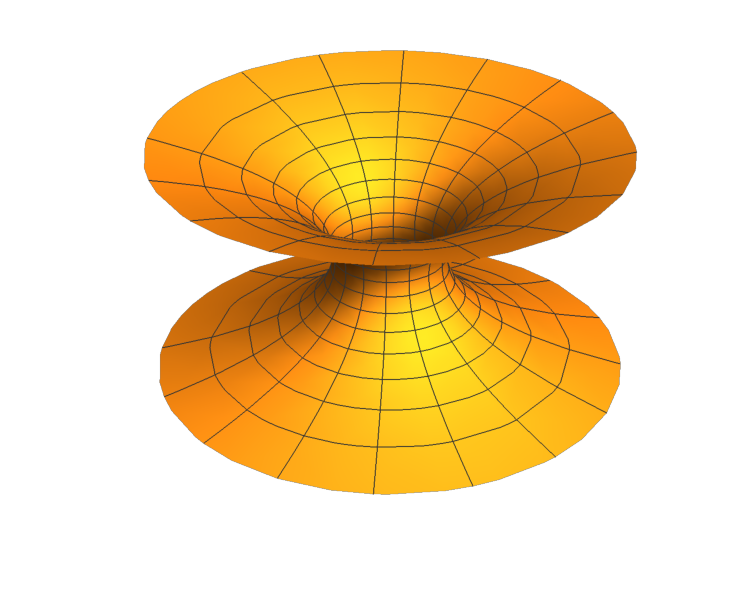
\includegraphics[scale=0.8]{images/catenoid.pdf}
\caption{Katenoida z implicitno enačbo~\eqref{eq:katenoida-implicitno}.}
\end{center}
\end{figure}

Opazimo, da je parametrizacija katenoide~\eqref{eq:katenoida} $2 \pi$-periodična glede na spremenljivko $u$. V Enneper-Weierstrassovo formulo helikatenoide~\eqref{eq:EP-helikatenoida} uvedimo novo spremenljivko $w = e^{i \zeta} \in \mathbb{C} \setminus \{0\}$ in vzemimo njen realni del. Računajmo
\begin{align*}
z(\zeta) &= (1,0,0) + \int_{0}^{\zeta} \left( \frac{1}{2} \left(\frac{1}{e^{i\xi}} - e^{i\xi} \right), \frac{i}{2} \left(\frac{1}{e^{i\xi}} + e^{i\xi} \right), 1 \right) (-i) d\xi \\
	&= (1,0,0) + \int_{1}^{w} \left( \frac{1}{2} \left(\frac{1}{\eta} - \eta \right), \frac{i}{2} \left(\frac{1}{\eta} + \eta \right), 1 \right) (-i) \frac{-i}{\eta} d\eta \\
	&= (1,0,0) - \int_{1}^{w} \left( \frac{1}{2} \left(\frac{1}{\eta} - \eta \right), \frac{i}{2} \left(\frac{1}{\eta} + \eta \right), 1 \right) \frac{d\eta}{\eta},
\end{align*}
kar nam da parametrizacijo katenoide $x \colon \mathbb{C} \setminus \{0\} \to \mathbb{R}^3$ z Enneper-Weierstrassovo formulo
\begin{equation}
x(w) = (1,0,0) - \Re \int_{1}^{w} \left( \frac{1}{2} \left(\frac{1}{\eta} - \eta \right), \frac{i}{2} \left(\frac{1}{\eta} + \eta \right), 1 \right) \frac{d\eta}{\eta}.
\end{equation}
Sledi, da je kompleksna Gaussova preslikava katenoide enaka $\mathfrak{g}(w) = w$ za $w \in \mathbb{C} \setminus \{0\}$, ki jo holomorfno razširimo do identične preslikave na $\mathbb{CP}^{1}$. Identiteta je preslikava stopnje $d=1$, zato iz teorije o Gaussovih preslikavah dobimo vrednost totalne Gaussove ukrivljenosti katenoide, ki znaša $-4 \pi$. Izkaže se, da je to edini primer iz družine pridruženih minimalnih ploskev k helikatenoidi s končno totalno Gaussovo ukrivljenostjo.

Katenoido je kot rotacijsko ploskev prvi opisal Leonhard Euler l.~1744. Dobro stoletje kasneje je P.~O.~Bonnet pokazal, da je to (razen ravnine) edina rotacijska minimalna ploskev v trirazsežnem prostoru. Ker je razmeroma enostavna in ima še več posebnih topoloških lastnosti, jo običajno spoznamo kot prvi primer pri študiju minimalnih ploskev.

%%%%%%%%%%%%%%%
% Helikoid
\subsubsection{Helikoid}
%
Negativno predznačeni imaginarni del helikatenoide imenujemo \emph{helikoid}. Natančneje, to je preslikava $y = -\Im z = \Re (iz) \colon \mathbb{R}^2 \to \mathbb{R}^3$ s konformno parametrizacijo
\begin{equation} \label{eq:helikoid}
y(u,v) = (\sin u \cdot \sinh v, -\cos u \cdot \sinh v, u).
\end{equation}
Helikoid je pridružena minimalna ploskev k helikatenoidu, ki ustreza parametrom $t = \frac{\pi}{2} + k \pi, \ k \in \mathbb{Z}$. (Res, $e^{it}z = iz$ natanko tedaj, ko je $t = \frac{\pi}{2} + 2k \pi, \ k \in \mathbb{Z}$. Z izbiro $t = \frac{\pi}{2} + k \pi, \ k \in \mathbb{Z}$, pa dobimo levi in desni helikoid.) Po definiciji sta katenoida in helikoid konjugirani minimalni ploskvi.

Geometrijsko helikoid dobimo na naslednji način: premico rotiramo okrog izbrane osi v $\mathbb{R}^3$ (tj.~v ravnini v $\mathbb{R}^3$) in jo hkrati premikamo vzdolž te osi (v pravokotni smeri glede na ravnino, v kateri premico rotiramo).

% slika helikoida
\begin{figure}[h!]
\begin{center}
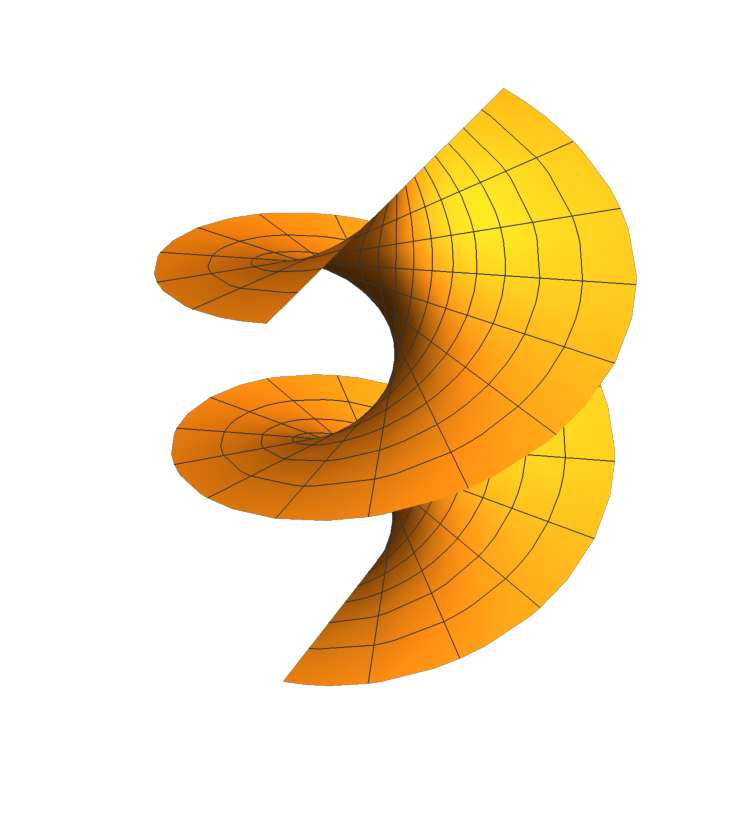
\includegraphics[scale=0.8]{images/helicoid.pdf}
\caption{Helikoid z navpično osjo kot osjo rotacije.}
\end{center}
\end{figure}

Enneper-Weierstrassovo formulo helikoida dobimo iz izraza~\eqref{eq:EP-helikatenoida}:
\begin{align}
y(\zeta) &= \Re (iz(\zeta)) = \Re \left( (i,0,0) + \int_{0}^{\zeta} \left( \frac{1}{2} \left(\frac{1}{e^{i\xi}} - e^{i\xi} \right), \frac{i}{2} \left(\frac{1}{e^{i\xi}} + e^{i\xi} \right), 1 \right) (-i) i d\xi \right) \nonumber \\
	&= \Re \int_{0}^{\zeta} \left( \frac{1}{2} \left(\frac{1}{e^{i\xi}} - e^{i\xi} \right), \frac{i}{2} \left(\frac{1}{e^{i\xi}} + e^{i\xi} \right), 1 \right) d\xi, \quad \zeta \in \mathbb{C}.
\end{align}
Njegova kompleksna Gaussova preslikava je $\mathfrak{g}(\zeta) = e^{i\zeta}$, kar nam pove, da ima helikoid negativno neskončno totalno Gaussovo ukrivljenost; $TC(y) = -\infty$. 

O helikoidu sta prva pisala L.~Euler in J.~B.~Meusnier v 80.-ih letih 18.~stoletja, brez znanja o konjugiranih minimalnih ploskvah in povezavi s kompleksno analizo. Omenimo še dve zanimivi lastnosti obravnavane minimalne ploskve:
\begin{itemize}
\item Za vsako točko na helikoidu obstaja premica, ki leži na njem, in gre skozi to točko.
\item Za vsako točko na helikoidu obstaja vijačnica, ki leži na njem, in gre skozi to točko.
\end{itemize}
Prvo lastnost kot minimalni ploskvi v $\mathbb{R}^3$ premoreta le helikoid in ravnina, kar je l.~1842 dokazal E.~C.~Catalan. Druga lastnost namiguje na izvor imena -- helikoid spominja na latinsko besedo ``helix'', kar v slovenščini imenujemo vijačnica.

%%%%%%%%%%%%%%%
% Scherkovi minimalni ploskvi
\subsubsection{Scherkovi minimalni ploskvi}
% 
Po drugi polovici 18.~stoletja je bil H.~Scherk prvi, ki je leta 1835 odkril dva nova primera -- prvo in drugo Scherkovo minimalno ploskev. 
\emph{Prvo Scherkovo ploskev} opisuje implicitna enačba
\begin{gather}
e^{z} \cos y = \cos x, \quad (x,y,z) \in \R^3.
\end{gather}
Iz enačbe vidimo, da je ploskev invariantna za translacije $(x,y,z) \mapsto (x+2\pi,y,z)$ ter $(x,y,z) \mapsto (x,y+2\pi,z)$.
Če opazujemo graf funkcije $z = \log \left(\frac{\cos x}{\cos y} \right)$ nad domeno $(x,y) \in \left( -\frac{\pi}{2}, \frac{\pi}{2} \right)^2$, opazimo asimptote:
\begin{itemize}
\item ko gre $(x,y) \to \left( \pm \frac{\pi}{2}, y \right)$ za $|y| < \frac{\pi}{2}$, gre $z \to +\infty$;
\item ko gre $(x,y) \to \left( x, \pm \frac{\pi}{2} \right)$ za $|x| < \frac{\pi}{2}$, gre $z \to -\infty$.
\end{itemize}
Prva Scherkova ploskev je kompletna. 
Njej konjugirana minimalna ploskev se imenuje \emph{druga Scherkova ploskev} z implicitno enačbo
\begin{gather}
\sin z = \sinh x \sinh y.
\end{gather}

% slika 1. in 2. Scherkove ploskve
\begin{figure}[h!]
\begin{center}
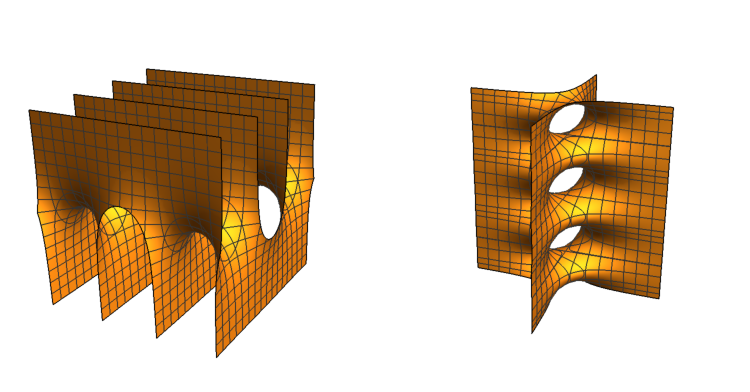
\includegraphics[scale=1.18]{images/scherk.pdf}
\caption{Prva (levo) in druga (desno) Scherkova ploskev.}
\end{center}
\end{figure}

%%%%%%%%%%%%%%%
% Enneperjeva ploskev
\subsubsection{Enneperjeva ploskev}
%
Recimo, da poznamo par $(\mathfrak{g}, \phi_3)$, kjer sta $\mathfrak{g}(z) = z$ holomorfna preslikava in $\phi_3(z) = 2z$ holomorfna 1-forma ($z \in \mathbb{C}$).
Potem po zvezi~\eqref{eq:Weierstrass-podatki-Gauss3} vemo, da je meromorfna 1-forma $\Phi$ enaka
\begin{gather*}
\Phi = \left( \frac{1}{2} \left( \frac{1}{z} - z \right), \frac{i}{2} \left( \frac{1}{z} + z \right), 1 \right) \cdot 2z = \left( 1-z^2, i(1+z^2), 2z \right).
\end{gather*}
Enneper-Weierstrassova formula preslikave $x \colon \mathbb{C} \to \mathbb{R}^3$ se glasi
\begin{equation}
x(\zeta) = \Re \int_{0}^{\zeta} \left( 1-z^2, i(1+z^2), 2z \right) dz
\end{equation}
in določa minimalno ploskev, imenovano \emph{Enneperjeva ploskev}, ki jo je l.~1868 odkril A.~Enneper.

Če za $ u,v \in \mathbb{R}$ pišemo $\zeta = u + iv \in \mathbb{C}$ in po komponentah izračunamo realne dele zgornjega integrala, dobimo konformno parametrizacijo $x \colon \mathbb{R}^2 \to \mathbb{R}^3$,
\begin{equation}
x(u,v) = \left( \frac{u}{3} \left(3(1+v^2) - u^2 \right), \frac{v}{3} \left( v^2 - 3(1+u^2) \right), u^2 - v^2 \right).
\end{equation}

% slika Enneperjeve ploskve
\begin{figure}[h!]
\begin{center}
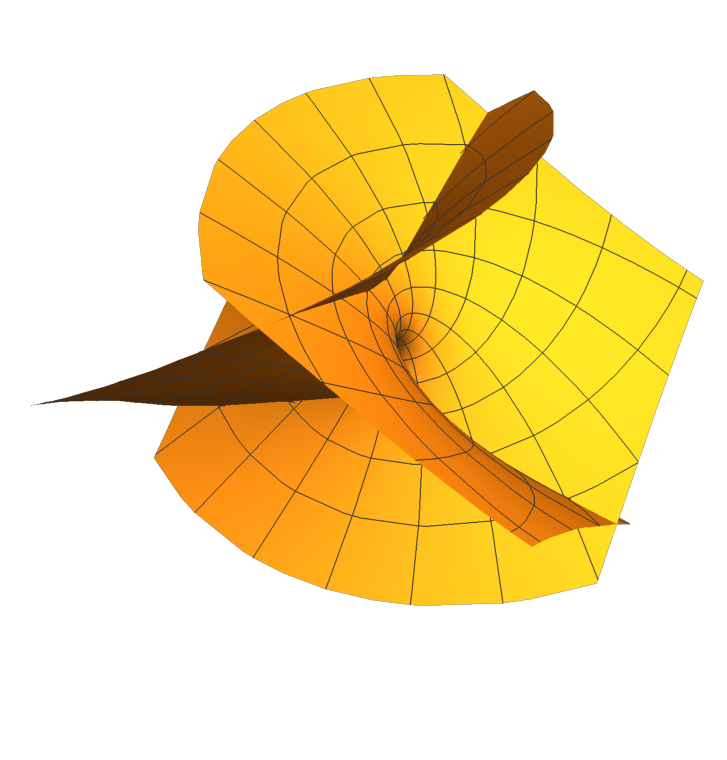
\includegraphics[scale=0.8]{images/enneper.pdf}
\caption{Enneperjeva minimalna ploskev.}
\end{center}
\end{figure}

Iz izbire podatkov vemo, da je kompleksna Gaussova preslikava Enneperjeve ploskve enaka $\mathfrak{g}(z) = z$, zato ima le-ta podobno kot katenoida totalno Gaussovo ukrivljenost enako $-4 \pi$. Izkaže se, da sta to edini kompletni neravni orientabilni minimalni ploskvi vloženi v $\mathbb{R}^3$, katerih totalna Gaussova ukrivljenost znaša $-4 \pi$. Poleg tega je Enneperjeva ploskev konjugirana sama sebi.

%%%%%%%%%%%%%%%
% Neorientabilna primera
\subsubsection{Neorientabilna primera}
%
E.~L.~Henneberg je leta 1875 odkril prvo neorientabilno minimalno ploskev v $\R^3$, ki jo imenujemo \emph{Hennebergova ploskev}.
Opisuje jo parametrizacija
%
\begin{equation}
\begin{cases}
x(u,v) = 2 \sinh u \cos v -\frac{2}{3} \sinh 3u \cos 3v \\
y(u,v) = 2 \sinh u \sin v + \frac{2}{3} \sinh 3u \sin 3v \\
z(u,v) = 2 \cosh 2u \cos 2v
\end{cases}
\end{equation}
in je bila več kot stoletje edini znan neorientabilen primer. Njena totalna Gaussova ukrivljenost je enaka $-2 \pi$, je kompletna in ima dve singularni točki.

% slika Hennebergove ploskve
\begin{figure}[h!]
\begin{center}
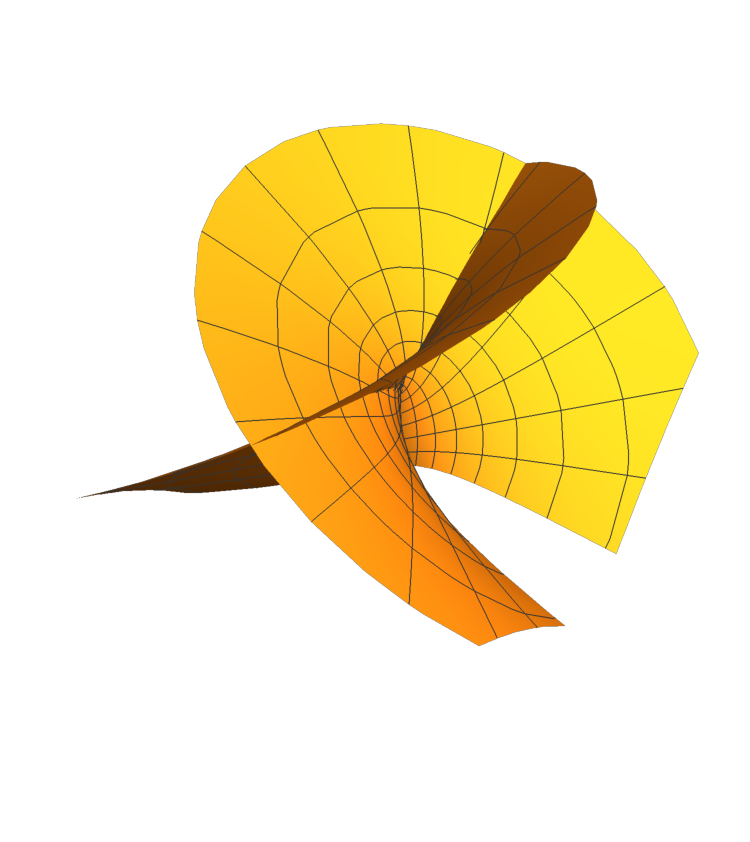
\includegraphics[scale=0.8]{images/henneberg.pdf}
\caption{Hennebergova ploskev je prva odkrita neorientabilna minimalna ploskev.}
\end{center}
\end{figure}

Znano je (\cite[Section~2.4]{alarcon2021minimal}), da je vsaka neorientabilna minimalna ploskev $S$, ki nastane z imerzijo v prostor $\R^{n}$ ($n \geq 3$), slika 2-listne konformne minimalne imerzije $x \colon M \to S \subset \R^{n}$, kjer je $M$ Riemannova ploskev.
Harmonična preslikava $x \colon \C^{*} \to \R^{3}$ s predpisom
\begin{equation*}
x(\zeta) = \Re \int_{1}^{\zeta} \left( \frac{z-1}{z^2(z+1)} - \frac{z^2(z+1)}{z-1}, i \left( \frac{z^2(z+1)}{z-1} + \frac{z-1}{z^2(z+1)} \right), 2 \right) \frac{i(z^2-1)}{2z^2} dz
\end{equation*}
definira orientabilen 2-listni krov neorientabilne minimalne ploskve, imenovane \emph{Meeksov minimalni M\"obiusov trak}. Odkril ga je W.~H.~Meeks leta 1981 in velja za prvi primer neorientabilne minimalne ploskve, ki je prava imerzija v $\R^{3}$. \newline
Kompleksna Gaussova preslikava imerzije $x$ je enaka
\begin{gather*}
\mathfrak{g}(z) = \frac{z^2(z+1)}{z-1}, \quad z \in \mathbb{CP}^1,
\end{gather*}
ki je stopnje $3$. Totalna Gaussova ukrivljenost preslikave $x$ zato znaša $-12 \pi$ in je dvakratnik totalne Gaussove ukrivljenosti Meeksovega minimalnega M\"obiusovega traku, ki je torej enaka $-6 \pi$.
Med kompletnimi neorientabilnimi minimalnimi ploskvami, ki so slike imerzij v $\R^3$, je to edina ploskev z absolutno vrednostjo totalne Gaussove ukrivljenosti, manjšo od $8 \pi$.

\clearpage
%%%%%%%%%%%%%%%%%%%%%%%%%%%%%%%%%%%%%%%%%%%%%%%%%%%%%%%%%%%%%%%%%%%%%%%%%%%%%
%%%%%%%%%%%%%%%%%%%%%%%%%%%%%%%%%%%%%%%%%%%%%%%%%%%%%%%%%%%%%%%%%%%%%%%%%%%%%
% Izreki o aproksimaciji in interpolaciji minimalnih ploskev
\section{Izreki o aproksimaciji in interpolaciji minimalnih ploskev}

Glavni cilj magistrske naloge so izreki o aproksimaciji in interpolaciji minimalnih ploskev, ki jih bomo predstavili v tem poglavju. Osnovna ideja so klasični aproksimacijski in interpolacijski izreki za holomorfne funkcije -- Rungejev, Bishop-Mergelyanov, Weierstrass-Florackov in Mittag-Lefflerjev izrek (Izreki~\ref{izr:Runge}, \ref{izr:Bishop-Mergelyan}, \ref{izr:Weierstrass-Florack}), katere je potrebno ustrezno prilagoditi.

Osredotočili se bomo na povezane odprte Riemannove ploskve $M$ z izbrano fiksno strukturo kompleksne mnogoterosti, na katerih bomo definirali konformne minimalne imerzije $x \colon M \to \mathbb{R}^{n}$ oziroma holomorfne ničelne krivulje $z \colon M \to \mathbb{C}^{n}$ ($n \geq 3$).
Zavedati se moramo, da ne moremo pričakovati izrekov v splošni obliki, kot veljajo za holomorfne funkcije. Razlog je ta, da je potrebno nadzirati periode preslikave, natančneje, ko aproksimiramo diferencial konformne minimalne imerzije, se periode diferenciala spremenijo. Aproksimacija periodno dominantnega spreja nam omogoča najti bližnjo preslikavo v novem spreju, ki ima na bazi homologije ničelne realne periode, zato po Enneper-Weierstrassovi formuli določa minimalno imerzijo.
Druga pomembna stvar pa so dopustne množice. Množice, na katerih aproksimiramo, morajo imeti končno homološko grupo. Ker vsaka odprta Riemannova ploskev premore Morsejevo funkcijo izčrpanja, ob prečkanju njene kritične točke indeksa $1$ spremembo topologije opišemo z dodajanjem vloženega loka skozi to točko. Na ta način naravno konstruiramo dopustno množico.

Poglavje sledi novejšim rezultatom, ki so predstavljeni v 3.~poglavju monografije~\cite{alarcon2021minimal}.

%%%%%%%%%%%%%%%%%%%%%%%%%%%%%%%%%%%%%%%%%%%%%%%%%%%%%%%%%%%%%%%%%%%%%%%%%%%%%
% Prostori preslikav in posplošene minimalne imerzije
\subsection{Prostori preslikav in posplošene minimalne imerzije}
%
Najprej definirajmo različne tipe konformnih minimalnih imerzij glede na njihovo sliko ter pripadajoče prostore preslikav.

% ravna, polna, neizrojena k.m.i.
\begin{definicija} \label{def:full-flat-nd}
Naj bo $M$ povezana odprta Riemannova ploskev ali kompaktna Riemannova ploskev z robom, na kateri je definirana povsod neničelna holomorfna 1-forma $\theta$. Konformno minimalno imerzijo $x \colon M \to \R^{n}$ imenujemo:
\begin{enumerate}
\item \emph{ravna}, če je slika $x(M)$ vsebovana v afini ravnini v $\R^{n}$; sicer pravimo, da je $x$ \emph{neravna};
\item \emph{polna}, če je preslikava $f = 2 \partial{x} / \theta \colon M \to \textbf{\textup{A}}_{*}^{n-1}$ polna, tj.~$\C$-linearna ogrinjača slike $f(M)$ je enaka $\C^{n}$;
\item \emph{neizrojena}, če slika $x(M)$ ni vsebovana v nobeni afini hiperravnini v $\R^{n}$. 
\end{enumerate}
\end{definicija}

V dimenziji  $n=3$ za konformno minimalno imerzijo vsi zgornji pojmi sovpadajo (\cite[Lemma~12.4]{osserman2002survey}). V višjih dimenzijah ($n \geq 4$) veljata implikaciji
\begin{gather} \label{implikacije:full-nd-nf}
\text{polna} \ \Rightarrow \ \text{neizrojena} \ \Rightarrow \ \text{neravna}.
\end{gather}
Obratne implikacije ne veljajo.

% prostori preslikav
Naj bosta $M$ in $X$ kompleksni mnogoterosti. Prostor holomorfnih preslikav $M \to X$ označimo z $\mathcal{O}(M,X)$.
Če je $K$ kompaktna podmnožica v $M$, množico preslikav $K \to X$ razreda $\mathcal{C}^{r}(M)$, ki so holomorfne v notranjosti $K^\circ \subset K$, označimo z $\mathcal{A}^{r}(K,X)$.
V primeru, ko je $X = \C$, ustrezna prostora označimo z $\mathcal{O}(M)$ oziroma $\mathcal{A}^{r}(K)$.

Naj bo $M$ odprta Riemannova ploskev in $n \geq 3$. Prostor konformnih minimalnih imerzij $M \to \R^{n}$ označimo s $\textup{CMI}(M, \R^{n})$, prostor holomorfnih ničelnih krivulj $M \to \C^{n}$ pa z $\textup{NC}(M, \C^{n})$. Oba prostora sta opremljena s kompaktno-odprto topologijo.
Nadalje $\textup{CMI}_{full}(M, \R^{n})$ in $\textup{CMI}_{nf}(M, \R^{n})$ označujeta prostora polnih oziroma neravnih konformnih minimalnih imerzij na povezanih komponentah $M$. Po zvezi~\eqref{implikacije:full-nd-nf} velja inkluzija 
\begin{gather*}
\textup{CMI}_{full}(M, \R^{n}) \subset \textup{CMI}_{nf}(M, \R^{n}).
\end{gather*}
%
Podobno je 
\begin{gather*}
\textup{NC}_{full}(M, \C^{n}) \subset \textup{NC}_{nf}(M, \C^{n})
\end{gather*} 
v primeru polnih ter neravnih holomorfnih ničelnih krivulj, saj analogna definicija k Definiciji~\ref{def:full-flat-nd} velja za holomorfne ničelne krivulje. Vsi ti prostori so odprti podprostori v $\textup{CMI}(M, \R^{n})$ oziroma $\textup{NC}(M, \C^{n})$.

Če je $M$ kompaktna Riemannova ploskev z nepraznim gladkim robom $bM$ in $r \in \N$, tedaj prostor konformnih minimalnih imerzij $M \to \R^{n}$ razreda $\mathcal{C}^{r}(M)$ označimo s $\textup{CMI}^{r}(M, \R^{n})$, prostor holomorfnih ničelnih krivulj $M \to \C^{n}$ razreda $\mathcal{C}^{r}(M)$ pa z $\textup{NC}^{r}(M, \C^{n})$.
Odprte podprostore polnih in neravnih preslikav tokrat označimo podobno kot prej; zanje velja
\begin{gather*}
\textup{CMI}_{full}^{r}(M, \R^{n}) \subset \textup{CMI}_{nf}^{r}(M, \R^{n}), \quad \textup{NC}_{full}^{r}(M, \C^{n}) \subset \textup{NC}_{nf}^{r}(M, \C^{n}).
\end{gather*}

\begin{opomba}
Imerzija $x \colon M \to \mathbb{R}^{n}$ razreda $\mathcal{C}^{r}(M)$ na kompaktni Riemannovi ploskvi z nepraznim gladkim robom $bM$ je element prostora $\textup{CMI}^{r}(M, \R^{n})$ natanko tedaj, ko je pripadajoča 1-forma $\partial x = (\partial x_{1}, \dots , \partial x_{n})$ holomorfna na $M^{\circ} = M \setminus bM$ in zadošča ničelnemu pogoju $(\partial{x_1})^2 + \cdots + (\partial{x_n})^2 = 0$.
\end{opomba}

% kompaktno-odprta C^{r} topologija
Zgoraj smo omenili kompaktno-odprto topologijo, zato jo natančneje razložimo.
Naj bosta $M$ in $X$ gladki mnogoterosti, $r \in \mathbb{N}$ in preslikava $f \colon M \to X$ razreda $\mathcal{C}^{r}(M,X)$. 
Okolico preslikave $f$ v \emph{kompaktno-odprti} ali tudi \emph{šibki} $\mathcal{C}^{r}$ topologiji na prostoru $\mathcal{C}^{r}(M,X)$ tvorijo preslikave $g \in \mathcal{C}^{r}(M,X)$, ki ustrezajo naslednji zahtevi. 
Naj bosta $K \subset M$ dana kompaktna podmnožica in $\varepsilon > 0$. Izberimo taka gladka atlasa na $M$ in $X$, ki množici $K$ in $f(K)$ pokrijeta s končno mnogo lokalnimi kartami $(U_{i}, \phi_{i})$ oz.~$(V_{i}, \psi_{i})$, pri čemer naj preslikava $f$ lokalno karto $U_{i} \subset K$ preslika v lokalno karto $V_{i} \subset f(K)$. 
Računamo $\mathcal{C}^{r}$-normo razlike preslikav $f$ in $g$ ter njunih odvodov do reda $r$ v prej izbranih parih lokalnih kart. Ustrezne so tiste preslikave $g$, za katere so vse $\mathcal{C}^{r}$-norme razlik manjše od predpisanega števila $\varepsilon$.

Opomnimo, da je topologija neodvisna od izbora atlasov na mnogoterostih oziroma lokalnih kart na $K$ in $f(K)$, čeprav je postopek iskanja okolic preslikave od teh izbir odvisen.

% lema - neravna preslikava
\begin{lema} \label{lema:neravna f}
Naj bo $M$ povezana Riemannova ploskev in $\textbf{\textup{A}}_{*}$ punktirana ničelna kvadrika.
Holomorfna preslikava $f \colon M \to \textbf{\textup{A}}_{*}$ je neravna natanko tedaj, ko je linearna ogrinjača tangentnih prostorov 
$T_{f(p)} \textbf{\textup{A}} \subset T_{f(p)} \C^{n} \cong \mathbb{C}^{n}$ po vseh $p \in M$ enaka $\C^{n}$.
\end{lema}

\begin{dokaz}
Oglejmo si preslikavo 
$\Phi \colon \C^{n} \to \C$, definirano s predpisom $\Phi(z) = \sum_{j=1}^{n} z_{j}^{2}$.
Ničelno kvadriko~\eqref{ničelna-kvadrika} tedaj lahko zapišemo v obliki $\textbf{\textup{A}} = \Phi^{-1}( \{0\} )$.
Njen tangentni prostor v točki $z = (z_{1}, \dots , z_{n}) \in \C^{n}$ je enak jedru diferenciala, ki kvadriko določa, zato je
\begin{gather*}
T_{z} \textbf{\textup{A}} = \ker \left(d \Phi_{z} \right) = \ker \left(z \mapsto \sum_{j=1}^{n} z_{j} dz_{j} \right).
\end{gather*}

Naj bosta vektorja $z, w \in \C_{*}^{n}$. Potem sta njuna tangentna prostora enaka, $ T_{z} \textbf{\textup{A}} = T_{w} \textbf{\textup{A}} $, natanko takrat, ko velja $z_{j} = \lambda w_{j}$ za vse $j = 1, \dots , n$ in nek $\lambda \in \C$, kar je ekvivalentno pogoju, da sta vektorja $z$ in $w$ kolinearna.

Po definiciji je preslikava $f$ neravna, če njena slika $f(M)$ ni vsebovana v nobeni afini kompleksni premici v $\C^{n}$. Skupaj z zgornjim je slednje ekvivalentno 
$ \mathcal{L}in \{T_{f(p)} \textbf{\textup{A}} ; \ p \in M \} = \C^{n}$, kar smo želeli dokazati.
\end{dokaz}

V aproksimacijskih in interpolacijskih izrekih bomo v dokazih namesto običajnih konformnih minimalnih imerzij in ničelnih krivulj operirali s splošnejšimi preslikavami, imenovanimi posplošene minimalne imerzije ter ničelne krivulje; naravno pa se bodo zaradi topoloških lastnosti množic, na katerih bomo preslikave aproksimirali in interpolirali, pojavile tudi množice iz naslednje definicije.

% dopustna množica
\begin{definicija} [Dopustna množica] \label{def:dopustna-mnozica}
Naj bo $M$ gladka ploskev. Kompaktno podmnožico v $M$ oblike $S = K \cup E$ imenujemo \emph{dopustna množica}, kjer je $K$ končna unija paroma disjunktnih kompaktnih domen s kosoma zvezno odvedljivimi robovi v $M$ ter $E = S \setminus K^\circ$ unija končno mnogo paroma disjunktnih gladkih Jordanovih lokov in zaprtih Jordanovih krivulj, ki se dotikajo $K$ kvečjemu v svojih krajiščih in sekajo rob $K$ transverzalno.
\end{definicija}

% posplošena konformna minimalna imerzija
\begin{definicija} [Posplošena konformna minimalna imerzija]
Naj bo $S = K \cup E$ dopustna podmnožica Riemannove ploskve $M$ in $\theta$ povsod neničelna holomorfna 1-forma, definirana v okolici $S \subset M$.
Naj bosta $n \geq 3$ in $r \in \N$. \emph{Posplošena konformna minimalna imerzija} $S \to \R^{n}$ razreda $\mathcal{C}^{r}$ je par $(x, f \theta)$, kjer je $x \colon S \to \R^{n}$ preslikava razreda  $\mathcal{C}^{r}$, njena zožitev na $S^\circ = K^\circ$ je konformna minimalna imerzija in preslikava $f \in \mathcal{A}^{r-1}(S, \textbf{\textup{A}}_{*})$ zadošča naslednjima pogojema:
\begin{enumerate}
\item na množici $K$ velja $f \theta = 2 \partial x$;
\item za vsako gladko pot $\alpha$ v $M$, ki parametrizira povezano komponento množice $E = \overline{S \setminus K}$, velja $ \Re(\alpha^{*}(f \theta)) = \alpha^{*}(dx) = d(x \circ \alpha)$.
\end{enumerate}
%
Posplošena konformna minimalna imerzija $(x, f \theta)$ je \emph{neravna} oziroma \emph{polna} natanko tedaj, ko je preslikava $f \in \mathcal{A}^{r-1}(S, \textbf{\textup{A}}_{*})$ neravna oziroma polna na vsaki relativno odprti podmnožici $S$.
\end{definicija}

Prostor posplošenih konformnih minimalnih imerzij $S \to \R^{n}$ razreda $\mathcal{C}^{r}$ označimo z $\textup{GCMI}^{r}(S, \R^{n})$. Analogno kot v primeru konformnih minimalnih imerzij velja 
\begin{gather*}
\textup{GCMI}_{full}^{r}(S, \R^{n}) \subset \textup{GCMI}_{nf}^{r}(S, \R^{n}) \subset \textup{GCMI}^{r}(S, \R^{n}).
\end{gather*}

\begin{opomba}
Spomnimo se diferenciala in konjugiranega diferenciala v kompleksnem. Zanju velja $d + i d^{c} = 2 \partial$ oziroma drugače, $\Re(2 \partial x) = dx$.
Prvi pogoj iz definicije posplošene konformne minimalne imerzije pravi $f \theta = 2 \partial x$, od koder sledi $\Re(f \theta) = \Re(2 \partial x) = dx$. Zato je drugi pogoj iz zgornje definicije skladen s prvim.
\end{opomba}

Tudi za posplošene konformne minimalne imerzije velja Enneper-Weierstrassova formula.
Naj bo $S$ povezana dopustna množica in $(x, f \theta) \in \textup{GCMI}^{r}(S, \R^{n})$. Za poljubno točko $p_{0} \in S$ in poznano preslikavo $f$ lahko posplošeno konformno minimalno imerzijo $x \colon S \to \R^{n}$ konstruiramo s formulo
\begin{gather} \label{eq:EW-gcmi}
x(p) = x(p_{0}) + \Re \int_{p_0}^{p} f \theta, \quad p \in S.
\end{gather} 
Obratno, če za preslikavo $f \in \mathcal{A}^{r-1}(S, \textbf{\textup{A}}_{*})$ velja $ \Re \int_{C} f \theta = 0$ za vsako sklenjeno krivuljo $C$ v $S$, potem le-ta določa posplošeno konformno minimalno imerzijo, dano z Enneper-Weierstrassovo formulo~\eqref{eq:EW-gcmi}.

% posplošena ničelna krivulja
\begin{definicija} [Posplošena ničelna krivulja]
Naj bo $S = K \cup E$ dopustna podmnožica Riemannove ploskve $M$ in $\theta$ povsod neničelna holomorfna 1-forma, definirana v okolici $S \subset M$.
Naj bosta $n \geq 3$ in $r \in \N$. \emph{Posplošena ničelna krivulja} $S \to \C^{n}$ razreda $\mathcal{C}^{r}$ je par $(z, f \theta)$, kjer preslikavi $z \in \mathcal{A}^{r}(S, \C^{n})$ in $f \in \mathcal{A}^{r-1}(S, \textbf{\textup{A}}_{*})$ zadoščata naslednjima pogojema:
\begin{enumerate}
\item na množici $K$ velja $f \theta = dz = \partial z$;
\item za vsako gladko pot $\alpha$ v $M$, ki parametrizira povezano komponento množice $E = \overline{S \setminus K}$ velja $ \alpha^{*}(f \theta) = \alpha^{*}(dz) = d(z \circ \alpha)$.
\end{enumerate}
%
Posplošena ničelna krivulja $(z, f \theta)$ je \emph{neravna} oziroma \emph{polna} natanko tedaj, ko je preslikava $f \in \mathcal{A}^{r-1}(S, \textbf{\textup{A}}_{*})$ neravna oziroma polna na vsaki relativno odprti podmnožici $S$.
\end{definicija}

Prostori polnih, neravnih in posplošenih ničelnih krivulj ustrezajo verigi inkluzij
\begin{gather*}
\textup{GNC}_{full}^{r}(S, \C^{n}) \subset \textup{GNC}_{nf}^{r}(S, \C^{n}) \subset \textup{GNC}^{r}(S, \C^{n}).
\end{gather*}

\begin{opomba}
Iz prvega pogoja v definiciji posplošene ničelne krivulje sledi, da je zožitev $z \colon K^{\circ} \to \mathbb{C}^{n}$ holomorfna ničelna krivulja.
\end{opomba}

Za povezano dopustno množico $S$, par $(z, f \theta) \in \textup{GNC}^{r}(S, \C^{n})$, znano preslikavo $f$ in poljubno točko $p_{0} \in S$ posplošeno ničelno krivuljo $z \colon S \to \C^{n}$ konstruiramo s pomočjo Enneper-Weierstrassove formule
\begin{gather} \label{eq:EW-gnc}
z(p) = z(p_{0}) + \int_{p_0}^{p} f \theta, \quad p \in S.
\end{gather} 
Velja tudi obrat; preslikava $f \in \mathcal{A}^{r-1}(S, \textbf{\textup{A}}_{*})$, ki zadošča $\int_{C} f \theta = 0$ za vsako sklenjeno krivuljo $C$ v $S$, določa posplošeno ničelno krivuljo, dano z Enneper-Weierstrassovo formulo~\eqref{eq:EW-gnc}.

%%%%%%%%%%%%%%%%%%%%%%%%%%%%%%%%%%%%%%%%%%%%%%%%%%%%%%%%%%%%%%%%%%%%%%%%%%%%%
% Periodno dominantni spreji
\subsection{Periodno dominantni spreji}
%
V tem razdelku bomo definirali pojem periodno dominantnega spreja holomorfnih preslikav v punktirano ničelno kvadriko. Glavni rezultat je lema, ki opisuje neravne holomorfne preslikave iz dopustne množice v punktirano ničelno kvadriko -- izkaže se, da je vsaka taka preslikava jedro periodno dominantnega spreja. Lema je pomembna pri aproksimaciji konformnih minimalnih imerzij. Natančneje, namesto imerzij bomo najprej aproksimirali periodno dominantne spreje in s tem dobili nove, bližnje preslikave z želenimi topološkimi lastnostmi, nato pa zanje uporabili Enneper-Weierstrassovo formulo ter končno dobili bližnje konformne minimalne imerzije.

\begin{definicija} [Periodna preslikava]
Naj bo $M$ povezana odprta Riemannova ploskev in $\theta$ povsod neničelna holomorfna 1-forma na $M$. Naj bo $\mathcal{C} = \{C_1, \dots , C_{l} \}$ družina gladkih orientiranih vloženih lokov in zaprtih Jordanovih krivulj v $M$ ter $C = \cup_{i=1}^{l} C_{i}$.
Družini $\mathcal{C}$ in številu $n \in \N$ priredimo \emph{periodno preslikavo}
\begin{gather}
\mathcal{P} = (\mathcal{P}_1, \dots , \mathcal{P}_{l}) \colon \mathcal{C}(C, \C^{n}) \to (\C^{n})^{l}, \nonumber \\
\mathcal{P}_{i}(f) = \int_{C_{i}} f \theta, \quad i=1, \dots , l.
\end{gather}
Tu je $f \in \mathcal{C}(C, \C^{n})$ in $\mathcal{P}_{i}(f) \in \C^{n}$.
\end{definicija}

% lema - periodno dominantni sprej 
\begin{lema} \label{lema:P-D-sprej}
Naj bo $M$ odprta Riemannova ploskev in $S = K \cup E$ dopustna množica v $M$. Naj bo $\mathcal{C} = \{C_1, \dots , C_{l} \}$ taka družina gladkih orientiranih Jordanovih krivulj in lokov v $S$, da je unija $C = \cup_{i=1}^{l} C_{i}$ Rungejeva v $S$.
Naj za neko število $r \in \Z_{+}$ preslikava $f \colon S \to \textbf{\textup{A}}_{*}$ pripada razredu $\mathcal{A}^{r}$.
Nadalje predpostavimo, da vsaka krivulja $C_{i} \in \mathcal{C}$ vsebuje netrivialen lok $I_{i} \subset C_{i}$, disjunkten z $\cup_{i \neq j}C_{j}$, preslikava $f \colon I_{i} \to \textbf{\textup{A}}_{*}$ pa je neravna.

Potem obstaja odprta okolica $U \subset \C^{ln}$ točke $0$ in preslikava $\Phi_{f} \in \mathcal{A}^{r} (S \times U, \textbf{\textup{A}}_{*})$, tako da velja
$\Phi_{f}(\cdot, 0) = f$ in je preslikava
\begin{gather} \label{PD-lastnost}
	 \frac{\partial}{\partial t} \Big|_{t=0} \mathcal{P}(\Phi_{f}(\cdot, t)) \colon (\C^{n})^{l} \to (\C^{n})^{l} \ \text{izomorfizem.}
\end{gather}

Nadalje, za končno podmnožico $P \subset S$ lahko preslikavo $\Phi_{f}$ izberemo tako, da se za $t \in U$ preslikave $\Phi_{f}(\cdot, t) \colon S \to\textbf{\textup{A}}_{*}$ ujemajo z $f$ v vsaki točki $P \setminus S^\circ$, v točkah $P \cap S^\circ$ pa se z $f$ ujemajo do danega končnega reda.

Za vsako preslikavo $f_{0} \in \mathcal{A}^{r}(S, \textbf{\textup{A}}_{*})$, ki zadošča zgornjim predpostavkam, obstaja okolica $\Omega \subset \mathcal{A}^{r}(S, \textbf{\textup{A}}_{*})$ in holomorfna preslikava $f \mapsto \Phi_{f}$, $f \in \Omega$, z zgornjimi lastnostmi.
\end{lema}

\begin{definicija} [Periodno dominantni sprej]
Preslikavo $\Phi_{f}$, ki ustreza Lemi~\ref{lema:P-D-sprej}, imenujemo \emph{periodno dominantni sprej} preslikav $S \to \textbf{\textup{A}}_{*}$ za družino krivulj $\mathcal{C}$ z \emph{jedrom} $\Phi_{f}(\cdot, 0) = f$. Lastnosti~\eqref{PD-lastnost} pravimo \emph{periodno dominantna lastnost}.
\end{definicija}

%%%%% dokaz leme
\begin{dokaz}
Prvi del leme bomo dokazali tako, da bomo konstruirali periodno dominantni sprej. Potrebovali bomo Lemo~\ref{lema:neravna f}, Bishop-Mergelyanov izrek o aproksimaciji (Izrek~\ref{izr:Bishop-Mergelyan}) in pojem toka vektorskega polja.
Zaradi enostavnosti postavimo $r=0$ (za $r>0$ dokaz poteka analogno).

Po predpostavki je za vse $i \in \{ 1, \dots, l \}$ lok $I_{i} \subset C_{i} \in \mathcal{C}$ netrivialen, za katerega velja $I_{i} \cap (\cup_{i \neq j} C_{j}) = \emptyset$ in je zožitev preslikave $f|_{I_{i}}$ neravna. Po Lemi~\ref{lema:neravna f} zato obstajajo točke $p_{i,j} \in I_{i}$ in taka holomorfna vektorska polja $V_{i,j}$ na $\C^{n}$, $j \in \{1, \dots, n \}$, ki so tangentna na $\textbf{\textup{A}}$, da je $\mathcal{L}in \{ V_{i,j}(f(p_{i,j})) ; \ j = 1, \dots, n \} = \C^{n}$ za vse $i$.

Za $k = 1, \dots , l$ označimo $t_{k} = (t_{k,1}, \dots, t_{k,n}) \in \C^{n}$ in $t = (t_{1}, \dots, t_{l}) \in \C^{nl}$. Naj $\Phi_{t}^{i,j}$ označuje tok vektorskega polja $V_{i,j}$, definiran za majhne $t$. (Seveda so tokovi holomorfne preslikave.)
Okolico $U_{0} \subset \C^{nl}$ točke $0$ izberimo tako, da za vse $t \in U_{0}$ in $p \in S$ predpis
\begin{gather} \label{predpis-tokovi}
(p, t) \mapsto \Phi_{t_{1,1}}^{1,1} \circ \cdots \circ \Phi_{t_{1,n}}^{1,n} \circ \Phi_{t_{2,1}}^{2,1} \circ \cdots \circ \Phi_{t_{l,n}}^{l,n} (f(p))
\end{gather}
podaja dobro definirano preslikavo $S \times U_{0} \to \textbf{\textup{A}}_{*}$.
Sedaj za vse pare $(i,j)$ izberimo gladke preslikave $g_{i,j} \colon C \to \C$, pri čemer je nosilec od $g_{i,j}$ vsebovan v majhnem delu loka $I_{i}$ okrog točke $p_{i,j} \in I_{i}$.
Modificirana preslikava~\eqref{predpis-tokovi}, $\Phi \colon C \times U_{1} \to \textbf{\textup{A}}_{*}$,
\begin{gather} \label{predpis-Phi}
\Phi(p,t) = \Phi_{g_{1,1}(p)t_{1,1}}^{1,1} \circ \cdots \circ \Phi_{g_{1,n}(p)t_{1,n}}^{1,n} \circ \Phi_{g_{2,1}(p)t_{2,1}}^{2,1} \circ \cdots \circ \Phi_{g_{l,n}(p)t_{l,n}}^{l,n} (f(p)),
\end{gather}
kjer je $U_{1} \subset \C^{nl}$ primerno majhna okolica točke $0$, je tedaj dobro definirana, za vse $p \in C$ pa je preslikava $\Phi(p, \cdot) \colon U_{1} \to \textbf{\textup{A}}_{*}$ holomorfna. Po lastnostih toka vektorskega polja sledi še $\Phi(p,0) = f(p)$ za vse $p \in C$ in
\begin{equation} \label{dPhi/dt}
\frac{\partial \Phi(p,t)}{\partial t_{m,j}} \Big|_{t=0} = g_{m,j}(p) \cdot V_{m,j}(f(p)).
\end{equation}

Naj bo $\mathcal{P} = (\mathcal{P}_{1}, \dots, \mathcal{P}_{l})$ periodna preslikava, prirejena družini krivulj $\mathcal{C}$. Z uporabo enakosti~\eqref{dPhi/dt} dobimo za vse indekse $i, m \in \{1, \dots, l \}$ in $j \in \{1, \dots, n \}$
\begin{gather} \label{eq:dP/dt}
\frac{\partial \mathcal{P}_{i}(\Phi(\cdot, t))}{\partial t_{m,j}} \Big|_{t=0} = \frac{\partial}{\partial t_{m,j}} \Big|_{t=0} \int_{C_{i}} \Phi(\cdot, t) \cdot \theta = \int_{C_{i}} g_{m,j} \cdot (V_{m,j} \circ f) \cdot \theta \in \C^{n}.
\end{gather}
Matrika diferencialov~\eqref{PD-lastnost} iz leme je sestavljena iz blokov velikosti $n \times n$, ki pripadajo indeksom $i, m \in \{1, \dots, l \}$. Z ustrezno izbiro preslikav $g_{i,j}$, opisanih zgoraj, lahko dosežemo, da je matrika bločno diagonalna z obrnljivimi bloki na diagonali. (To pomeni, da so vektorji~\eqref{eq:dP/dt} blizu vektorjem $V_{i,j}(f(p_{i,j}))$ za $i = m$, medtem ko so za $i \neq m$ vektorji~\eqref{eq:dP/dt} ničelni.) S tem postane celotna matrika obrnljiva.

V naslednjem koraku bomo modificirali še preslikavo $\Phi$, kar nam bo dalo iskani periodno dominantni sprej.
Preslikave $g_{i,j}$ so definirane na množici $C$, ki je po predpostavki Rungejeva v $S$. Bishop-Mergelyanov izrek o aproksimaciji pove, da vsako funkcijo $g_{i,j}$ lahko enakomerno na $C$ aproksimiramo s holomorfnimi funkcijami $\tilde{g}_{i,j}$ v okolici $S$.

Definirajmo preslikavo $\Phi_{f} \colon S \times U \to \textbf{\textup{A}}_{*}$ tako, da v predpisu~\eqref{predpis-Phi} nadomestimo $g_{i,j}$ z novimi preslikavami $\tilde{g}_{i,j}$ in je $U \subset U_{1} \subset \C^{nl}$ ustrezno majhna okolica točke $0 \in \mathbb{C}^{nl}$. Po konstrukciji takšna preslikava $\Phi_{f}$ zadošča sklepom leme, zato je periodno dominantni sprej, ki smo ga iskali.

% interpolacijski del leme
Sedaj poglejmo še interpolacijski del leme. Naj bo $P \subset S$ končna podmnožica in $q \in \mathbb{N}$ izbrano fiksno število. Vzemimo holomorfno funkcijo $h \colon S \to \mathbb{C}$, ki ima ničle natanko v točkah množice $P$, le-te pa so reda $q+1$. Kot prej obstajajo točke $p_{i,j} \in I_{i} \setminus P$, holomorfna vektorska polja $V_{i,j} \in \mathbb{C}^{n}$ ter gladke preslikave $g_{i,j}$ s kompaktnimi nosilci okrog točk $p_{i,j}$. V predpisu~\eqref{predpis-Phi} najprej nadomestimo $g_{i,j}$ s preslikavami $h \cdot g_{i,j}$, da dobimo preslikavo $\Phi$, ki zadošča analogu k~\eqref{eq:dP/dt}. Nato preslikave $g_{i,j}$ aproksimiramo z $\tilde{g}_{i,j} \in \mathcal{O}(S)$ ter v predpis~\eqref{predpis-Phi} vstavimo produkte $h \cdot \tilde{g}_{i,j}$ -- nova preslikava $\Phi_{f}$ definira periodno dominantni sprej, ki dodatno zadošča interpolacijskim zahtevam.
Res, preslikava $(p,t) \mapsto \Phi_{h(p) \tilde{g}_{m,j}(p) t}^{m,j} (f(p))$ se z $f$ ujema v točkah množice $P$, v točkah $p \in P \cap S^{\circ}$ pa se ujemata do reda $q$. (To vidimo tako, da tok vektorskega polja zapišemo s Taylorjevim razvojem do 2.~reda in upoštevamo stopnje ničel funkcije $h$ v točkah $p \in P$.) Zato enako velja tudi za njihov kompozitum (\cite[Lemma~2.2]{alarcon2018interpolation}).

Za zadnji del leme opazimo naslednje: če je preslikava $f_{0} \in \mathcal{A}^{r}(S, \textbf{\textup{A}}_{*})$ dana, potem lahko za vse preslikave $f$ iz okolice $\Omega \subset \mathcal{A}^{r}(S, \textbf{\textup{A}}_{*})$ za $f_{0}$ pri konstrukciji periodno dominantnih sprejev uporabimo iste aproksimacijske preslikave $\tilde{g}_{i,j}$.
\end{dokaz}
%%%%% konec dokaza

% globalno def. PDS
\begin{opomba} \label{op:PDS-globalno}
Če v zgornjem dokazu izberemo polna holomorfna vektorska polja $V_{i,j} \in \mathbb{C}^{n}$, namesto lokalnega konstruiramo globalno definiran periodno dominantni sprej $\Phi_{f} \colon S \times \mathbb{C}^{n} \to \textbf{\textup{A}}_{*}$.
\end{opomba}

%%%%%%%%%%%%%%%%%%%%%%%%%%%%%%%%%%%%%%%%%%%%%%%%%%%%%%%%%%%%%%%%%%%%%%%%%%%%%
% Aproksimacija in interpolacija preslikav v punktirano ničelno kvadriko
\subsection{Aproksimacija in interpolacija preslikav v punktirano ničelno kvadriko}
%
Prvi rezultat o aproksimaciji in interpolaciji je Lema~\ref{lema:aproks&interp-A*}, ki opisuje preslikave iz povezane dopustne podmnožice odprte Riemannove ploskve v punktirano ničelno kvadriko $\textbf{\textup{A}}_{*} \subset \mathbb{C}^{n}$.
V dokazu leme bomo potrebovali pojem Oka mnogoterosti, katerega definicija sledi, z lastnostjo povezanih dopustnih množic, ki premorejo končno Rungejevo bazo homologije, pa bomo lahko uporabili rezultat prejšnjega razdelka o periodno dominantnih sprejih (Lema~\ref{lema:P-D-sprej}).
Za iskanje bližnjih preslikav tistih, ki nastopajo v periodno dominantnem spreju, se bomo sklicali na različice Izrekov~\ref{izr:Runge},~\ref{izr:Bishop-Mergelyan} in~\ref{izr:Weierstrass-Florack}, tokrat za preslikave v (Oka) mnogoterosti~\cite[Theorem~1.13.1,~1.13.3]{alarcon2021minimal},
ter preslikave, definirane na dopustnih množicah~\cite[Theorem~1.12.11]{alarcon2021minimal}.
Oka mnogoterost izhaja iz \emph{Oka teorije}, imenovane po japonskem matematiku Kiyoshiju Oka, ki je v sredini 20.~stoletja prispeval veliko k razvoju kompleksne analize več spremenljivk.

% Oka mnogoterost
\begin{definicija} [Oka mnogoterost]
Naj bo $X$ kompleksna mnogoterost in $n \in \mathbb{N}$. Če za poljubno kompaktno konveksno množico $K \subset \mathbb{C}^{n}$ vsako holomorfno preslikavo $f \colon U \to X$, kjer je $U$ okolica $K$, lahko aproksimiramo enakomerno na $K$ s celimi preslikavami $F \colon \mathbb{C}^{n} \to X$, potem mnogoterosti $X$ pravimo \emph{Oka mnogoterost}.
\end{definicija}

\begin{primer} [$\textbf{\textup{A}}_{*}$ je Oka mnogoterost] \label{primer-oka}
Naj bo $z = (z_{1}, \dots , z_{n}) \in \mathbb{C}^{n}$ in $n \geq 2$. Tedaj  homogen kvadratni polinom $p(z) = z_{1}^{2} + \cdots + z_{n}^{2}$ določa ničelno kvadriko $\textbf{\textup{A}} = \{z ; \ p(z)=0 \} \subset \mathbb{C}^{n}$.
Za indekse $1 \leq i \neq j \leq n$ definirajmo holomorfna vektorska polja na $ \textbf{\textup{A}}_{*} = \textbf{\textup{A}} \setminus \{ 0 \}$ s predpisi
\begin{gather*}
V_{ij} = z_{i} \frac{\partial}{\partial z_{j}} - z_{j} \frac{\partial}{\partial z_{i}}.
\end{gather*}
Očitno so vektorska polja $\mathbb{C}$-linearna in kompletna, tangentna na punktirano ničelno kvadriko $\textbf{\textup{A}}_{*}$ in $\mathcal{L}in \{ V_{ij}(x) ; \ i,j \} = T_{x}\textbf{\textup{A}}_{*}$ v vsaki točki $x \in \textbf{\textup{A}}_{*}$. Po definiciji je zato kompleksna mnogoterost $\textbf{\textup{A}}_{*}$ fleksibilna\footnote{Pravimo, da je kompleksna mnogoterost $M$ \emph{fleksibilna}, kadar na $M$ obstaja končno mnogo takih kompletnih holomorfnih vektorskih polj $V_{1}, \dots , V_{n}$, da v vsaki točki $p \in M$ velja $\mathcal{L}in \{ V_{1}(p), \dots , V_{n}(p) \} = T_{p}M$.}, 
kar pomeni, da je tudi Oka mnogoterost (\cite[Definition~1.13.7]{alarcon2021minimal}).
\end{primer}

% [Lemma 1.12.10]
Naslednja lema, ki jo navajamo brez dokaza, trdi, da ima povezana dopustna množica posebno bazo homologije (dokaz~\cite[str.~69--71]{alarcon2021minimal}). Ideja dokaza, to je konstrukcija Jordanovih krivulj, ki tvorijo homološko bazo, bo za nas pomembna v nadaljevanju. Natančneje, pri aproksimaciji in interpolaciji minimalnih ploskev bomo interpolacijskim pogojem med drugim zadostili s kontroliranjem integralov po teh krivuljah.

\begin{lema} [Rungejeva baza homologije povezane dopustne množice] \label{lema:Runge-hom-baza}
Naj bo $S$ povezana dopustna množica. Obstaja baza homologije $\mathcal{C} = \{ C_{1}, \dots , C_{l} \}$ za $S$, sestavljena iz takih zaprtih odsekoma gladkih Jordanovih krivulj v $S$, da je unija $C = \cup_{i=1}^{l} C_{i}$ povezana in Rungejeva v vsaki regularni okolici $S_{\varepsilon}$ množice $S$, vsaka krivulja $C_{i}$ pa vsebuje netrivialen lok $I_{i}$, za katerega je $I_{i} \cap (\cup_{i \neq j} C_{j}) = \emptyset$.
Prva homološka grupa povezane dopustne množice $S$ je končno generirana: $H_{1}(S, \mathbb{Z}) \cong \mathbb{Z}^{l}$.
\end{lema}

Za $\varepsilon > 0$ je \emph{regularna okolica} dopustne množice $S \subset M$ enaka
\begin{gather}
S_{\varepsilon} = \{ x \in M; \ d(x,S) < \varepsilon \}.
\end{gather}
Množica $S_{\varepsilon}$ je odprta okolica za $S$, slednja nima lukenj v $S_{\varepsilon}$, zato je $S$ Rungejeva podmnožica svoje regularne okolice.

Sedaj imamo pripravljena vsa orodja za razumevanje aproksimacije in interpolacije preslikav v punktirano ničelno kvadriko.

% lema - aproksimacija in interpolacija preslikav v A*
\begin{lema} \label{lema:aproks&interp-A*}
Naj bo $M$ povezana odprta Riemannova ploskev in $S = K \cup E$ njena Rungejeva dopustna podmnožica.
Izberimo tako družino gladkih orientiranih Jordanovih krivulj in lokov v $S$, $\mathcal{C} = \{ C_{1}, \dots , C_{l} \}$, da je unija $C = \cup_{i=1}^{l} C_{i}$ Rungejeva v $M$, vsaka krivulja $C_{i}$ pa vsebuje netrivialen lok $I_{i}$, za katerega je $I_{i} \cap (\cup_{i \neq j} C_{j}) = \emptyset$.
Naj bo $\mathcal{P}$ periodno dominantni sprej, ki pripada družini krivulj $\mathcal{C}$, $A = \{ a_{1}, \dots , a_{m} \} \subset S$ končna množica točk in $r \geq 1$.
Tedaj lahko vsako preslikavo $f \in \mathcal{A}^{r}(S, \textbf{\textup{A}}_{*})$ aproksimiramo v $\mathcal{C}^{r}(S)$ s polnimi holomorfnimi preslikavami $F \in \mathcal{O}(M,\textbf{\textup{A}}_{*})$, pri čemer velja naslednje:
\begin{enumerate}
\item $\mathcal{P}(F) = \mathcal{P}(f)$;
\item preslikavi $F$ in $f$ se ujemata v točkah množice $A$, v točkah množice $A \cap S^{\circ}$ pa se ujemata do danega končnega reda.
\end{enumerate}
\end{lema}

%%%%% dokaz leme
\begin{dokaz}
Lemo bomo dokazali v dveh korakih. Najprej bomo $f \in \mathcal{A}^{r}(S, \textbf{\textup{A}}_{*})$ aproksimirali in interpolirali s polno preslikavo $g \in \mathcal{A}^{r}(S, \textbf{\textup{A}}_{*})$, za katero je $\mathcal{P}(f) = \mathcal{P}(g)$.
V drugem delu bomo s pomočjo Leme~\ref{lema:P-D-sprej} konstruirali periodno dominantni sprej preslikav iz množice $\mathcal{A}^{r}(S, \textbf{\textup{A}}_{*})$ z jedrom $g$. Nato bomo z izrekoma Mergelyana in Rungeja o aproksimaciji in interpolaciji preslikav iz odprtih Riemannovih ploskev v $\textbf{\textup{A}}_{*}$ periodno dominantni sprej aproksimirali in interpolirali s sprejem iz $\mathcal{O}(M, \textbf{\textup{A}}_{*})$, ki nam bo dal preslikavo $F   \in \mathcal{O}(M, \textbf{\textup{A}}_{*})$, ustrezno zaključkom leme. \newline

% 1. korak
\textit{1.~korak:} Naj bo $S = K$ povezana kompaktna množica. (Za splošnejšo dopustno množico $S = K \cup E$ je korak enak, le da ga ponovimo na vsaki povezani komponenti $K$, na $E$ pa polno preslikavo dobimo z manjšo gladko deformacijo preslikave $f$.)
Predpostavimo, da $f$ ni polna. Sicer nadaljujemo z drugim korakom.
Označimo $\Sigma(f) = \mathcal{L}in (f(K)) \subset \mathbb{C}^{n}$, ki je po predpostavki pravi podprostor v $\mathbb{C}^{n}$.
Izberimo točke $x_{1}, \dots , x_{j} \in K \setminus A$ tako, da je $\Sigma(f) = \mathcal{L}in \{ f(x_{1}), \dots , f(x_{j}) \}$.
Ker je $\dim \Sigma(f) \leq n-1$, obstaja holomorfno vektorsko polje $V$ na $\mathbb{C}^{n}$, tangentno na $\textbf{\textup{A}}$, za katerega velja $V(f(x_0)) \notin \Sigma(f)$ za neko točko $x_0 \in K \setminus (A \cup \{ x_{1}, \dots , x_{j} \})$.

Naj bosta $t \mapsto \Phi_{t}(z)$ tok vektorskega polja $V$ in $s \in \mathbb{N}$. 
Izberimo holomorfno funkcijo $h \colon K \to \mathbb{C}$ z lastnostmi:
\begin{itemize}
\item $h(x_{1}) = \dots = h(x_{j}) = 0$;
\item $h$ ima ničle reda $s$ v točkah množice $A$;
\item $h(x_0) = 1$.
\end{itemize}
Za poljubno funkcijo $\eta \in \mathcal{A}^{r}(K)$, ki je blizu ničelne funkcije, definirajmo preslikavo $\Psi (\eta) \in \mathcal{A}^{r}(K, \textbf{\textup{A}}_{*})$ s predpisom
\begin{gather}
\Psi (\eta)(x) = \Phi _{\eta(x) h(x)} f(x), \quad x \in K.
\end{gather}
Obstaja taka nekonstantna funkcija $\xi \in \mathcal{A}^{r}(K)$, ki je poljubno blizu ničelne funkcije, da je
\begin{gather*}
\mathcal{P}(\Psi (\xi)) = \mathcal{P}(\Psi(0)) = \mathcal{P}(f).
\end{gather*}
Označimo $g = \Psi(\xi)$. Velja naslednje:
\begin{itemize}
\item $g(x_{i}) = \Psi(\xi)(x_{i}) = \Phi_{\xi(x_{i}) h(x_{i})} f(x_{i}) = f(x_{i})$ za $i \in \{1, \dots , j \}$, saj je $h(x_{i})=0$. Sledi 
	$\Sigma(f) \subset \Sigma(g)$.
\item Produkt $\xi h$ je nekonstanten na kompaktu $K$, zato lahko dosežemo $\xi (x_0) \neq 0$ in $h(x_0) \approx 1.$ Potem velja
	$g(x_0) = \Psi(\xi)(x_0) = \Phi_{\xi(x_0) h(x_0)} f(x_0) \approx f(x_0) + \xi(x_0) h(x_0) V(f(x_0)) \notin \Sigma(f)$ po izboru $V$ in $x_0$.
\item Ker ima $h$ ničle reda $s$ v točkah množice $A$, s podobnim razvojem kot v prejšnji točki vidimo, da je $g|_{A} = f|_{A}$, v točkah $A \cap S^{\circ}$ pa se funkciji ujemata do reda $s$.
\end{itemize}
Induktivno nadaljujemo postopek tako, da višamo razsežnost prostora $\Sigma(f)$. Ko je $\dim \Sigma(f) = n-1$, dobimo polno preslikavo $g \in \mathcal{A}^{r}(S, \textbf{\textup{A}}_{*})$, ki aproksimira in interpolira $f$, ter zadošča pogoju $\mathcal{P}(g) = \mathcal{P}(f)$. \newline

% 2. korak
\textit{2.~korak:} Novo preslikavo $g$ iz 1.~koraka preimenujmo v $f$. Ta je polna in zato neravna.
Uporabimo Lemo~\ref{lema:P-D-sprej} in Opombo~\ref{op:PDS-globalno}, da dobimo periodno dominantni sprej $\Phi_{f} \colon S \times \mathbb{C}^{N} \to \textbf{\textup{A}}_{*}$ z jedrom $f$.

Po predpostavki je $S$ Rungejeva podmnožica $M$, iz Primera~\ref{primer-oka} pa vemo, da je kvadrika $\textbf{\textup{A}}_{*}$ Oka mnogoterost.
Izreka Rungeja in Mergelyana o aproksimaciji in interpolaciji preslikav v Oka mnogoterosti zagotavljata obstoj holomorfne preslikave $\tilde{f} \colon M \to \textbf{\textup{A}}_{*}$, ki v $\mathcal{C}^{r}(S)$ aproksimira preslikavo $f$, $\tilde{f}$ se z $f$ ujema v točkah množice $A$, v točkah preseka $A \cap S^{\circ}$ pa se ujemata do danega končnega reda.

Podobno kot v dokazu Leme~\ref{lema:P-D-sprej} lahko po Mergelyanovem izreku o aproksimaciji na dopustnih množicah funkcije $g_{i,j} \in \mathcal{A}^{r}(S)$ iz predpisa~\eqref{predpis-Phi} v $\mathcal{C}^{r}(S)$ aproksimiramo s funkcijami $\tilde{g}_{i,j} \in \mathcal{O}(M)$, tako da se $g_{i,j}$ z $\tilde{g}_{i,j}$ ujemajo na $A$ in do danega končnega reda na $A \cap S^{\circ}$.

Preslikava $\Phi_{\tilde{f}} \colon M \times \mathbb{C}^{N} \to \textbf{\textup{A}}_{*}$ ($N=ln$), definirana s predpisom
\begin{gather}
\Phi_{\tilde{f}}(p,t) = \Phi_{\tilde{g}_{1,1}(p)t_{1,1}}^{1,1} \circ \cdots \circ \Phi_{\tilde{g}_{l,n}(p)t_{l,n}}^{l,n} (\tilde{f}(p)),
\end{gather}
določa periodno dominantni sprej z jedrom $\tilde{f}$, ki aproksimira $\Phi_{f}$ na $S \times U$, kjer je $U \subset \mathbb{C}^{N}$ okolica izhodišča.
Sprej $\Phi_{f}$ zadošča periodno dominantni lastnosti, zato izrek o implicitni preslikavi zagotavlja obstoj točke $t_0 \in \tilde{U} \subset U$, za katero preslikava $F = \Phi_{\tilde{f}}(\cdot, t_0) \in \mathcal{O}(M, \textbf{\textup{A}}_{*})$ po konstrukciji izpolnjuje pogoj $\mathcal{P}(F) = \mathcal{P}(f)$, je polna ter interpolira $f$ na množici $A$.
\end{dokaz}
%%%%% konec dokaza leme

%%%%%%%%%%%%%%%%%%%%%%%%%%%%%%%%%%%%%%%%%%%%%%%%%%%%%%%%%%%%%%%%%%%%%%%%%%%%%
% Glavni izrek
\subsection{Glavni izrek}

%%%%%%%%%%%%%%%
% Nekritični primer
\subsubsection{Nekritični primer}
%
\begin{trditev} \label{trd:nekritcni-primer}
Naj bo $M$ odprta Riemannova ploskev in $\theta$ povsod neničelna holomorfna 1-forma na $M$.
Predpostavimo, da je $S$ povezana dopustna množica, ki je Rungejeva v $M$, ter $A=\{a_{1}, \dots , a_{k} \} \subset S$ končna množica točk. Naj bosta $r, s \in \N$. Tedaj velja naslednje:
\begin{enumerate}
\item 
Vsako posplošeno konformno minimalno imerzijo $(x, f\theta) \in \textup{GCMI}^{r}(S,\R^{n})$ lahko v $\mathcal{C}^{r}(S)$ aproksimiramo s polnimi konformnimi minimalnimi imerzijami $X \colon M \to \R^{n}$, za katere je $\text{Flux}_{X} = \text{Flux}_{x}$. 
\item
Vsako posplošeno ničelno krivuljo $(z, f\theta) \in \textup{GNC}^{r}(S,\C^{n})$ lahko v $\mathcal{C}^{r}(S)$ aproksimiramo s polnimi holomorfnimi ničelnimi krivuljami $Z \colon M \to \C^{n}$.
\end{enumerate}
Dodatno, preslikave $X$ oz.~$Z$ lahko izberemo tako, da se s preslikavama $x$ oz.~$z$ ujemajo v točkah množice $A$ ter do danega končnega reda v točkah množice $A \cap S^{\circ}$.
\end{trditev}

%%%%% dokaz trditve
\begin{dokaz}
Dokaz trditve je sestavljen iz dveh delov. Prvi del je algoritmičen; v njem bomo konstruirali družino krivulj, katere unija je povezana Rungejeva množica in vsebuje bazo homologije za $S$, na podoben način, kot poteka dokaz Leme~\ref{lema:Runge-hom-baza}.
V drugem delu bomo s pomočjo Leme~\ref{lema:aproks&interp-A*} našli konformno minimalno imerzijo oz.~holomorfno ničelno krivuljo, ki ustrezata zaključkom trditve.

% 1. del
Pišimo $S = K \cup E$ in naj bo $K = \cup_{i=1}^{m}K_{i}$, kjer so $K_{i}$ povezane komponente $K$. Rob vsake komponente $K_{i}$ je unija končno mnogo zaprtih Jordanovih krivulj: $bK_{i} = \cup_{j=1}^{m_{i}}\Gamma_{ij}$ za $\ m_{i} \geq 1$.
Ker je $S$ povezana, je $E = \cup_{i=1}^{n}E_{i}$, in so $E_{i}$ gladke paroma disjunktne krivulje v $S$.

Naj bo $\mathcal{C}$ Rungejeva baza homologije za $S$, konstruirana po Lemi~\ref{lema:Runge-hom-baza}.
Ker je $S$ po predpostavki Rungejeva podmnožica $M$, je družina $\mathcal{C}$ tudi baza homologije za $M$.

Množici točk $A$ iz predpostavke trditve dodajmo naslednje elemente:
\begin{itemize}
\item krajišča povezanih komponent $E_{i} \subset E = \overline{S \setminus K}$;
\item v vsaki komponenti $K_{i}$ izberimo notranjo točko $q_{i} \in K_{i}^{\circ}$, imenovano \emph{vozlišče}, in jo dodajmo v $A$;
\item točke $a_{ij} \in \Gamma_{ij}$ (za vsak par $(i,j)$ izberemo po eno tako točko), pri čemer točki $a_{ij}$ in $q_{i}$ povežemo s takim gladkim vloženim lokom $A_{ij} \subset K_{i}^{\circ} \cup \{a_{ij}\}$, da se nastali loki med seboj ter z elementi homološke baze $\mathcal{C}$ sekajo kvečjemu v vozlišču $q_{i}$. (Opomnimo, da homološko bazo povezane komponente $K_{i}$ po konstrukciji sestavlja končno mnogo Jordanovih krivulj v $K_{i}^{\circ}$, ki se dotikajo le v vozlišču $q_{i}$, njihova unija pa je Rungejeva v $K_{i}$.)
\end{itemize}
Sedaj konstruirajmo družino lokov in zaprtih krivulj $\widetilde{\mathcal{C}}$ v $S$ v treh korakih.
\begin{enumerate}
\item
	Če krivulja $C \in \mathcal{C}$ ne vsebuje elementov množice $A$ razen točke $q_{1}$, potem krivuljo $C$ dodajmo v $\widetilde{\mathcal{C}}$.
	Sicer obstaja končno točk iz $A$, ki ležijo na tej krivulji. Slednjo razdelimo na tako končno unijo lokov, da so točke iz preseka $A \cap C$ skupna krajišča dveh zaporednih lokov in vse tako nastale loke dodajmo v $\widetilde{\mathcal{C}}$.
\item
	Če obstaja krivulja $E_{k} \subset E$, ki ni vsebovana v nobeni izmed krivulj iz prejšnje točke, potem naredimo naslednje:
	krajišče od $E_{k}$, ki je element $K_{i}$ za nek $i$, povežimo z vozliščem $q_{i}$ tako, da gremo najprej po $bK_{i}$ do ustrezne točke $a_{ij}$ in nato po loku $A_{ij}$ do $q_{i}$. To ponovimo za obe krajišči $E_{k}$ in novonastalo krivuljo (ki povezuje dve -- morda isti -- vozlišči) razdelimo na končno zaporedje lokov s krajišči v točkah iz $A$ (kot v prejšnjem primeru). Vse te loke dodajmo v $\widetilde{\mathcal{C}}$.
\item
	Označimo množico $A' = \{ a \in A; \ a \ \textrm{pripada vsaj eni krivulji iz} \ \widetilde{\mathcal{C}}\}$.
	Vsaka točka njenega komplementa, tj.~$a \in A \setminus A'$, pripada neki komponenti $K_{i} \subset K$. Opazujmo sedaj take točke.
	Izberimo lok $\Lambda_{a} \subset K_{i}$, ki povezuje točko $a$ z vozliščem $q_{i}$ in se ne dotika niti nobene krivulje iz $\widetilde{\mathcal{C}}$ niti loka $\Lambda_{a'}$ za $a \neq a' \in A \setminus A'$, razen v točki $q_{i}$. (Tak lok obstaja, saj je unija krivulj iz $\widetilde{\mathcal{C}}$, konstruirane do sedaj, Rungejeva v $S$.) Vse nastale loke $\Lambda_{a}, \ a \in A \setminus A'$, dodajmo v $\widetilde{\mathcal{C}}$.
\end{enumerate}
Po konstrukciji je unija elementov družine $\widetilde{\mathcal{C}}$ povezana Rungejeva množica v $S$, ki vsebuje bazo homologije za $S$, torej tudi za $M$. Hkrati vsaka krivulja iz te družine vsebuje netrivialen lok, ki ni vsebovan v nobeni drugi krivulji iz družine. \newline

% 2. del
Naj bo $\mathcal{P}$ periodna preslikava k družini $\widetilde{\mathcal{C}}$. 
Naj bo $(x, f\theta) \in \textup{GCMI}^{r}(S, \mathbb{R}^{n})$ dana posplošena konformna minimalna imerzija. Po Lemi~\ref{lema:aproks&interp-A*} lahko preslikavo $f \in \mathcal{A}^{r-1}(S, \textup{\textbf{A}}_{*})$ v $\mathcal{C}^{r-1}(S)$ aproksimiramo s polno holomorfno preslikavo $F \in \mathcal{O}(M, \textup{\textbf{A}}_{*})$, za katero je $\mathcal{P}(F) = \mathcal{P}(f)$, $F$ se z $f$ ujema na $A$ ter do danega končnega reda na $A \cap S^{\circ}$.
Izberimo točko $p_0 \in A$ in definirajmo preslikavo $X \colon M \to \mathbb{R}^{n}$ s predpisom
\begin{gather} \label{eq:X-nekrit-primer}
X(p) = x(p_0) + \Re \int_{p_0}^{p} F\theta, \quad p \in M.
\end{gather}
Zaradi lastnosti $\mathcal{P}(F) = \mathcal{P}(f)$ je preslikava $X$ dobro definirana in po konstrukciji konformna minimalna imerzija. 
Polnost imerzije $X$ sledi iz polnosti preslikave $F$.
Nadalje je $\text{Flux}_{X} = \text{Flux}_{x}$. Res, ker $\widetilde{\mathcal{C}}$ vsebuje bazo homologije za $S$, ima $F$ ničelne realne periode po krivuljah iz homološke baze. Skupaj z definicijo preslikave $X$ in enakostjo periodnih preslikav za $F$ in $f$ sledi enakost pretokov.

Dejstvo, da $X$ aproksimira $x$ v $\mathcal{C}^{r}(S)$ drži, saj za $p \in S$ integral~\eqref{eq:X-nekrit-primer} računamo po poti med $p_0 \in A \subset S$ in $p \in S$, ki v celoti leži v $S$.

V primeru posplošene ničelne krivulje postopamo analogno: Lema~\ref{lema:aproks&interp-A*} da polno holomorfno preslikavo $F$ z lastnostmi kot prej, nato pa za izbrano fiksno točko $p_0 \in A$ definiramo preslikavo $Z \colon M \to \mathbb{C}^{n}$ s predpisom
\begin{gather} \label{eq:Z-nekrit-primer}
Z(p) = z(p_0) + \int_{p_0}^{p} F\theta, \quad p \in M,
\end{gather}
ki je polna holomorfna ničelna krivulja in aproksimira $z$ v $\mathcal{C}^{r}(S)$.

Poglejmo še interpolacijski del.
Če izberemo $p \in A$, potem integrala~\eqref{eq:X-nekrit-primer} in~\eqref{eq:Z-nekrit-primer} računamo po uniji krivulj iz družine $\widetilde{\mathcal{C}}$, ki povezuje točki $p_0, p \in A$.
Enakosti $X(p) = x(p)$ ter $Z(p) = z(p)$ sledita iz predpisov preslikav ter enakosti periodnih preslikav funkcij.
Ujemanje do danega končnega reda na množici $A \cap S^{\circ}$ pa je posledica ujemanja funkcij $F$ in $f$ do danega reda na tej isti množici.
\end{dokaz}
%%%%% konec dokaza

%%%%%%%%%%%%%%%
% Konstrukcija poti s predpisanimi integrali
\subsubsection{Konstrukcija poti s predpisanimi integrali}
%
Za začetek definirajmo nekaj pojmov iz algebraične geometrije. \newline
Naj bosta $K$ polje in $n \in \mathbb{N}$. Tedaj množico $\mathbb{A}_{K}^{n} = \{ (a_{1}, \dots , a_{n}); \ a_{1}, \dots , a_{n} \in K \}$ imenujemo $n$-razsežni \emph{afini prostor} nad poljem $K$.
Kolobar polinomov v spremenljivkah $x_{1}, \dots , x_{n}$ s koeficienti iz polja $K$ označimo s $K[x_{1}, \dots , x_{n}]$, vrednost polinoma $f \in K[x_{1}, \dots , x_{n}]$ v točki $a = (a_{1}, \dots , a_{n}) \in K^{n}$ pa z $f(a)$.
Nadalje je množica $V(f_{1}, \dots , f_{m}) = \{ x \in \mathbb{A}_{K}^{n} ; \ f_{i}(x) = 0, \ f_{i} \in K[x] \ \textrm{za vse} \ i = 1, \dots , m \} \subset \mathbb{A}_{K}^{n}$ \emph{afina raznoterost}.

V primeru, ko je $z = (z_{1}, \dots , z_{n}) \in \mathbb{C}^{n}$, funkcije $f_{1}, \dots , f_{m}$ pa so holomorfni polinomi, množici
\begin{gather}
V(f_{1}, \dots , f_{m}) = \{ z \in \mathbb{C}^{n}; \ f_{1}(z) = \dots = f_{m}(z) = 0 \}
\end{gather}
pravimo \emph{afina algebraična raznoterost}, ki je hkrati zaprta kompleksna podraznoterost raznoterosti $\mathbb{C}^{n}$.
V nadaljevanju se bomo ukvarjali z le-temi.

Če afine algebraične raznoterosti $A$ ne moremo zapisati kot unijo dveh neničelnih afinih algebraičnih raznoterosti, potem $A$ imenujemo \emph{nerazcepna raznoterost}.
Sicer je $A$ \emph{razcepna}.

Pogosto nas zanimajo le regularne ali singularne točke. Zato uvedimo posebni oznaki:
množico regularnih točk raznoterosti $A$ označimo z $A_{reg}$, množico singularnih točk raznoterosti $A$ pa z $A_{sing}$.

Pravimo, da je afina algebraična raznoterost, ki je podraznoterost v $\mathbb{C}^{n}$, \emph{neizrojena}, kadar ni vsebovana v nobeni afini hiperravnini v $\mathbb{C}^{n}$.

% Lema: poti s predpisanimi integrali, analog Gromova
\begin{lema} \label{lema:analog-gromova}
Naj bo $A$ nerazcepna neizrojena algebraična podraznoterost v $\mathbb{C}^{n}$, $\eta \in \mathbb{C}^{n}$ izbran vektor in $\Omega \subset \mathbb{C}^{n}$ povezana domena, ki vsebuje $0$ in $\eta$. 
Naj bosta dani zvezni preslikavi $f_0 \colon [0,1] \to A_{reg}$ in $g \colon [0,1] \to \mathbb{C}_{*}$.
Potem za $\tau \in [0,1]$ obstaja taka homotopija $f_{\tau} \colon [0,1] \to A_{reg}$ s fiksnima krajiščema, da je $f_0$ dana preslikava, preslikava $f = f_1$ je gladka in neravna v okolici $f(0)$, ter velja
\begin{gather} \label{eq:pot-s-predp-integralom}
\int_{0}^{1} f(s)g(s)ds = \eta \quad \textrm{in} \quad \int_{0}^{t} f(s)g(s)ds \in \Omega \quad \textrm{za vse} \ t \in [0,1].
\end{gather}
Natančneje, za poljuben par točk v $A_{reg}$ obstaja gladka pot $f \colon [0,1] \to A_{reg}$ med njima, ki zadošča pogoju~\eqref{eq:pot-s-predp-integralom}.
\end{lema}

Navedli bomo le osnovne ideje dokaza leme. Popoln dokaz, ki se nahaja v~\cite[Lemma~3.5.4]{alarcon2021minimal}, posnema dokaz leme Mikhaila Gromova\footnote{Mikhail Gromov, roj.~1943, je rusko-francoski matematik s področij geometrije, analize in teorije grup. Med drugim je uvedel metodo kompleksne integracije, h-princip in pojem skoraj ravne mnogoterosti. Leta 2009 je prejel Abelovo nagrado.}
o konveksni integraciji. Rezultat je pomemben, ker nam omogoča konstrukcijo poti s predpisanimi vrednostmi integralov znotraj množice regularnih točk nerazcepne algebraične raznoterosti. Mi jo bomo uporabljali za konstrukcijo poti v punktirani ničelni kvadriki $\textup{\textbf{A}}_{*} \subset \C^{n}$ v dokazu Glavnega izreka~\ref{izr:glavni-izrek-CMI}.

% dokaz leme
\begin{dokaz}
Dokaz poteka v štirih korakih.

\textit{1.~korak:} Pokažemo, da zadostuje rešiti bližnji problem, kjer pogoja~\eqref{eq:pot-s-predp-integralom} nadomestimo s pogojema
\begin{gather} \label{eq:pot-s-predp-integralom-bliznja}
\left| \int_{0}^{1} f(s)g(s)ds - \eta \right| < \varepsilon \quad \textrm{in} \quad \int_{0}^{t} f(s)g(s)ds \in \Omega \quad \textrm{za vse} \ t \in [0,1]
\end{gather}
za $\varepsilon > 0$.
Pišemo $[0,1] = [0,c] \cup [c,1]$ za $c \in (0,1)$.
Podobno kot v dokazu Leme~\ref{lema:P-D-sprej} poiščemo periodno dominantni sprej preslikave $f_0$ z nosilcem na intervalu $(0,c)$.
Sledi, da je dovolj najti homotopijo $f_{\tau} \colon [0,1] \to A_{reg}$, ki je fiksna na $[0,c]$, pot $f = f_{1}$ pa zadošča pogojema~\eqref{eq:pot-s-predp-integralom-bliznja}. Napake $\varepsilon$ se znebimo tako, da $f$ nadomestimo s potjo $\Phi_{f}(\zeta, \cdot) \colon [0,1] \to A_{reg}$, kjer je sprej $\Phi_{f}$ definiran analogno spreju, prirejenemu $f_0$, in izberemo ustrezen parameter $\zeta \in \mathbb{B}^{n} \subset \mathbb{C}^{n}$. \newline

\textit{2.~korak:} Problem poenostavimo na problem, kjer $\Omega$ vsebuje $\{ s\eta; \ s \in [0,1] \}$. \newline
Izberemo poligonsko pot $\Gamma = \cup_{j=1}^{m} \Gamma_{j} \subset \Omega$ med $0$ in $\eta$, kjer za $p_{j-1} \in \Omega$ in $\eta_{j} \in \mathbb{C}^{n}$ pišemo $\Gamma_{j} = \{ p_{j-1} + s\eta_{j}; \ s \in [0,1] \}$.
Velja $\eta = \sum_{j=1}^{m} \eta_{j}$.
Tedaj iščemo deformacijo $f(s)$ za $f_0(s)$, ki je fiksna v okolici točk $s = 0, 1, \dots , m$ in zanjo velja
\begin{gather*}
\left| \int_{j-1}^{j} f(s)g(s)ds - \eta_{j} \right| < \frac{\varepsilon}{m} \quad \textrm{in} \quad \int_{j-1}^{t} f(s)g(s)ds \in \Omega_{j} \quad \textrm{za vse} \ t \in [j-1,j],
\end{gather*}
kjer je $\Omega_{j}$ okolica za $\{ s \eta_{j}; \ s \in [0,1] \}$. \newline

\textit{3.~korak:} Ohranimo redukcijo iz 2.~koraka in rešimo problem za $0 \neq g = konst.$ \newline

\textit{4.~korak:} Rešimo splošen primer. \newline
Izberemo števili $\sigma > 0$ in $N \in \mathbb{N}$, ter interval $[0,1]$ razdelimo na unijo podintervalov: $[0,1] = \cup_{j=1}^{N} I_{j} = \cup_{j=1}^{N} [\frac{j-1}{N}, \frac{j}{N}]$. Pri tem zahtevamo, da na vsakem podintervalu $I_{j}$ obstaja taka neničelna konstantna funkcija $g_{j}$, da na njem velja $|g - g_{j}| < \sigma$.
Postopek iz 3.~koraka ponovimo na vsakem podintervalu $I_{j}$ -- zadostiti moramo pogojema~\eqref{eq:pot-s-predp-integralom-bliznja}, pri čemer $g$ nadomestimo z $g_{j}$ na ustreznih intervalih $I_{j}$.
Velja
\begin{gather*}
\left| \int_{I_{j}} f(s)g(s)ds - \int_{I_{j}} f(s)g_{j}(s)ds \right| \leq \frac{R}{N} \cdot \max_{I_{j}} |g - g_{j}| < \frac{R}{N} \sigma,
\end{gather*}
saj je $|I_{j}| = 1/N$ za vse $j$ in $|f| \leq R$ za nek $R > 0$.
Vsota napak po vseh podintervalih je torej navzgor omejena z $R \sigma$. Ta bo poljubno majhna za izbor poljubno majhnega $\sigma >0$.
Ker znamo rešiti bližnji problem~\eqref{eq:pot-s-predp-integralom-bliznja} v splošnem primeru, po 1.~koraku lema sledi.
\end{dokaz}

%%%%%%%%%%%%%%%
% Morsejeva teorija in ročajniki
\subsubsection{Morsejeva teorija in ročajniki}
%
V tem razdelku bomo navedli nekaj osnovnih rezultatov Morsejeve teorije. Pokazali bomo, kako gladke mnogoterosti (v našem -- posebnem -- primeru ploskve) predstavimo kot ročajnike. Znanje tega razdelka nam bo koristilo pri dokazovanju glavnega izreka o aproksimaciji in interpolaciji minimalnih ploskev.
   
Naj bo $U \subset \mathbb{R}^{n}$ domena s koordinatami $x = (x_{1}, \dots , x_{n})$ in $f \colon U \to \mathbb{R}$ funkcija razreda $\mathcal{C}^{2}$.
Spomnimo se, da je točka $x \in U$ \emph{kritična točka} funkcije $f$, če je $\nabla f(x) = 0$. Točka, ki ni kritična, je \emph{regularna}.
Slike kritičnih točk imenujemo \emph{kritične vrednosti}, medtem ko so vsa preostala realna števila \emph{regularne vrednosti} funkcije $f$. \newline
%
\emph{Hessejeva forma} funkcije $f$ v točki $x \in U$ je simetrična kvadratna forma $\text{Hess}_{f}(x)$ na tangentnem prostoru $T_{x}\R^{n} = \R^{n}$, pripadajoča Hessejeva matrika $H_{f}(x)$ pa sestoji iz drugih odvodov funkcije $f$ v točki $x$. Velja $H_{f}(x) = D(\nabla f)(x)$, kjer $D$ označuje Jacobijevo matriko.

\begin{definicija}
Naj bo $x \in U$ kritična točka funkcije $f$. Kadar ima pripadajoča Hessejeva matrika $H_{f}(x)$ maksimalen rang, točki $x$ pravimo \emph{Morsejeva točka}. Slednji pogoj je ekvivalenten trditvi, da je Hessejeva forma funkcije $f$ v točki $x$ neizrojena.

Število negativnih lastnih vrednosti Hessejeve matrike, $k \in \{0,1, \dots , n\}$, je \emph{Morsejev indeks} kritične točke.

Funkcija, katere vsaka kritična točka je tudi Morsejeva, se imenuje \emph{Morsejeva funkcija}.
\end{definicija}

Kritične točke funkcije $f$ dobimo z reševanjem enačbe $\nabla f(x)=0$. Ker je Hessejeva matrika enaka Jacobijevi matriki gradienta funkcije, po izreku o inverzni preslikavi vidimo, da je vsaka kritična točka izolirana. Množica kritičnih točk funkcije $f$, $\text{Crit}(f) = \{ x \in U; \ \nabla f(x)=0 \}$, je zaprta diskretna podmnožica v $U$.

% funkcija izčrpanja
\begin{definicija}
Naj bosta $M$ mnogoterost in $f \colon M \to [0, \infty)$ zvezna funkcija. Če je za vsako realno število $c>0$ množica $M_{c} = \{ p \in M; \ f(p) \leq c \}$ kompaktna, tedaj $f$ imenujemo \emph{funkcija izčrpanja} mnogoterosti $M$.
\end{definicija}

Za nas bodo pomembne Morsejeve funkcije izčrpanja na Riemannovih ploskvah. Njihov obstoj opisuje naslednja trditev~\cite[Proposition~1.12.5]{alarcon2021minimal}.

\begin{trditev} \label{trd:Riem-ploskev-Morse-izcrpanje}
Naj bo $K$ kompaktna $\mathcal{O}(M)$-konveksna podmnožica odprte Riemannove ploskve $M$ in $U \subset M$ odprta množica, ki vsebuje $K$.
Tedaj na $M$ obstaja strogo subharmonična Morsejeva funkcija izčrpanja $\rho$, za katero velja 
\begin{gather*}
K \subset \{ \rho<0 \} \subset \{ \rho \leq 0 \} \subset U.
\end{gather*}
\end{trditev}

Po zgornji trditvi lahko mnogoterost $M$ konstruiramo s pomočjo njene funkcije izčrpanja $\rho$, natančneje, podnivojnicam $\{ \rho \leq c \}$ ob prehodu kritičnih točk funkcije izčrpanja zaporedoma dodajamo t.~i.~ročaje. V tem primeru pravimo, da mnogoterost predstavimo kot \emph{ročajnik}. Pomemben izrek Morsejeve teorije, ki ga bomo navedli v nadaljevanju, ta postopek natančno opisuje. Pred tem definirajmo ustrezne pojme, ki so povzeti po~\cite[Section~1.4]{alarcon2021minimal}.

% ročajnik
Vzemimo gladko mnogoterost $M$ z robom $bM$ razsežnosti $\dim M = m \in \mathbb{N}$.
Naj bo $k \in \{1, 2, \dots , m\}$, $m = k+q$ in naj $\mathbb{D}^{k} \subset \mathbb{R}^{k}$ označuje zaprto $k$-razsežno enotsko kroglo. Kartezičnemu produktu
\begin{gather*}
H = H^{k,q} = \mathbb{D}^{k} \times \mathbb{D}^{q}
\end{gather*}
pravimo \emph{standardni ročaj} indeksa $k$ in dimenzije $m$. Podmnožico $E = \mathbb{D}^{k} \times \{0\}^{q} \subset H$ imenujemo \emph{stržen} ročaja, podmnožico $F = b\mathbb{D}^{k} \times \mathbb{D}^{q} = \mathbb{S}^{k-1} \times \mathbb{D}^{q} \subset H$ pa njegova \emph{priključna množica}. \newline
Definirajmo preslikavo
\begin{gather*}
\phi \colon \mathbb{S}^{k-1} \times \mathbb{D}^{q} \to bM
\end{gather*}
med priključno množico in robom mnogoterosti, ki naj bo gladek difeomorfizem na sliko. Vzemimo disjunktno unijo mnogoterosti in standardnega ročaja, $M \sqcup H$, ter točke priključne množice $F$ identificirajmo s svojimi slikami. Preslikava $\phi$ je lepilna preslikava pri lepljenju ročaja indeksa $k$ na mnogoterost $M$. Tako nastalo množico 
\begin{gather*}
\widetilde{M} = M \sqcup_{\phi} H
\end{gather*}
imenujemo \emph{ročajnik}.
Z ``glajenjem'' vzdolž množice $\phi(\mathbb{S}^{k-1} \times \mathbb{S}^{q-1})$ dosežemo, da ročajnik postane gladka mnogoterost z robom. V nadaljevanju bomo predpostavili, da so ročajniki takšni.

% [Theorem 1.4.7]
\begin{izrek} \label{izr:rocajnik}
Naj bo $M$ gladka mnogoterost razsežnosti $\dim M= m$. Naj bo $\rho \colon M \to \mathbb{R}$ gladka Morsejeva funkcija, števili $a<b$ njeni regularni vrednosti in
\begin{gather*}
M_{a,b} = \{ x \in M; \ a \leq \rho(x) \leq b \}
\end{gather*}
kompaktna množica.
\begin{enumerate}
\item Recimo, da množica $M_{a,b}$ ne vsebuje nobene kritične točke Morsejeve funkcije $\rho$. Potem so za vse vrednosti $t \in [a,b]$ podnivojnice 
	$M_{t} = \{ x \in M; \ \rho(x) \leq t \}$ paroma difeomorfne.
\item Kadar množica $M_{a,b}$ vsebuje natanko eno kritično točko Morsejeve funkcije $\rho$, ta pa ima Morsejev indeks enak $k$, tedaj je podnivojnica 
	$M_{b}$ difeomorfna ročajniku, sestavljenemu iz podnivojnice $M_{a}$ in ročaja indeksa $k$.
	Če je $k=0$, je $M_{b}$ difeomorfna disjunktni uniji $M_{a}$ in kompaktne $m$-razsežne krogle $\mathbb{D}^{m}$.
\end{enumerate}
\end{izrek}

Osredotočimo se na orientabilne ploskve in s pomočjo Izreka~\ref{izr:rocajnik} obravnavajmo njihovo ročajno strukturo. 
Izberimo gladko orientabilno ploskev $M$ in pripadajočo gladko Morsejevo funkcijo izčrpanja $\rho \colon M \to [0, \infty)$. Če je $c$ regularna vrednost funkcije izčrpanja, potem je podnivojnica $M_{c} = \{ \rho \leq c \}$ kompaktna ploskev, njen rob $bM_{c} = \{ \rho = c \}$ pa končna unija gladkih Jordanovih krivulj. 

Po prvi točki Izreka~\ref{izr:rocajnik} je za taki regularni vrednosti $a<b$, da množica $M_{a,b} = \{ x \in M; \ a \leq \rho(x) \leq b \}$ ne vsebuje nobene kritične točke funkcije $\rho$, slednja množica končna unija kompaktnih kolobarjev. Število kolobarjev je enako številu povezanih komponent roba $bM_{a}$.

Pri prehodu kritičnih točk funkcije $\rho$ pa podnivojnicam dodajamo ročaje ustreznih indeksov, kar nam pove druga točka Izreka~\ref{izr:rocajnik}.

% indeks = 0
V kritični točki indeksa $0$, ki je lokalni minimum, podnivojnici disjunktno dodamo novo povezano komponento, kompakten disk.

% indeks = 1
Če je $p \in M$ kritična točka indeksa $1$, ki naj bo brez škode za splošnost edina kritična točka na nivojnici $\{ \rho = \rho(p) \}$, izberimo bližnji vrednosti $a<\rho(p)<b$ tako, da je točka $p$ edina kritična točka na množici $M_{a,b}$. Podnivojnica $M_{b}$ nastane tako, da na $M_{a}$ ustrezno prilepimo ročaj indeksa $1$, to je $H = [-1,+1] \times [-1,+1]$. Pri tem komponenti roba ročaja, $\{-1\} \times [-1,+1]$ in $\{+1\} \times [-1,+1]$, difeomorfno zlepimo z disjunktnima lokoma $I_{-1}, I_{+1} \subset bM_{a}$.
\begin{itemize}
\item[\textit{(a)}] 
	Če loka $I_{-1}, I_{+1}$ pripadata isti povezani komponenti $bM_{a}$, za rodova velja $\text{gen}(M_{a}) = \text{gen}(M_{b})$, število povezanih komponent nivojnice $bM_{b}$ pa je za ena več od števila povezanih komponent nivojnice $bM_{a}$.
\item[\textit{(b)}]
	Če loka $I_{-1}, I_{+1}$ pripadata isti povezani komponenti $M_{a}$, a različnima povezanima komponentama $bM_{a}$, je situacija naslednja.
	Množica $M_{a,b}$ je unija končno mnogo paroma disjunktnih kolobarjev in \emph{para hlač}, ki je kompaktna ploskev topološkega rodu $1$, katere rob sestoji iz treh povezanih komponent.
	Velja $\text{gen}(M_{a})+1 = \text{gen}(M_{b})$, število povezanih komponent roba $bM_{b}$ pa je za ena manj od števila povezanih komponent roba $bM_{a}$.
\item[\textit{(c)}]
	Če loka $I_{-1}, I_{+1}$ pripadata različnima povezanima komponentama podnivojnice $M_{a}$, je $\text{gen}(M_{a}) = \text{gen}(M_{b})$, rob $bM_{b}$ pa ima eno povezano komponento manj od roba $bM_{a}$.
\end{itemize}

% slika ročajnikov
\begin{figure}[h!]
\begin{center}
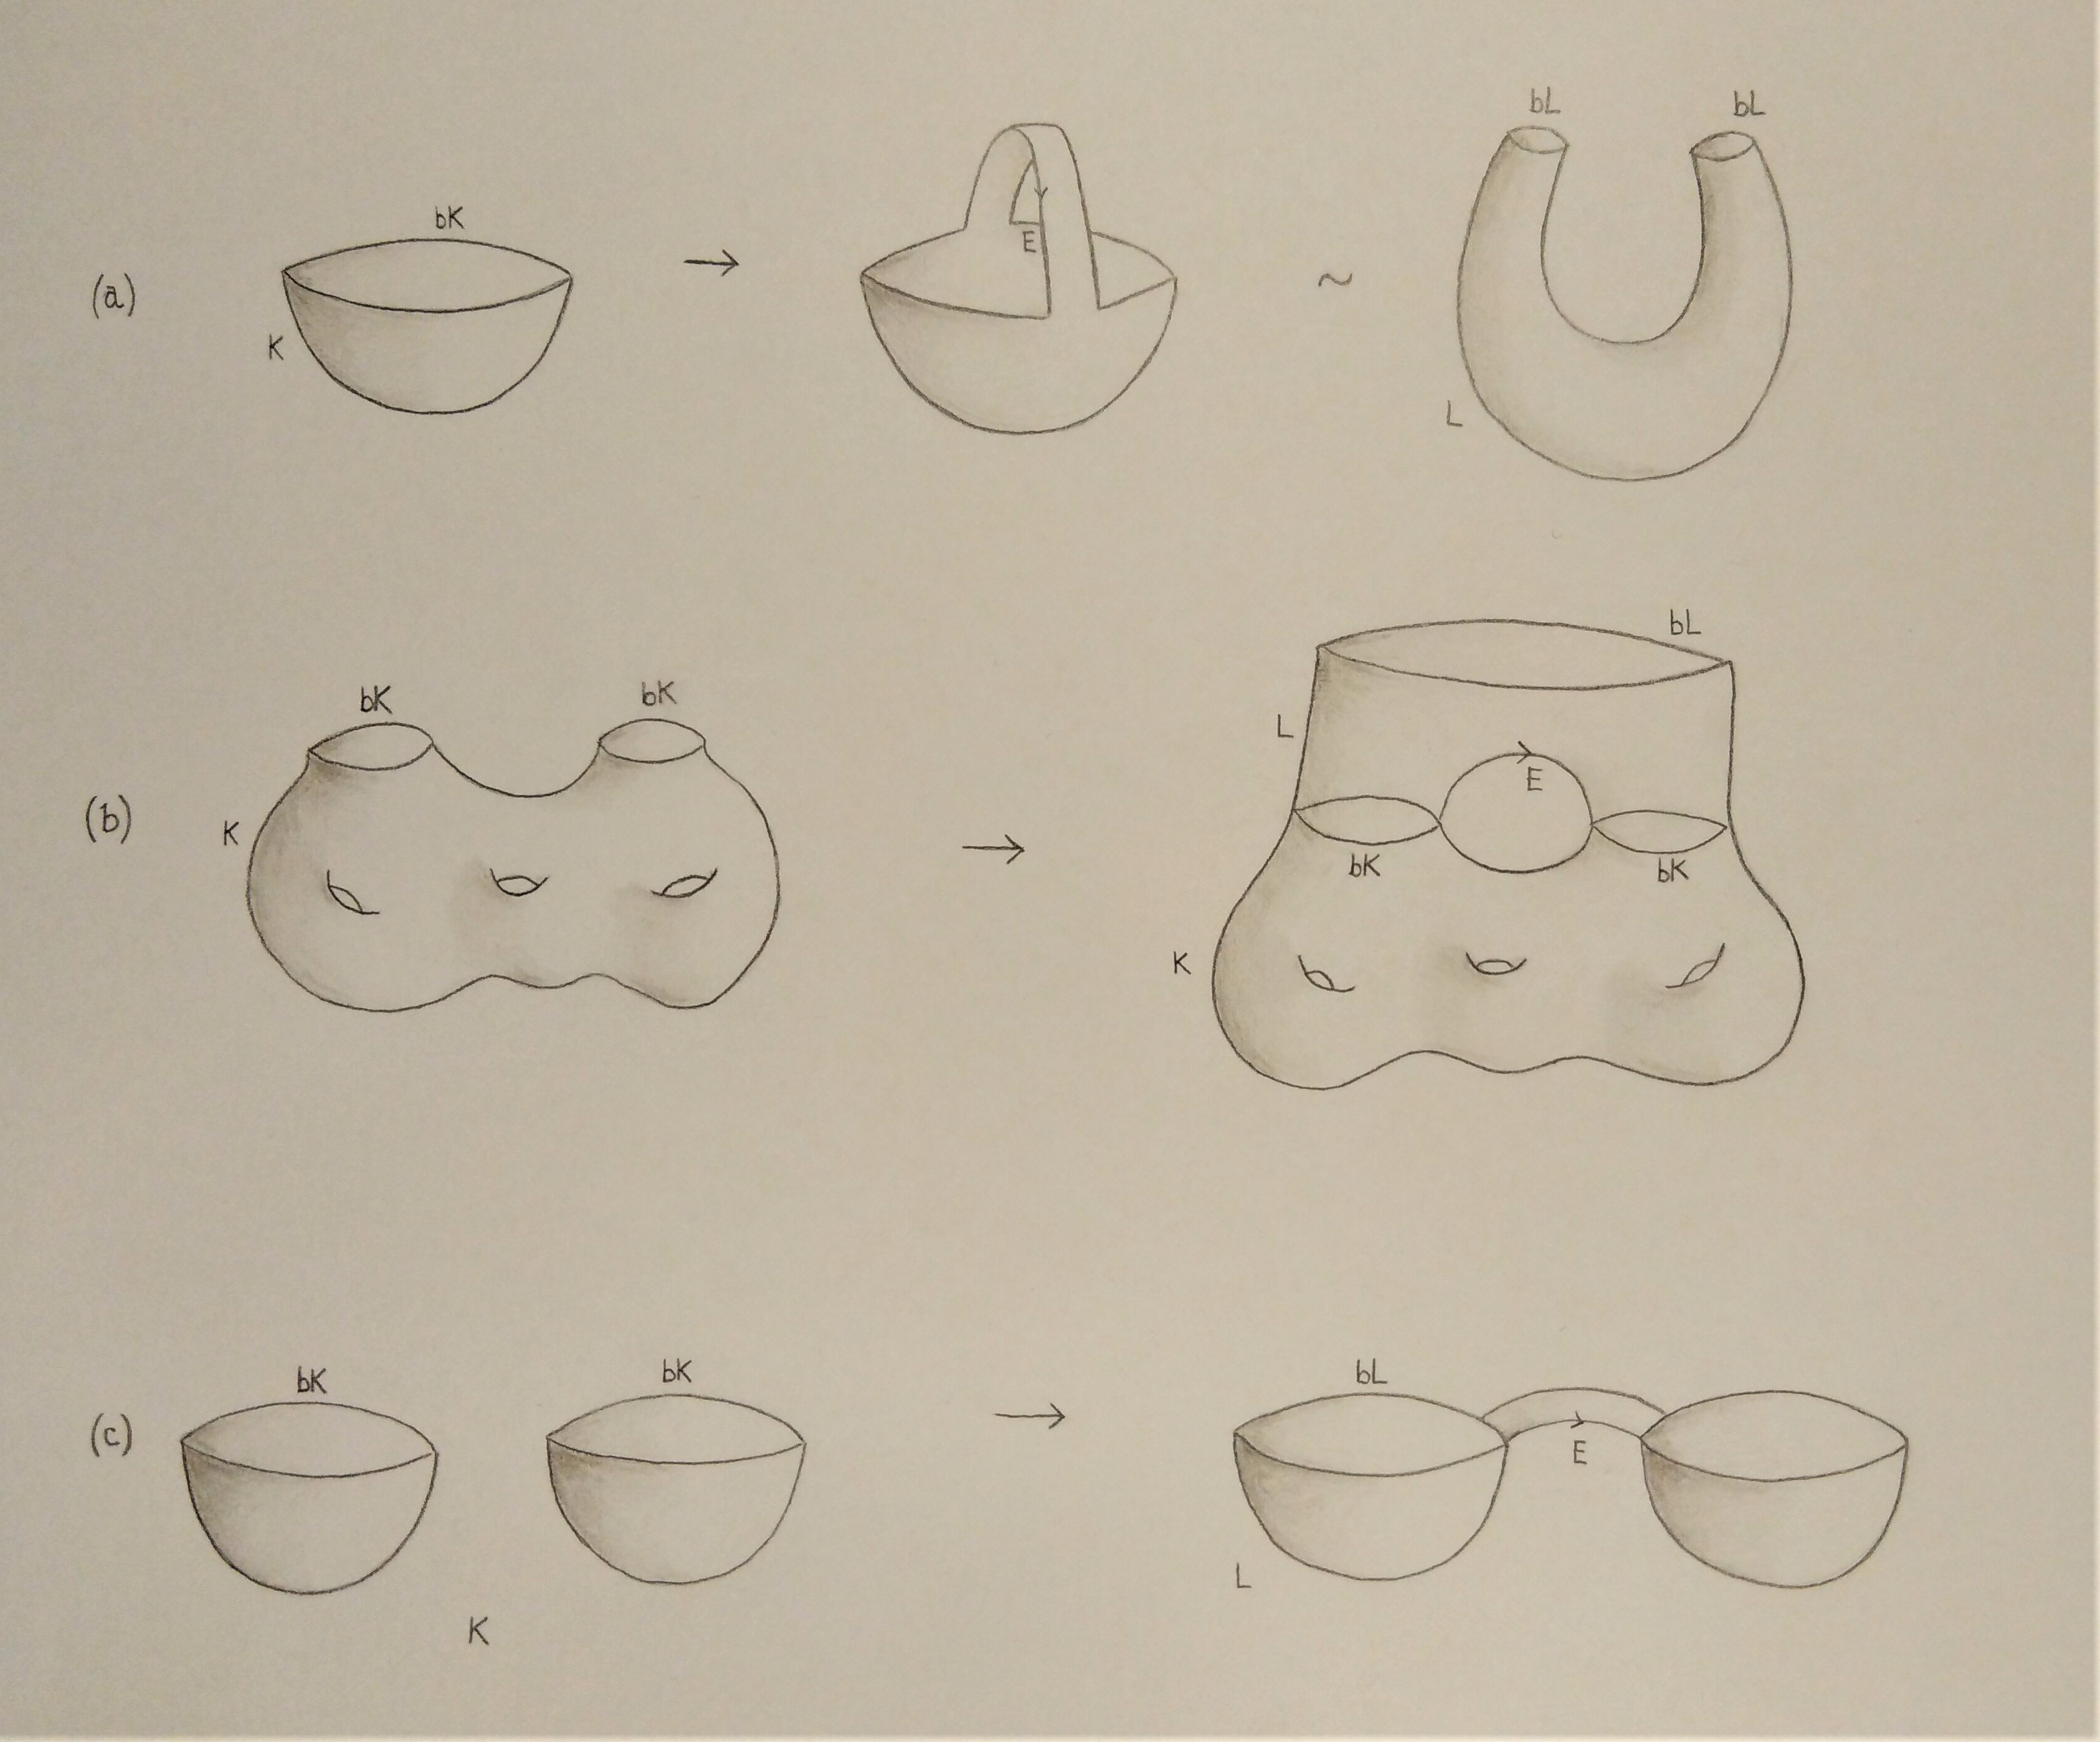
\includegraphics[scale=0.12]{images/morse.jpg}
\caption{Spremembe topologije ploskve pri prehodu kritične točke Morsejevega indeksa $1$ v primerih \textit{(a)--(c)}. Zgornji del $L \setminus K$ druge slike v primeru \textit{(b)} je par hlač.}
\end{center}
\end{figure}

% indeks = 2
V kritični točki maksimalnega indeksa (v našem primeru ploskve je ta enak $2$), ki je lokalni maksimum, na podnivojnico nalepimo disk maksimalne razsežnosti (v našem primeru $2$).

\begin{opomba} [Rod ploskve]
Znano je, da je povezana kompaktna orientabilna ploskev $M$ brez roba homeomorfna bodisi sferi $\mathbb{S}^{2}$ bodisi vsoti $g$ torusov 
$\mathbb{T}^{2} \# \stackrel{g}{\cdots} \# \mathbb{T}^{2}$ za enolično število $g \in \mathbb{N}$.
Število $g$ imenujemo \emph{rod} in označimo z $\text{gen}(M)$, pri tem pa definiramo še $\text{gen}(\mathbb{S}^{2}) = 0$.
Podobna klasifikacija velja za odprte orientabilne ploskve.
\end{opomba}

%%%%%%%%%%%%%%%
% Glavni izrek
\subsubsection{Glavni izrek}
%
Sedaj bomo navedli in dokazali glavni rezultat, to je izrek o aproksimaciji in interpolaciji konformnih minimalnih imerzij iz odprtih Riemannovih ploskev v Evklidski prostor $\mathbb{R}^{n}$ razsežnosti vsaj $3$. Izrek združuje aproksimacijo Mergelyanovega tipa z Weierstrassovo interpolacijo, kot jo v primeru holomorfnih funkcij podajata Izreka~\ref{izr:Bishop-Mergelyan} in~\ref{izr:Weierstrass-Florack}.
Analogen rezultat velja za holomorfne ničelne krivulje.

\begin{izrek} \label{izr:glavni-izrek-CMI}
Naj bo $M$ odprta Riemannova ploskev, $\theta$ povsod neničelna holomorfna 1-forma na $M$, $n \geq 3$ in $r \geq 1$.
Naj bo $S$ dopustna Rungejeva množica v $M$ in $\Lambda \subset M$ zaprta diskretna podmnožica. 
Naj bo $x \colon S \to \R^{n}$ posplošena konformna minimalna imerzija razreda $\mathcal{C}^{r}(S, \R^{n})$, ki je konformna minimalna imerzija v okolici vsake točke iz $\Lambda$.

Za izbrane $\varepsilon > 0$, preslikavo $k \colon \Lambda \to \N$ in homomorfizem grup $\mathfrak{p} \colon H_{1}(M,\Z) \to \R^{n}$, \ $\mathfrak{p}|_{H_{1}(S,\Z)} = \text{Flux}_{x}$ obstaja konformna minimalna imerzija $\tilde{x} \colon M \to \R^{n}$, za katero velja:
\begin{enumerate}
\item $||\tilde{x} - x||_{\mathcal{C}^{r}(S)} < \varepsilon$;
\item razlika $\tilde{x}-x$ je ničelna do reda $k(p)$ v vsaki točki $p\in \Lambda$;
\item $\text{Flux}_{\tilde{x}} = \mathfrak{p}$ na $H_{1}(M,\Z)$;
\item če je $n\geq5$ in je $x \colon \Lambda \to \R^{n}$ injektivna preslikava, potem je $\tilde{x}$ injektivna imerzija;
\item če je $n=4$ in ima $x$ enostavne dvojne točke na množici $\Lambda$, potem je $\tilde{x}$ imerzija z enostavnimi dvojnimi točkami na $\Lambda$.
\end{enumerate}
\end{izrek}

\begin{opomba}
Predpostavka iz 5.~točke izreka, da ima $x$ enostavne dvojne točke na množici $\Lambda$, pomeni naslednje:
ne obstajajo tri različne točke v $\Lambda$, ki bi se s preslikavo $x$ slikale v isto točko v $\mathbb{R}^{4}$, ter, če za različni točki $p, q \in \Lambda$ velja $x(p) = x(q)$, potem je $dx_{p}(T_{p}M) \cap dx_{q}(T_{q}M) = \{ 0 \} \subset T_{x(p)}\mathbb{R}^{4}$.
\end{opomba}

%%%%% dokaz glavnega izreka
\begin{dokaz}
Ideja dokaza je indukcija, kjer na vsakem koraku konstruiramo konformno minimalno imerzijo, ki dano preslikavo $x$ aproksimira in interpolira na večji množici, začenši z dopustno množico $S$, pri tem pa uporabljamo Morsejevo teorijo. 
Sklicujemo se na izrek o splošni legi za kompaktne omejene Riemannove ploskve~\cite[Theorem~3.4.1]{alarcon2021minimal},
ter rezultat o konstrukciji poti s predpisanimi integrali in nekritični primer izreka, ki smo ju obravnavali v preteklih razdelkih.

Izberimo tako število $\varepsilon_0 > 0$, da je $2 \varepsilon_0 < \varepsilon$.
Izberimo okolico $U \subset M$ množice $S$, za katero velja $H_{1}(S, \mathbb{Z}) = H_{1}(U, \mathbb{Z})$ in $\Lambda \cap U \subset S$.
Po Trditvi~\ref{trd:nekritcni-primer} tedaj obstaja polna konformna minimalna imerzija $x^{0} \colon U \to \mathbb{R}^{n}$, ki zadošča:
$ ||x^{0}-x||_{\mathcal{C}^{r}(S)} < \varepsilon_0$, preslikavi $x^{0}$ in $x$ se ujemata do reda $k(p)$ v vsaki točki $p \in \Lambda \cap S$ ter $ \text{Flux}_{x^{0}} = \text{Flux}_{x}$ na $H_{1}(S, \mathbb{Z})$.
Izrek~\cite[Theorem~3.4.1~(b),(c)]{alarcon2021minimal}
zagotavlja, da preslikava $x^{0}$ zadošča tudi pogojema 4.~in 5.~v našem izreku.

Trditev~\ref{trd:Riem-ploskev-Morse-izcrpanje} pove, da obstaja strogo subharmonična Morsejeva funkcija izčrpanja $\rho \colon M \to \R$, za katero je
\begin{gather*}
S \subset \{ \rho < 0 \} \subset \{ \rho \leq 0 \} \subset U.
\end{gather*}
Funkcijo $\rho$ lahko izberemo tako, da je $c_0 = 0$ njena regularna vrednost, nivojnice $\{ \rho = c \}$ za $c>0$ pa vsebujejo kvečjemu eno kritično točko funkcije $\rho$ ali kvečjemu eno točko množice $\Lambda$, vendar ne obeh hkrati. To lahko zagotovimo zato, ker so kritične točke Morsejeve funkcije izčrpanja izolirane in je $\Lambda$ po predpostavki zaprta diskretna množica.

Označimo z $M_{0}$ kompaktno množico $M_{0} = \{ \rho \leq 0 \}$.
Ker je $M_{0} \subset U$ in $\text{Flux}_{x^{0}} = \text{Flux}_{x}$ na $H_{1}(S, \mathbb{Z}) = H_{1}(U, \mathbb{Z}) \}$, sta pretoka enaka tudi na $H_{1}(M_{0}, \mathbb{Z})$.

Izberimo strogo naraščajoče zaporedje $\{ c_{i} \}_{i} \subset \mathbb{R}$ z začetnim členom $c_0=0 $ in $\lim_{i \to \infty}c_{i} = + \infty$. Dodatno naj za vse $i \in \mathbb{N}$ velja:
\begin{itemize}
\item $c_{i}$ je regularna vrednost funkcije $\rho$;
\item $ \{ \rho = c_{i} \} \cap \Lambda = \emptyset$;
\item množica $A_{i} = M_{i}^{\circ} \setminus M_{i-1} = \{ c_{i-1} < \rho < c_{i} \}$ vsebuje kvečjemu eno kritično točko funkcije $\rho$ ali kvečjemu eno točko iz množice $\Lambda$, vendar ne obeh hkrati.
\end{itemize}
%
Iskano imerzijo $\tilde{x}$ bomo dobili na naslednji način. Induktivno bomo konstruirali zaporedje konformnih minimalnih imerzij $\{ x^{i} \}_{i}$, $x^{i} \colon M_{i} = \{ \rho \leq c_{i} \} \to \mathbb{R}^{n}$ (natančneje, $x^{i}$ je definirana v okolici kompakta $M_{i}$), ter strogo padajoče zaporedje $\{ \varepsilon_{i} \}_{i} \subset \mathbb{R}_{>0}$. Pri tem bo za vsak indeks $i \in \mathbb{N}$ veljalo naslednje:
\begin{itemize}
\item[\textit{(i)}] $||x^{i} - x^{i-1}||_{\mathcal{C}^{r}(M_{i-1})} < \varepsilon_{i-1}$;
\item[\textit{(ii)}] preslikavi $x^{i}$ in $x$ se ujemata do reda $k(p)$ za vse $p \in \Lambda \cap M_{i}$;
\item[\textit{(iii)}] $\text{Flux}_{x^{i}} = \mathfrak{p}$ na $H_{1}(M_{i},\Z)$;
\item[\textit{(iv)}] če je $n \geq 5$ in $x \colon \Lambda \to \mathbb{R}^{n}$ injektivna preslikava, potem je $x^{i}$ injektivna;
\item[\textit{(v)}] če je $n=4$ in ima $x$ enostavne dvojne točke na $\Lambda$, potem ima $x^{i}$ enostavne dvojne točke;
\item[\textit{(vi)}] velja $\varepsilon_{i} > 0$ in $2 \varepsilon_{i} < \varepsilon_{i-1}$.
	Vsaka preslikava $y \colon M_{i} \to \mathbb{R}^{n}$ razreda $\mathcal{C}^{r}(M_{i})$, za katero je 
	$||y-x^{i}||_{\mathcal{C}^{r}(M_{i})} < 2\varepsilon_{i}$, 
	je v primeru~\textit{(iv)} polna injektivna imerzija ter polna imerzija z enostavnimi dvojnimi točkami v primeru~\textit{(v)}.
\end{itemize}
%
Preslikavo $\tilde{x}$ bomo definirali kot limito $\tilde{x} = \lim_{i \to \infty}x^{i} \colon M \to \mathbb{R}^{n}$. Po konstrukciji je to konformna minimalna imerzija, ki zadošča našemu izreku.

Baza indukcije sta $\varepsilon_0$ in $x^{0} \colon U \to \mathbb{R}^{n}$, za katera že vemo, da izpolnjujeta zahteve~\textit{(i)}--\textit{(vi)}. \newline
Predpostavimo, da smo v $i$-tem koraku za nek $i \in \mathbb{N}$ in smo že našli $(\varepsilon_{j}, x^{j})$ za $j \in \{ 0, 1, \dots , i-1 \}$. V indukcijskem koraku konstruirajmo preslikavo $x^{i}$ ter poiščimo ustrezen $\varepsilon_{i}$.
Obravnavali bomo tri primere glede na lastnosti množice $A_{i}$. \newline

% 1. primer
\textit{1.~PRIMER: $A_{i}$ ne vsebuje niti kritične točke funkcije $\rho$ niti točke iz $\Lambda$.} \newline
Vemo, da je tedaj $A_{i}$ končna unija kolobarjev. Trditev~\ref{trd:nekritcni-primer} pove, da obstaja polna konformna minimalna imerzija $x^{i} \colon M_{i} \to \mathbb{R}^{n}$, ki zadošča točkam~\textit{(i)}--\textit{(iii)}.
Pogoja~\textit{(iv)},~\textit{(v)} sledita iz Izreka~\cite[Theorem~3.4.1]{alarcon2021minimal}.
Nadalje število $\varepsilon_{i} > 0$ izberemo ustrezno majhno, da zadostimo še točki~\textit{(vi)}. \newline

% 2. primer
\textit{2.~PRIMER: $A_{i}$ vsebuje točko $p \in \Lambda$.} \newline
Vemo, da tedaj $A_{i}$ ne vsebuje kritične točke funkcije $\rho$ in je $A_{i} \cap \Lambda = \{p\}$. Iz prvega sledi, da je množica $A_{i}$ končna unija kolobarjev.

Po prvem delu dodatka k Izreku~\cite[Theorem~3.4.1]{alarcon2021minimal}
velja naslednje: če je $x \colon \Lambda \to \mathbb{R}^{n}$ injektivna, potem z deformacijo preslikave $x^{i-1}$ na $M_{i-1}$ lahko dosežemo, da $x(p) \notin x^{i-1}(M_{i-1})$, hkrati pa ohranimo lastnosti~\textit{(i)}--\textit{(vi)}.

Naj bo $D_{p} \subset A_{i}$ tak zaprt disk okrog točke $p \in A_{i}$, da je zožitev $x|_{D_{p}}$ konformna minimalna imerzija.
Izberimo točki $q \in bM_{i-1}$ in $q' \in bD_{p}$, ter ju povežimo z gladkim vloženim lokom $E \subset \{q,q'\} \cup (A_{i} \setminus D_{p})$, ki množici $bM_{i-1}$ in $bD_{p}$ seka transverzalno. Lok $E$ usmerimo od $q$ do $q'$ in ga parametrizirajmo s potjo $\gamma \colon [0,1] \to E$ z $\gamma(0)=q, \ \gamma(1)=q'$.

Definirajmo množico $S_{i} = M_{i-1} \cup E \cup D_{p}$. Po konstrukciji je Rungejeva dopustna množica v $M$. 
Nadalje je funkcija 
\begin{gather*}
f^{i-1} = 2 \partial x^{i-1} / \theta \colon M_{i-1} \to \textup{\textbf{A}}_{*}
\end{gather*} 
holomorfna v okolici $M_{i-1}$. Res, $\theta$ je po predpostavki holomorfna 1-forma in $x^{i-1}$ konformna minimalna imerzija po indukcijski predpostavki. 
Točki $q, q'$ sta regularni, zato lahko po Lemi~\ref{lema:analog-gromova} funkcijo $f^{i-1}$ gladko razširimo na $E \cup D_{p}$ na naslednji način:
\begin{itemize}
\item $ f^{i-1}|_{D_{p}} = 2 \partial x / \theta \colon D_{p} \to \textup{\textbf{A}}_{*} $ in
\item $ \Re \int_{E} f^{i-1} \theta = \Re \int_{0}^{1} f^{i-1}(\gamma(s)) \theta(\gamma(s), \gamma '(s)) ds = x(q') - x^{i-1}(q) $.
\end{itemize}
%
Nato razširimo še preslikavo $x^{i-1}$ na $S_{i}$ takole:
\begin{itemize}
\item $ x^{i-1}|_{D_{p}} = x|_{D_{p}} $ in
\item $ x^{i-1}(\gamma(t)) = x^{i-1}(q) + \Re \int_{0}^{t} f^{i-1}(\gamma(s)) \theta(\gamma(s), \gamma '(s)) ds$ za $t \in [0,1]$.
\end{itemize}
%
Po konstrukciji je par $(x^{i-1}, f^{i-1} \theta) \in \textup{GCMI}(S_{i}, \mathbb{R}^{n})$. Iz definicije množice $S_{i}$ in izbora $A_{i}$ sledi $H_{1}(M_{i-1}, \mathbb{Z}) = H_{1}(S_{i}, \mathbb{Z}) = H_{1}(M_{i}, \mathbb{Z})$. 
Sedaj uporabimo Trditev~\ref{trd:nekritcni-primer} in Izrek~\cite[Theorem~3.4.1]{alarcon2021minimal},
da dobimo polno konformno minimalno imerzijo $x^{i} \colon M_{i} \to \mathbb{R}^{n}$, ki zadošča točkam~\textit{(i)}--\textit{(v)}. Za ustrezen izbor $\varepsilon_{i} > 0$ zadostimo še točki~\textit{(vi)}. \newline

% 3. primer
\textit{3.~PRIMER: $A_{i}$ vsebuje kritično točko $p$ funkcije $\rho$.} \newline
Vemo, da je $p$ edina kritična točka na $A_{i}$ in $A_{i} \cap \Lambda = \emptyset$. Po izboru funkcije izčrpanja $\rho$ je $p$ Morsejeva točka.
Njen Morsejev indeks je bodisi enak $0$ ($p$ je lokalni minimum) bodisi $1$ ($p$ je sedlo). Indeks ne more biti enak $2$, saj je $\rho$ subharmonična funkcija, ki ne premore lokalnega maksimuma.
Zanima nas sprememba topologije podnivojnic $\{ \rho \leq c \}$ za $c>0$, ko prečkamo kritično točko $p$, to je za $c = \rho(p)$. Ločeno si oglejmo primere glede na Morsejev indeks točke $p$. \newline

% 3.1
\textit{3.1: Morsejev indeks točke $p$ je enak $0$.} \newline
Ko prečkamo kritično točko $p$, spremembo topologije opišemo z dodajanjem povezane komponente, natančneje, $M_{i-1}$ disjunktno dodamo disk.
Naj bo $D \subset A_{i}$ zaprt disk okrog točke $p$. Unija $S_{i} = M_{i-1} \cup D$ je dopustna množica, za katero velja $H_{1}(S_{i}, \mathbb{Z}) = H_{1}(M_{i}, \mathbb{Z})$.
Preslikavo $x^{i-1}$ razširimo na $S_{i}$ tako, da za $x^{i-1}|_{D}$ izberemo poljubno konformno minimalno imerzijo.
Spet uporabimo Trditev~\ref{trd:nekritcni-primer} in Izrek~\cite[Theorem~3.4.1]{alarcon2021minimal},
da dobimo preslikavo $x^{i} \colon M_{i} \to \mathbb{R}^{n}$ in ustrezno izberemo $\varepsilon_{i}$. \newline

Poglejmo si še primer, ko je Morsejev indeks točke $p$ enak $1$. Ob prečkanju te točke množici $M_{i-1}$ dodamo gladek vložen lok $E \subset A_{i} \cup bM_{i-1}$ s krajiščema v točkah $q_0, q_1 \in bM_{i-1}$, ki sta edini točki na $bM_{i-1} \cap E$, in $E$ seka $bM_{i-1}$ transverzalno. Lok $E$ usmerimo od $q_0$ do $q_1$.
Definiramo $S_{i} = M_{i-1} \cup E$, ki je po konstrukciji dopustna množica in zanjo velja $H_{1}(S_{i}, \mathbb{Z}) = H_{1}(M_{i}, \mathbb{Z})$. Obravnavajmo dve situaciji. \newline

% 3.2.1
\textit{3.2.1~Morsejev indeks točke $p$ je enak $1$ in krajišči loka $E$ pripadata isti povezani komponenti množice $M_{i-1}$.} \newline
Točki $q_0$ in $q_1$ povežimo z gladkim usmerjenim vloženim lokom $E' \subset M_{i-1}$. 
Unija lokov $C = E \cup E'$ je zaprta Jordanova krivulja, ki pripada bazi homologije za $S_{i}$.
Nadaljujemo kot v 2.~primeru. Funkcija $f^{i-1} = 2 \partial x^{i-1} / \theta \colon M_{i-1} \to \textup{\textbf{A}}_{*}$ je holomorfna v okolici $M_{i-1}$.
Gladko jo razširimo na $E$ tako, da velja
\begin{gather*}
\Re \int_{C} f^{i-1} \theta = 0, \quad \Im \int_{C} f^{i-1} \theta = \mathfrak{p}(C),
\end{gather*}
kjer upoštevamo dejstvo, da sta $q_0, q_1$ regularni točki in uporabimo Lemo~\ref{lema:analog-gromova}.
Nato $x^{i-1}$ razširimo na $S_{i}$ kot v 2.~primeru, kar nam da $(x^{i-1}, f^{i-1} \theta) \in \textup{GCMI}(S_{i}, \mathbb{R}^{n})$.

Po indukcijski predpostavki je $\textup{Flux}_{x^{i-1}} = \mathfrak{p}$ na $H_{1}(M_{i-1},\Z)$ in po zgornjem $\text{Flux}_{x^{i-1}}(C) = \mathfrak{p}(C)$, zato velja
$\text{Flux}_{x^{i-1}} = \mathfrak{p}$ na $H_{1}(S_{i},\Z)$.
Ponovno uporabimo Trditev~\ref{trd:nekritcni-primer} in Izrek~\cite[Theorem~3.4.1]{alarcon2021minimal},
ter zaključimo kot v prejšnjih primerih. \newline

% 3.2.2
\textit{3.2.2~Morsejev indeks točke $p$ je enak $1$ in krajišči loka $E$ pripadata različnima povezanima komponentama množice $M_{i-1}$.} \newline
Ko množici $M_{i-1}$ dodamo lok $E$, se v homološki bazi ne pojavi nobena nova krivulja; $H_{1}(M_{i-1}, \mathbb{Z}) = H_{1}(S_{i}, \mathbb{Z})$.
Holomorfno funkcijo $f^{i-1} \colon M_{i-1} \to \textup{\textbf{A}}_{*}$ gladko razširimo na $E$ tako, da je
\begin{gather*}
\Re \int_{E} f^{i-1} \theta = x^{i-1}(q_1) - x^{i-1}(q_0),
\end{gather*}
kjer zopet uporabimo regularnost točk $q_0, q_1$ in Lemo~\ref{lema:analog-gromova}.
Nato kot prej preslikavo $x^{i-1}$ razširimo na množico $S_{i}$, dobimo posplošeno konformno minimalno imerzijo $(x^{i-1}, f^{i-1} \theta)$, uporabimo Trditev~\ref{trd:nekritcni-primer} in Izrek ~\cite[Theorem~3.4.1]{alarcon2021minimal},
ter končamo po enakem postopku kot v dosedanjih primerih. \newline

Obravnavali smo vse možne situacije in v vsaki našli ustrezen par $(x^{i}, \varepsilon_{i})$. Indukcija je s tem zaključena. Od tod po razmisleku zgoraj sledi, da je preslikava $\tilde{x} = \lim_{i \to \infty} x^{i} \colon M \to \mathbb{R}^{n}$ iskana konformna minimalna imerzija, kar zaključi dokaz izreka.
\end{dokaz}
%%%%% konec dokaza

\begin{izrek} \label{izr:glavni-izrek-NC}
Naj bo $M$ odprta Riemannova ploskev, $\theta$ povsod neničelna holomorfna 1-forma na $M$, $n \geq 3$ in $r \geq 1$.
Naj bo $S$ dopustna Rungejeva množica v $M$ in $\Lambda \subset M$ zaprta diskretna podmnožica. 
Naj bo $z \colon S \to \C^{n}$ posplošena ničelna krivulja razreda $\mathcal{A}^{r}(S, \C^{n})$, ki je holomorfna ničelna krivulja v okolici vsake točke iz $\Lambda$.

Za izbrana $\varepsilon > 0$ in preslikavo $k \colon \Lambda \to \N$ obstaja holomorfna ničelna krivulja $\tilde{z} \colon M \to \C^{n}$, za katero velja:
\begin{enumerate}
\item $||\tilde{z} - z||_{\mathcal{C}^{r}(S)} < \varepsilon$;
\item razlika $\tilde{z}-z$ je ničelna do reda $k(p)$ v vsaki točki $p\in \Lambda$;
\item če je $z \colon \Lambda \to \R^{n}$ injektivna preslikava, potem je $\tilde{z}$ injektivna imerzija.
\end{enumerate}
\end{izrek}

\begin{dokaz}
Dokaz je analogen dokazu glavnega izreka za posplošene konformne minimalne imerzije. Razlika je le ta, da so namesto imerzij preslikave $z^{i} \colon M_{i} \to \mathbb{C}^{n}$ holomorfne ničelne krivulje, integrali preslikav $f^{i-1} \theta$ pa upoštevajo tako realen kot imaginaren del. 
\end{dokaz}

\begin{opomba}
Opazimo, da je v formulaciji Izrekov~\ref{izr:glavni-izrek-CMI} in~\ref{izr:glavni-izrek-NC} razlika glede pogoja o pretoku. To je smiselno; ko govorimo o posplošenih ničelnih krivuljah, je pretok ničeln, tj.~homomorfizem grup $\mathfrak{p} \colon H_{1}(M, \mathbb{Z}) \to \mathbb{R}^{n}$ v Izreku~\ref{izr:glavni-izrek-CMI} je v tem primeru ničeln homomorfizem.
\end{opomba}

%%%%%%%%%%%%%%%%%%%%%%%%%%%%%%%%%%%%%%%%%%%%%%%%%%%%%%%%%%%%%%%%%%%%%%%%%%%%%
% Mittag-Lefflerjev izrek
\subsection{Mittag-Lefflerjev izrek}
%
Podobno kot izreka Weierstrassa in Mergelyana za holomorfne funkcije prilagodimo minimalnim ploskvam, želimo sedaj navesti še ustrezno različico Mittag-Lefflerjevega izreka. Lahko si predstavljamo, da so meromorfne funkcije v smislu minimalnih ploskev konformne minimalne imerzije $x \colon M \setminus A \to \R^{n}$ iz punktirane odprte Riemannove ploskve, katerih 1-forma $\partial x$ je meromorfna na $M$ s poli natanko v točkah množice $A$, množica $A$ pa je zaprta diskretna podmnožica v $M$.
Pri aproksimaciji se bodo spet naravno pojavile dopustne množice ter enačice posplošenih konfromnih minimalnih imerzij.

Spomnimo se, da je imerzija $x \colon M \to \R^{n}$ \emph{kompletna}, če ima pot $x \circ \gamma$ v $\R^{n}$ neskončno Evklidsko dolžino za poljubno divergentno pot $\gamma \colon [0,1) \to M$.
Ekvivalentno je zahtevati, da je povlečena metrika $x^{*}ds^2$ na $M$ kompletna, torej je prostor $(M, x^{*}ds^2)$ kompleten metrični prostor (slednje pomeni konvergenco Cauchyjevih zaporedij v prostoru).

V poglavju o Gaussovi preslikavi smo definirali totalno ukrivljenost Riemannove ploskve. Ploskve s končno totalno ukrivljenostjo so posebej zanimive, zato uvedimo naslednji termin, ki opisuje podrazred posplošenih minimalnih imerzij.

% GCCMI-FTC
\begin{definicija} \label{def:GCCMI-FTC}
Naj bo $M$ odprta Riemannova ploskev in $\theta$ povsod neničelna holomorfna 1-forma na $M$. Naj bo $S$ dopustna podmnožica v $M$ in $A \subset S^{\circ}$ končna množica točk. \emph{Posplošena kompletna konformna minimalna imerzija} $S \setminus A \to \mathbb{R}^{n}$ \emph{razreda $\mathcal{C}^{r}$ s končno totalno ukrivljenostjo} je par $(x, f\theta)$, za katerega velja:
\begin{enumerate}
\item preslikava $x \colon S^{\circ} \setminus A \to \mathbb{R}^{n}$ je konformna minimalna imerzija, pripadajoča 1-forma
	$2 \partial x = f\theta$ pa ima pol v vsaki točki množice $A$;
\item naj bo $W \subset S^{\circ}$ taka kompaktna okolica množice $A$ z gladkim robom, da je $S' = S \setminus W^{\circ}$ dopustna množica. Tedaj je par
	$(x, f\theta)$ posplošena konformna minimalna imerzija $S' \to \mathbb{R}^{n}$ razreda $\mathcal{C}^{r}(S', \mathbb{R}^{n})$.
\end{enumerate}
\end{definicija}

% [1906.01915.pdf, p.8]
Pojasnimo smiselnost zgornje definicije. Klasična teorija minimalnih ploskev pove (\cite[str.~8]{alarcon2019algebraic}):
naj bo $M$ odprta Riemannova ploskev (ali kompaktna Riemannova ploskev z robom) in $x \colon M \to \R^{n}$.
Če je $M$ konformno ekvivalentna $R \setminus A$, kjer je $R$ kompaktna Riemannova ploskev z robom in $A \subset R^{\circ}$ končna množica točk, preslikava $x \colon R \setminus A \to \R^{n}$ konformna minimalna imerzija, 1-formo $\partial x$ pa lahko meromorfno razširimo na $R$ s poli v točkah množice $A$, potem je preslikava $x$ kompletna s končno totalno ukrivljenostjo.
Velja tudi obrat.

To je globalen rezultat. Lokalno pa iz prvega pogoja v Definiciji~\ref{def:GCCMI-FTC} o polih 1-forme $\partial x$ v točkah množice $A$ sledi, da je totalna ukrivljenost preslikave $x$ končna na množicah $W \setminus A$ za poljubno kompaktno okolico $W$ iz drugega pogoja.

Opazimo še, da prvi pogoj iz zgornje definicije implicira kompletnost imerzije $x$. Res, za divergentno pot $\gamma \colon [0,1) \to S \setminus A, \ \lim_{s \to 1}\gamma(s) \in A$, ima pot $x \circ \gamma$ neskončno dolžino v $\R^{n}$. To pomeni, da je preslikava $x \colon S \setminus A \to \R^{n}$ kompletna. \newline

Do Mittag-Lefflerjevega izreka za konformne minimalne imerzije nas loči še nekaj korakov. Postopek je podoben ideji, ki nas je vodila do glavnega izreka o aproksimaciji in interpolaciji. Najprej bomo navedli in dokazali lemo o aproksimaciji in interpolaciji meromorfnih preslikav v ničelno kvadriko; ta je analogna Lemi~\ref{lema:aproks&interp-A*}.
Iz leme sledi trditev, ki je nekritični primer Mittag-Lefflerjevega izreka, in je razširitev Trditve~\ref{trd:nekritcni-primer}.
Trditev nato (kot v primeru glavnega izreka) posplošimo do Mittag-Lefflerjevega izreka za konformne minimalne imerzije in analognega rezultata, Weierstrassovega izreka o interpolaciji konformnih minimalnih ploskev.
Predstavili bomo dokaz leme, dokaze trditve in obeh izrekov pa bomo izpustili. Ti sledijo idejam dokazov pripadajočih rezultatov iz prejšnjega poglavja.

% definicija razreda preslikav A_{\infty}^{r}
Za začetek definirajmo še en razred preslikav.
Naj bo $M$ odprta Riemannova ploskev in $S$ njena kompaktna dopustna podmnožica. Naj bo $A \subset S^{\circ}$ končna množica točk in $r \in \N$.
Preslikave $f \colon S \setminus A \to \textup{\textbf{A}}_{*}$, ki so meromorfne v notranjosti $S^{\circ}$ s poli v točkah množice $A$, za vsako dopustno množico $S' = S \setminus W^{\circ}$ iz Definicije~\ref{def:GCCMI-FTC} ($W \subset S^{\circ}$ je kompaktna okolica množice $A$ z gladkim robom) pa velja $f \in \mathcal{A}^{r}(S', \textup{\textbf{A}}_{*})$, tvorijo prostor preslikav, ki ga označimo z 
\begin{gather*}
\mathcal{A}_{\infty}^{r}(S|A, \textup{\textbf{A}}_{*}).
\end{gather*}
Po definiciji je preslikava $f \in \mathcal{A}_{\infty}^{r}(S|A, \textup{\textbf{A}}_{*})$ holomorfna na množici $S^{\circ} \setminus A$.

% pomozna lema
\begin{lema} \label{lema:ML-pomozna-lema}
Naj bodo $M, \ S$ in družina $\mathcal{C}$ kot v Lemi~\ref{lema:aproks&interp-A*}. Naj bo $\mathcal{P}$ periodno dominantni sprej, ki pripada družini krivulj $\mathcal{C}$, $A \subset S^{\circ}$ končna množica točk in $r \geq 1$.
Tedaj za dane preslikavo $f \in \mathcal{A}_{\infty}^{r}(S|A, \textup{\textbf{A}}_{*})$, realno število $\varepsilon > 0$, končno množico $\Lambda$, z $A \subset \Lambda \subset S^{\circ}$, in število $s \in \mathbb{N} \cup \{0\}$ obstaja polna holomorfna preslikava $F \in \mathcal{O}(M \setminus A, \textup{\textbf{A}}_{*})$, pri čemer velja naslednje.
\begin{enumerate}
\item Razlika $F-f$ je holomorfna v vsaki točki množice $A$ in $F-f \in \mathcal{A}^{r}(S, \mathbb{C}^{n})$. Preslikava $F$ je meromorfna s poli v točkah množice $A$.
\item $ ||F-f||_{\mathcal{C}^{r}(S)} < \varepsilon$.
\item Razlika $F-f$ je ničelna do reda $s$ v točkah množice $\Lambda$.
\item $\mathcal{P}(F-f) = 0$.
\end{enumerate}
\end{lema}

%%%%% dokaz leme
\begin{dokaz}
Sledimo dokazu izreka~\cite[Theorem~3.1]{alarcon2019algebraic}.
Najprej uporabimo Weierstrassov izrek~\ref{izr:Weierstrass} o interpolaciji na odprtih Riemannovih ploskvah.
Ker je po predpostavki $A \subset S^{\circ} \subset M$ končna množica in preslikava $f \in \mathcal{A}_{\infty}^{r}(S|A, \textup{\textbf{A}}_{*})$, po izreku obstaja holomorfna funkcija $w \in \mathcal{O}(M)$, ki ima ničle predpisanih stopenj v točkah množice $A$, na $M \setminus A$ pa je neničelna.
Funkcijo $w$ lahko izberemo tako, da je produkt $wf$ brez ničel in polov na množici $A$. Sledi, da je $wf \in \mathcal{A}^{r}(S, \textup{\textbf{A}}_{*})$.

Po predpostavki so $M, \ S$ in $\mathcal{C}$ kot v Lemi~\ref{lema:aproks&interp-A*}, zato sledimo idejam njenega dokaza.
Kot v 1.~koraku slednjega lahko preslikavo $wf$ aproksimiramo in interpoliramo v $\mathcal{C}^{r}(S)$ s tako polno preslikavo $g \in \mathcal{A}^{r}(S, \textup{\textbf{A}}_{*})$, da velja:
\begin{itemize}
\item $wf$ in $g$ se ujemata do danega končnega reda $s_1$ na množici $\Lambda$;
\item $\mathcal{P}(wf) = \mathcal{P}(g)$.
\end{itemize}
Iz definicije razreda $\mathcal{A}_{\infty}^{r}(S|A, \textup{\textbf{A}}_{*})$ tedaj sledi, da je kvocient $\tilde{g} = \frac{g}{w} \in \mathcal{A}_{\infty}^{r}(S|A, \textup{\textbf{A}}_{*})$. Preslikava $\tilde{g}$ je polna, saj je $g$ polna.
Za primerno velik $s_1 \in \mathbb{N}$ izbran zgoraj velja:
\begin{itemize}
\item razlika $\tilde{g}-f$ je holomorfna na $A$;
\item $||\tilde{g}-f||_{\mathcal{C}^{r}(S)} < \tilde{\varepsilon}$ za nek $\tilde{\varepsilon}>0$;
\item$\tilde{g}$ in $f$ se ujemata do reda $s$ na množici $\Lambda$;
\item $\mathcal{P}(\tilde{g}-f) = 0$.
\end{itemize}
Prvi korak je s tem zaključen. \newline

Sedaj nadomestimo $f$ s preslikavo $\tilde{g}$; pišimo $\tilde{g}=f$, tj.~predpostavimo, da je $f$ polna in zato neravna preslikava. Potem je tudi $wf$ neravna.

Kot v Lemi~\ref{lema:aproks&interp-A*} naj $C$ označuje unijo vseh krivulj iz družine $\mathcal{C}$.
Definirajmo nov razred, sestavljen iz takih zveznih preslikav $h \colon C \setminus A \to \mathbb{C}^{n}$, ki hkrati ustrezajo še $\frac{h}{w}-f \in \mathcal{C}(C, \mathbb{C}^{n})$. Označimo ga s $\mathcal{C}_{w,f}(C, \mathbb{C}^{n})$.

V nadaljevanju sledimo 2.~koraku dokaza Leme~\ref{lema:aproks&interp-A*}. S pomočjo Leme~\ref{lema:P-D-sprej} konstruiramo periodno dominantni sprej
\begin{gather*}
\Phi_{wf} \colon S \times \mathbb{C}^{N} \to \textup{\textbf{A}}_{*}
\end{gather*}
z jedrom $wf$ (kjer je $N \in \mathbb{N}$ velik). Vemo, da se preslikava $\Phi_{wf}(\cdot,t) \colon S \to \textup{\textbf{A}}_{*}$ ($t \in \mathbb{C}^{N}$) z $wf$ ujema do danega končnega reda $s_1$ na množici $\Lambda$.

Oglejmo si periodno preslikavo 
$\mathcal{P}^{w,f} = (\mathcal{P}_{1}^{w,f}, \dots , \mathcal{P}_{l}^{w,f}) \colon \mathcal{C}_{w,f}(C, \mathbb{C}^{n}) \to (\mathbb{C}^{n})^{l}$,
ki je modificirana periodna preslikava $\mathcal{P}$, definirana s predpisom
\begin{gather*}
\mathcal{P}^{w,f}(h) = \mathcal{P} \left(\frac{h}{w}-f \right), \quad h \in \mathcal{C}_{w,f}(C, \mathbb{C}^{n}); \\
\mathcal{P}_{i}^{w,f}(h) = \int_{C_{i}} \left( \frac{h}{w}-f \right) \theta \in \mathbb{C}^{n}, \quad i = 1, \dots , l.
\end{gather*}
Po Lemi~\ref{lema:P-D-sprej} je tedaj preslikava 
\begin{gather*}
 \frac{\partial}{\partial t} \Big|_{t=0} \mathcal{P}^{w,f}(\Phi_{wf}(\cdot, t)) \colon \C^{N} \to (\C^{n})^{l}
\end{gather*}
submerzija. Pripadajoča Jacobijeva matrika ima namreč bločno strukturo in maksimalen rang, to je $nl$.
Kot v dokazu Leme~\ref{lema:aproks&interp-A*} obstaja holomorfna preslikava $\tilde{f} \colon M \to \textup{\textbf{A}}_{*}$, ki v $\mathcal{C}^{r}(S)$ aproksimira preslikavo $wf$ in se z njo ujema do reda $s_1$ v točkah množice $\Lambda$.
Nato poiščemo periodno dominantni sprej $\Phi_{\tilde{f}} \colon M \times \C^{N} \to \textup{\textbf{A}}_{*}$ z jedrom $\tilde{f}$, ter preslikavo 
$\widetilde{F} = \Phi_{\tilde{f}}(\cdot, t_0) \in \mathcal{O}(M, \textup{\textbf{A}}_{*})$ za neko točko $t_0 \in \mathbb{B}^{N} \subset \C^{N}$. 
Dobljena preslikava $\widetilde{F}$ ima naslednje lastnosti:
\begin{itemize}
\item razlika $\frac{\widetilde{F}}{w}-f$ je holomorfna na $A$ in
\item $\mathcal{P}^{w,f}(\widetilde{F}) = \mathcal{P} \left(\frac{\widetilde{F}}{w}-f \right) = 0$.
\end{itemize}
Končno definiramo kvocient $F = \frac{\widetilde{F}}{w}$, ki ob dovolj dobri aproksimaciji $wf$ z $\tilde{f}$ in izboru dovolj velikega števila $s_1$ ustreza zaključkom leme.
\end{dokaz}
%%%%% konec dokaza

Pravkar dokazana lema je najpomembnejše orodje za dokaz naslednje trditve, ki predstavlja nekritični primer Mittag-Lefflerjevega izreka za minimalne ploskve.

% nekriticni primer Mittag-Lefflerjevega izreka
\begin{trditev} \label{trd:ML-nekriticni-primer}
Naj bo $M$ odprta Riemannova ploskev in $\theta$ povsod neničelna holomorfna 1-forma na $M$. Predpostavimo, da je $S$ povezana dopustna množica, ki je Rungejeva v $M$, ter $A$ in $\Lambda$ končni množici točk z $A \subset \Lambda \subset S^{\circ}$. Naj bosta $r, s \in \mathbb{N}$.
Tedaj lahko vsako posplošeno konformno minimalno imerzijo $(x, f\theta) \colon S \setminus A \to \mathbb{R}^{n}$ razreda $\mathcal{C}^{r}(S\setminus A)$ s končno totalno ukrivljenostjo aproksimiramo v $\mathcal{C}^{r}(S \setminus A)$ s polnimi konformnimi minimalnimi imerzijami $X \colon M \setminus A \to \mathbb{R}^{n}$. Pri tem so izpolnjeni naslednji pogoji.
\begin{enumerate}
\item Razlika $X-x$ je harmonična v vsaki točki množice $A$. Natančneje, 1-formo $\partial X$ lahko meromorfno razširimo na $M$ s poli v točkah množice $A$.
\item Razlika $X-x$ je ničelna do reda $s$ v točkah množice $\Lambda$.
\item $\textup{Flux}_{X} = \textup{Flux}_{x}$.
\end{enumerate}
\end{trditev}

% Mittag-Lefflerjev izrek za CMI
\begin{izrek} [Mittag-Lefflerjev izrek za konformne minimalne imerzije] \label{izr:ML-CMI}
Naj bo $M$ odprta Riemannova ploskev, $A \subset M$ njena zaprta diskretna podmnožica, $U \subset M$ okolica množice $A$, ki je Rungejeva v $M$, in $n \geq 3$.
Predpostavimo, da je $x \colon U \setminus A \to \R^{n}$ konformna minimalna imerzija, pripadajočo 1-formo $\partial x$ pa lahko meromorfno razširimo na $U$ s poli v točkah množice $A$.
Tedaj obstaja taka polna konformna minimalna imerzija $\tilde{x} \colon M \setminus A \to \R^{n}$, da je razlika $\tilde{x}-x$ harmonična na množici $A$.
Natančneje, 1-formo $\partial \tilde{x}$ lahko meromorfno razširimo na $M$ s poli v točkah množice $A$.

Dodatno predpostavimo, da je $U$ lokalno končna unija paroma disjunktnih povezanih dopustnih podmnožic v $M$, par $(x, f\theta)$ posplošena kompletna konformna minimalna imerzija razreda $\mathcal{C}^{r}$ s končno totalno ukrivljenostjo na vsaki komponenti množice $U \setminus A$ in $r \in \N$.
Tedaj za poljubne $\varepsilon > 0$, zaprto diskretno podmnožico $\Lambda$, za katero velja $A \subset \Lambda \subset U^{\circ}$, preslikavo $k \colon \Lambda \to \N$ in homomorfizem grup $\mathfrak{p} \colon H_{1}(M \setminus A, \Z) \to \R^{n}$, ki ustreza $\mathfrak{p}|_{H_{1}(U \setminus A, \Z)} = \text{Flux}_{x}$, obstaja konformna minimalna imerzija $\tilde{x} \colon M \setminus A \to \R^{n}$ kot zgoraj. Poleg tega so izpolnjeni še pogoji:
\begin{enumerate}
\item $||\tilde{x}-x||_{\mathcal{C}^{r}(U)} < \varepsilon$;
\item preslikavi $\tilde{x}$ in $x$ se ujemata do reda $k(p)$ v vsaki točki $p \in \Lambda$;
\item $\text{Flux}_{\tilde{x}} = \mathfrak{p}$ na $H_{1}(M \setminus A, \Z)$.
\end{enumerate}
\end{izrek}

Prvi del izreka se zdi pričakovan kot nadaljevanje običajnega Mittag-Lefflerjevega izreka, le da tokrat govorimo o preslikavah (konformnih minimalnih imerzijah) iz odprtih Riemannovih ploskev.

Spomnimo se, da je družina podmnožic $\mathcal{F}$ topološkega prostora $X$ \emph{lokalno končna} družina, kadar vsaka točka $p \in X$ premore okolico $U_{p} \subset X$, ki seka končno mnogo množic iz $\mathcal{F}$.
Ker je unija $U$ v drugem delu zgornjega izreka po predpostavki lokalno končna, obstaja zaporedje povezanih Rungejevih kompaktnih domen z gladkim robom
\begin{gather*}
M_{0} \Subset M_{1} \Subset \dots \Subset \bigcup_{i \geq 0} M_{i}=M,
\end{gather*}
za katere velja $U \cap M_{0} = \emptyset$ in $U \cap bM_{i} = \emptyset$ za $i = 1,2,\dots$ To zaporedje množic $\{ M_{i} \}_{i}$ igra pomembno vlogo v dokazu izreka, ki poteka z indukcijo, podobno kot dokaz glavnega izreka iz prejšnjega poglavja.
Dokaz različice izreka se nahaja v~\cite[Theorem~7.1]{alarcon2019algebraic}. % [1906.01915.pdf: Theorem 7.1, dokaz]

Mittag-Lefflerjev izrek za konformne minimalne imerzije, predvsem njegov drugi del, posnema glavni izrek za minimalne ploskve Mergelyanovega tipa (Izrek~\ref{izr:glavni-izrek-CMI}) v naslednjem smislu. Če minimalno imerzijo v glavnem izreku definiramo na punktirani dopustni množici in dovolimo, da imajo njeni Weierstrassovi podatki pole (v točkah, kjer podana imerzija ni definirana), tedaj dobimo zgornji izrek.

Analogen rezultat velja tudi za holomorfne ničelne krivulje.

% Weierstrassov izrek za CMI
\begin{izrek} [Weierstrassov izrek o interpolaciji konformnih minimalnih ploskev] \label{izr:Weierstrass-CMI}
Naj bo $M$ odprta Riemannova ploskev, $A \subset M$ njena zaprta diskretna podmnožica, $U \subset M$ okolica množice $A$ in $n \geq 3$.
Predpostavimo, da je $z \colon U \to \C^{n}$ meromorfna preslikava s poli v točkah množice $A$, katere zožitev $z|_{U \setminus A}$ je holomorfna ničelna krivulja.
Tedaj obstaja meromorfna preslikava $\tilde{z} \colon M \to \C^{n}$, njena zožitev $\tilde{z}|_{M \setminus A}$ na $M \setminus A$ je polna holomorfna ničelna krivulja, razlika $\tilde{z}-z$ pa je holomorfna na množici $A$.
\end{izrek}

%%%%%%%%%%%%%%%%%%%%%%%%%%%%%%%%%%%%%%%%%%%%%%%%%%%%%%%%%%%%%%%%%%%%%%%%5%%%%
% Kompletnost
\subsection{Kompletnost}
%
Kompletnost preslikav oziroma mnogoterosti je ena izmed pomembnejših lastnosti v Riemannovi geometriji. Izkaže se, da preslikave iz izrekov o aproksimaciji in interpolaciji minimalnih ploskev iz prejšnjih razdelkov lahko izberemo tako, da so kompletne. To dejstvo opisuje naslednji izrek; predstavili bomo le osnovne ideje njegovega dokaza, povzete po~\cite[str.~171--173]{alarcon2021minimal}.

\begin{izrek} \label{izr:kompletnost}
\begin{enumerate}
\item Konformno minimalno imerzijo $\tilde{x} \colon M \to \R^{n}$ iz Izreka~\ref{izr:glavni-izrek-CMI} lahko izberemo tako, da je kompletna.
\item Holomorfno ničelno krivuljo $\tilde{z} \colon M \to \C^{n}$ iz Izreka~\ref{izr:glavni-izrek-NC} lahko izberemo tako, da je kompletna.
\item Konformno minimalno imerzijo $\tilde{x} \colon M \setminus A \to \R^{n}$ iz Izreka~\ref{izr:ML-CMI} lahko izberemo tako, da je kompletna.
\item Holomorfno ničelno krivuljo $\tilde{z} \colon M \setminus A \to \C^{n}$ iz Izreka~\ref{izr:Weierstrass-CMI} lahko izberemo tako, da je kompletna.
\end{enumerate}
\end{izrek}

\begin{dokaz}
Oglejmo si prvi primer, to je situacija iz Izreka~\ref{izr:glavni-izrek-CMI}. 
Dokaz je induktiven, ideja pa sledi dokazu izreka, ki ga primer obravnava. Razlika je ta, da za preslikave, konstruirane z indukcijo, vključimo dodaten pogoj, ki zagotovi kompletnost.

Po dokazu Izreka~\ref{izr:glavni-izrek-CMI} lahko predpostavimo, da je $x \colon M \to \R^{n}$ polna konformna minimalna imerzija. 
Postavimo $x^0 = x$ in izberimo število $\varepsilon_{0}>0$. 
Nadalje izberimo strogo subharmonično Morsejevo funkcijo izčrpanja $\rho \colon M \to \R$ ter strogo naraščajoče zaporedje nenegativnih realnih števil $\{ c_{i} \}_{i} \subset \R$ z začetnim členom $c_0 = 0$ in limito $\lim_{i \to \infty}c_{i} = +\infty$, ki izpolnjuje enake tri zahteve kot zaporedje v dokazu Izreka~\ref{izr:glavni-izrek-CMI}.
Izberimo še točko $p_0 \in M_{0}^{\circ} = \{ \rho < c_0 \}$.

V indukcijskem delu konstruiramo zaporedje konformnih minimalnih imerzij $\{ x^{i} \}_{i}$, $x^{i}\colon M_{i} = \{ \rho \leq c_{i} \} \to \R^{n}$ (oz.~natančneje, $x^{i}$ je definirana v okolici $M_{i}$), ter strogo padajoče zaporedje $\{ \varepsilon_{i} \}_{i} \subset \R_{>0}$.
Pri tem zahtevamo, da za vsak indeks $i \in \N$ veljajo točke~\textit{(i)}--\textit{(vi)} iz dokaza Izreka~\ref{izr:glavni-izrek-CMI}, hkrati pa tudi pogoj:
\begin{itemize}
\item[\textit{(vii)}] $d_{x^{i}}(p_0, bM_{i}) > i$.
\end{itemize}
(Tu $d_{x^{i}}$ označuje razdaljo glede na povlečeno metriko $(x^{i})^{*}ds^2$.) \newline
Nato definiramo preslikavo $\tilde{x} = \lim_{i \to \infty}x^{i} \colon M \to \R^{n}$. Po njeni definiciji in dokazu Izreka~\ref{izr:glavni-izrek-CMI} je $\tilde{x}$ konformna minimalna imerzija, ki izpolnjuje Izrek~\ref{izr:glavni-izrek-CMI}, pogoj~\textit{(vii)} pa zagotavlja njeno kompletnost. \newline
Baza indukcije je par $(x^{0}, \varepsilon_{0})$.
Indukcijski korak se sklicuje na metodo konstrukcije kompletnih minimalnih ploskev v $\R^3$, ki ležijo med vzporednima ravninama. \\[0.3cm]
%
Drugi primer o holomorfnih ničelnih krivuljah pokažemo na analogen način. \\[0.3cm]
%
V tretjem primeru opomnimo naslednje. Naj bo $\gamma \colon [0,1) \to M \setminus A$ poljubna divergentna pot. Obravnavati je potrebno dve možnosti.
\begin{itemize}
\item Pot $\gamma$ divergira v $M \setminus A$. Tedaj kompletnost preslikave $\tilde{x}$ zagotovimo s postopkom iz prvega primera.
\item Pot $\gamma$ divergira k točki $a \in A$. Tedaj ima pot $\tilde{x} \circ \gamma$ avtomatično neskončno Evklidsko dolžino, saj vemo, da ima 1-forma
	$\partial \tilde{x}$ pol v točki $a \in A$.
\end{itemize}
Dokaz četrtega primera je analogen tretjemu.
\end{dokaz}

Direktna posledica Izreka~\ref{izr:kompletnost} pravi naslednje.

\begin{posledica}
Vsaka odprta Riemannova ploskev je kompleksna struktura kompletne minimalne ploskve v $\R^{n}$.
\end{posledica}

Necitiran vir~\cite{forstneric2021minimal}

%%%%%%%%%%%%%%%%%%%%%%%%%%%%%%%%%%%%%%%%%%%%%%%%%%%%%%%%%%%%%%%%%%%%%%%%%%%%%

% Literatura:
% Primer navajanja na http://www.fmf.uni-lj.si/storage/24240/LiteraturaM.pdf,
% ampak bi moral stil poskrbeti za vse. Reference se uredijo po abecedi.
% Če nobena izbira izmed @book, @atricle,... ni ok, potem se lahko vse napiše v
% @misc pod note={} in deluje tako kot normalen LaTeX.
% Komentar v bib datoteki se naredi samo s parom { }
% Za urejanje literature avtor priporoča program Jabref, ki zna tudi avtomatsko
% okrajšati imena revij. Za pravilno sortiranje vnosov brez avtorja, uporabite
% polje key={ }, kot v primeru.
% V primeru napak ustvarite issue na GitHubu ali pišite na jure.slak@fmf.uni-lj.si.
\cleardoublepage                           % na desni strani
\phantomsection                            % da prav delujejo hiperlinki
\addcontentsline{toc}{section}{\bibname}   % dodajmo v kazalo
\bibliographystyle{fmf-sl}                 % uporabljen stil je v datoteki fmf-sl.bst, na voljo tudi angleška verzija
\bibliography{\literatura}                 % literatura je v datoteki, definirani na začetku
% TeXStudio zmede \ zgoraj, tako da lahko notri napišeš dejansko ime .bib datoteke, če ti
% ne delajo predlogi citatov.

% Za stvarno kazalo
\cleardoublepage                           % na desni strani
\phantomsection                            % da prav delujejo hiperlinki
\addcontentsline{toc}{section}{\indexname} % dodajmo v kazalo
\printindex

\end{document}
